\documentclass[final, 12pt]{colt2018} % Anonymized submission
% \documentclass{colt2017} % Include author names

% The following packages will be automatically loaded:
% amsmath, amssymb, natbib, graphicx, url, algorithm2e
%\newtheorem{theorem}{Theorem}
%\newtheorem{proposition}{Proposition}
%\newtheorem{lemma}[theorem]{Lemma}
%\newtheorem{corollary}[theorem]{Corollary}
%\newtheorem{remark}[theorem]{Remark}
%\newtheorem{question}[theorem]{Question}
%\newtheorem{example}[theorem]{Example}
%\newtheorem{definition}{Definition}
%\newtheorem{notation}{Notation}
\newtheorem{obs}{Observation}
\newtheorem{fact}{Fact}
\newtheorem{claim}{Claim}
\newcommand{\Prob}{\ensuremath{\text{Pr}}}
\newcommand{\E}{\ensuremath{\mathbb E}}
\newcommand{\R}{\ensuremath{\mathbb R}}
\newcommand{\cX}{\ensuremath{\mathcal X}}
\newcommand{\cT}{\ensuremath{\mathcal T}}
\newcommand{\K}{\ensuremath{\mathcal K}}
\newcommand{\F}{\ensuremath{\mathcal F}}
\newcommand{\FF}{\ensuremath{\mathcal F}}
\newcommand{\tr}{\ensuremath{{\scriptscriptstyle\mathsf{Tr}}}}
\newcommand{\inner}[1]{\left\langle #1 \right\rangle}
\newcommand{\reach}{\mathrm{reach}}

%Hari's shortcuts
\newcommand{\lab}{\label} \newcommand{\M}{\ensuremath{\mathcal M}} \newcommand{\ra}{\ensuremath{\rightarrow}} \def\eee{{\mathrm e}} \def\a{{\mathbf{\alpha}}} \def\de{{\mathbf{\delta}}} \def\De{{{\Delta}}} \def\l{{\mathbf{\lambda}}} \def\m{{\mathbf{\mu}}}
\def\tm{{\tilde{\mu}}} \def\var{{\mathrm{var}}} \def\beq{\begin{eqnarray}} \def\eeq{\end{eqnarray}} \def\ben{\begin{enumerate}}
\def\een{\end{enumerate}}
 \def\bit{\begin{itemize}}
\def\eit{\end{itemize}}
 \def\beqs{\begin{eqnarray*}} \def\eeqs{\end{eqnarray*}} \def\bel{\begin{lemma}} \def\eel{\end{lemma}}
\newcommand{\N}{\mathbb{N}} \newcommand{\Z}{\mathbb{Z}} \newcommand{\Q}{\mathbb{Q}} \newcommand{\C}{\mathcal{C}} \newcommand{\CC}{\mathcal{C}}
\newcommand{\T}{\mathbb{T}} \newcommand{\A}{\mathbb{A}} \newcommand{\x}{\mathbf{x}} \newcommand{\y}{\mathbf{y}} \newcommand{\z}{\mathbf{z}}
\newcommand{\n}{\mathbf{n}} \newcommand{\I}{\mathbb{I}} \newcommand{\II}{\mathcal{I}} \newcommand{\EE}{\mathbb{E}} \newcommand{\p}{\mathbb{P}}
\newcommand{\PP}{\mathcal P} \newcommand{\BB}{\mathcal B} \newcommand{\HH}{\mathcal H} \newcommand{\e}{\mathbf{e}} \newcommand{\one}{\mathrm{1}}
\newcommand{\LL}{\mathcal L} \newcommand{\MM}{\mathcal M}\newcommand{\NN}{\mathcal N} \newcommand{\la}{\lambda} \newcommand{\Tr}{\text{Trace}} \newcommand{\aaa}{\alpha}
\def\eee{{\mathrm e}} \def\a{{\mathbf{\alpha}}} \def\l{{\mathbf{\lambda}}} \def\eps{{\epsilon}} \def\A{{\mathcal{A}}} \def\ie{i.\,e.\,} \def\g{G}
\def\vol{\mathrm{vol}}\newcommand{\tc}{{\tilde{c}}}
\newcommand{\tP}{\tilde{P}}
\newcommand{\sig}{\sigma}
\newcommand{\rr}{\mathbf{r}}
\renewcommand{\a}{\alpha}
\newcommand{\ta}{\tilde{\alpha}}
\renewcommand{\b}{\beta}
\newcommand{\tf}{\hat{F}}
\newcommand{\tix}{\tilde{x}}
\newcommand{\tif}{\tilde{f}}
\newcommand{\tih}{\tilde{h}}
\newcommand{\tiv}{\tilde{v}}
\newcommand{\tG}{\hat{G}}
\newcommand{\tZ}{\hat{Z}}
\newcommand{\hz}{\hat{z}}
\newcommand{\tg}{\hat{G}}
\newcommand{\tv}{\hat{V}}
\newcommand{\tmu}{\tilde{\mu}}
\newcommand{\tS}{\tilde{S}}
\newcommand{\tk}{\hat{K}}
\newcommand{\rmm}{\rho_{min}}
\newcommand{\La}{\Lambda}
\newcommand{\sy}{\mathcal{S}_y}
\newcommand{\cc}{\mathbf{c}}
\newcommand{\RR}{\mathbb{R}}
\newcommand{\dist}{dist}
\newcommand{\dhaus}{\mathbf{d}_{\mathtt{haus}}}
\newcommand{\G}{\mathcal{G}}
\newcommand{\TG}{\mathcal{\tilde{G}}}
\newcommand{\fat}{\mathrm{fat}}
\newcommand{\cuf}{\textsf{CurvFit}}
\renewcommand{\H}{\mathbb{H}}
\newcommand{\cscs}{{\textsf{Coreset Conditions}\,}}
\newcommand{\csone}{{\textsf{Case 1}\,}}
\newcommand{\cstwo}{{\textsf{Case 2}\,}}
\newcommand{\lareig}{{\textsf{LarEig}}}
\newcommand{\smpl}{{\textsf{Sample}}}
\newcommand{\inprd}{{\textsf{InnProd}}}
\newcommand{\cyl}{{\texttt{cyl}}}
\newcommand{\tran}{{\texttt{tran}}}
\newcommand{\norm}{{\texttt{norm}}}
\newcommand{\D}{\mathcal{\bar{D}}}
\newcommand{\base}{\texttt{base}}
\newcommand{\stalk}{\texttt{stalk}}
\newcommand{\se}{\mathrm{s}}
\newcommand{\htau}{\hat{\tau}}
\newcommand{\str}{\texttt{strt}}
\newcommand{\pare}{p} \newcommand{\chil}{h}
\newcommand{\hy}{\hat{y}}
\newcommand{\hV}{\hat V}
\newcommand{\ty}{\tilde{y}}
\newcommand{\ts}{\tilde{s}}
\newcommand{\tga}{\tilde{\gamma}}
\newcommand{\tx}{\tilde{x}}
\newcommand{\hN}{\hat{N}}
\newcommand{\oc}{\overline{c}}
\newcommand{\ob}{\check{c}}
\newcommand{\oC}{\overline{C}}
\newcommand{\nli}{\\\\\noindent}
\newcommand{\iN}{\mathit{N}}
\newcommand{\hess}{\,\texttt{Hess}\,}
\newcommand{\nF}{\nabla_F}
\newcommand{\lip}{Lipschitz}
\newcommand{\beps}{\bar{\eps}}
\newcommand{\ttp}{\texttt{P}}
\newcommand{\wh}{\texttt{Wh}}
\newcommand{\bn}{\bar{n}}
\newcommand{\bN}{\bar{N}}
\newcommand{\obj}{\zeta}
\newcommand{\bmp}{\theta}
\newcommand{\hak}{\hat{k}}
\newcommand{\asdf}{{asdf}}
\newcommand{\grid}{\texttt{grid}}
\newcommand{\fix}{\marginpar{FIX}}
\newcommand{\new}{\marginpar{NEW}}
\newcommand{\beqn}{\begin{equation}}
\newcommand{\eeqn}{\end{equation}}



\title[Manifold fitting]{Fitting a putative manifold to noisy data}
\usepackage{times, verbatim}
 % Use \Name{Author Name} to specify the name.
 % If the surname contains spaces, enclose the surname
 % in braces, e.g. \Name{John {Smith Jones}} similarly
 % if the name has a "von" part, e.g \Name{Jane {de Winter}}.
 % If the first letter in the forenames is a diacritic
 % enclose the diacritic in braces, e.g. \Name{{\'E}louise Smith}

 % Two authors with the same address
  % \coltauthor{\Name{Author Name1} \Email{abc@sample.com}\and
  %  \Name{Author Name2} \Email{xyz@sample.com}\\
  %  \addr Address}

 % Three or more authors with the same address:
 % \coltauthor{\Name{Author Name1} \Email{an1@sample.com}\\
 %  \Name{Author Name2} \Email{an2@sample.com}\\
 %  \Name{Author Name3} \Email{an3@sample.com}\\
 %  \addr Address}


 % Authors with different addresses:
 \coltauthor{\Name{Charles Fefferman} \Email{cf@math.princeton.edu}\\
 \addr Princeton University, Mathematics Department, Fine Hall, Washington
Road, Princeton NJ, 08544-1000, USA.
 \AND
 \Name{Sergei Ivanov} \Email{svivanov@pdmi.ras.ru}\\
 \addr Steklov Institute of Mathematics, Russian Academy of Sciences, 27
Fontanka, 191023 St.Petersburg, Russia.
\AND
\Name{Yaroslav Kurylev} \Email{y.kurylev@ucl.ac.uk}\\
 \addr University College London, Department of Mathematics, Gower
Street WC1E 6BT, London, UK.
 \AND
 \Name{Matti Lassas} \Email{matti.lassas@helsinki.fi}\\
 \addr  University of Helsinki, Department of Mathematics and Statistics, P.O.
Box 68, 00014, Helsinki, Finland.
 \Name{Hariharan Narayanan} \Email{hariharan.narayanan@tifr.res.in}\\
 \addr School of Technology and Computer Science,
Tata Institute of Fundamental Research,
Homi Bhabha Road,
Mumbai 400 005,
INDIA
 }

\begin{document}

\maketitle

\begin{abstract}
In the present work,  we give a solution to the following  question from manifold learning. 
Suppose data belonging to a high dimensional Euclidean space is drawn independently, identically distributed  from a measure supported on a low dimensional twice  differentiable embedded manifold $\MM$, and corrupted by a small amount of  gaussian noise.
How can we produce a manifold $\MM_o$ whose Hausdorff distance to $\MM$ is small and whose reach is not much smaller than the reach of $\MM$?
\end{abstract}

\begin{keywords}
Manifold learning, Hausdorff distance, reach
\end{keywords}



\section{Introduction}
One of the main challenges in high dimensional data analysis is dealing with the exponential growth of the computational and sample complexity of generic inference tasks as a function of dimension, a phenomenon termed ``the curse of dimensionality". One intuition that has been put forward to lessen or even obviate the impact of this curse is that high dimensional data tend to lie near a low dimensional submanifold of the ambient space. Algorithms and analyses that are based on this hypotheses constitute the  subfield of learning theory known as manifold learning; papers from this subfield include
\cite{misha, Carlsson, Dasgupta2, donoho, recons, FMN,  Wasserman, Wasserman3, kegl, NarNiy, NSW, LLE, PrincipalManifolds, ISOMAP, MaximumVariance}.
In the present work,  we give a solution to the following  question from manifold learning. 
Suppose data is drawn independently, identically distributed (i.i.d) from a measure supported on a low dimensional twice  differentiable ($C^2$) manifold $\MM$ whose reach is $\geq \tau$, and corrupted by amall amount of (i.i.d) gaussian noise.
How can can we produce a manifold $\MM_o$ whose Hausdorff distance to $\MM$ is small and whose reach is not much smaller than $\tau$? 

This question is an instantiation of the problem of understanding the geometry of data. To give a specific real-world example, the issue of denoising noisy Cryo-electron microscopy (Cryo-EM) images falls into this category.
Cryo-EM images are X-ray images of three-dimensional macromolecules, possessing an arbitrary orientation. The space of orientations is in correspondence with the Lie group $SO_3(\R)$, which is only three dimensional. However, the ambient space of greyscale images on $[0, 1]^2$ can be identified with an infinite dimensional subspace of $\mathcal{L}^2([0, 1]^2)$, which gets projected down to a finite but very high dimensional subspace through the process of dividing $[0, 1]^2$ into pixels. Thus noisy Cryo-EM X-ray images lie approximately on an embedding of a compact $3-$dimensional manifold in a very high dimensional space. If the errors are modelled as being gaussian, then fitting a manifold to the data can subsequently allow us to project the data onto this output manifold. Due to the large codimension and small dimension of the true  manifold,  the noise vectors are almost perpendicular to the true manifold and the projection would effectively denoise the data. The immediate rationale behind having a good lower bound on the reach is that this implies good generalization error bounds with respect to squared loss (See Theorem 1 in \cite{FMN}). Another reason why this is desirable is that the projection map onto such a manifold is Lipschitz within a tube of the manifold of radius equal to $c$ times the reach for any $c$ less than $1$. 

LiDAR (Light Detection and Ranging) also produces point cloud data for which the methods of this paper could be applied.



\subsection{Model}
Let $\MM$ be a $d$ dimensional $\C^2$ submanifold of  $\R^D$. We assume $\MM$ has volume ($d-$dimensional Hausdorff measure) equal to $V$, reach (i.e. normal injectivity radius) greater or equal to $\tau$, and that $\MM$ has no boundary. Let $x_1, \dots, x_N$ be a sequence of points chosen i.i.d at random from a measure $\mu$ absolutely continuous with respect to the $d$-dimensional Hausdorff measure $\mathcal{H}^d_\MM = \la_\MM$ on $\MM$. More precisely, the Radon-Nikodym derivative $d\mu/d\la_\MM$ satisfies \beq 0 < \rho_{min} < d\mu/d\la_\MM < \rho_{max} < \infty. \eeq 

 Let $G_\sigma$ denote the Gaussian distribution supported on $\R^D$ whose density (Radon-Nikodym derivative with respect to the Lebesgue measure) at $x$ is 
$$ \left(\frac{1}{2 \pi \sigma^2}\right)^{\frac{D}{2}}  \exp \left(-\frac{\|x\|^2}{2 \sigma^2} \right).$$ 

Let $\zeta_1, \dots, \zeta_N$ be a sequence of i.i.d random variables independent of $x_1, \dots, x_N$ having the distribution $G_\sigma$.
We observe $y_i = x_i + \zeta_i$ for $i = 1, 2, \dots$ and wish to construct a manifold $\MM_o$ close to  $\MM$  in Hausdorff  distance but at the same time having a reach not much less than $\tau$. Note that the distribution of $y_i$ (for each $i$), is the convolution of $\mu$ and $G_\sigma$.  This is denoted by $\mu*G_\sigma$.

We observe $y_1, y_2, \dots, y_N$ and will  produce a description of a manifold $\MM_o$ such that for $\sigma$ satisfying a certain upper bound, the Hausdorff distance between $\MM$ and $\MM_o$ is at most $ O(\sigma)$ and $\MM_o$ has reach that is bounded below by $\frac{c\tau}{d^7}$.

\subsection{Prior work}

The question of fitting a manifold to data is of interest to data analysts and statisticians. While there are several results dealing exclusively with sample complexity such as \cite{ Wasserman, NarMit}, we will restrict our attention to results that provide an algorithm for describing a manifold to fit the data  together with upper bounds on the sample complexity. 

A  work in this direction, \cite{Wasserman3}, building over \cite{Ozertem11} provides an upper bound on the Hausdorff distance between the output manifold and the true manifold equal to $O((\frac{\log N}{N})^{\frac{2}{D+8}}) + {O}(\sigma^2\log (\sigma^{-1}))$. Note that in order to obtain a Hausdorff distance of $c\eps$, one needs more than $\eps^{-D/2}$ samples, where $D$ is the ambient dimension. The  results of this paper  guarantee (for sufficiently small $\sigma$,) a Hausdorff distance of $$Cd^{{7}} (\sigma \sqrt{D}) = O(\sigma)$$ with less than $$\frac{CV}{\omega_d( \sigma \sqrt{D})^{d}} = O(\sigma^{-d})$$ samples.  Thus while the asymptotic bound on the Hausdorff distance is $O(\sigma)$ which is worse than $\tilde{O}(\sigma^2)$, the number of samples needed to get there depends exponentially on the intrinsic dimension $d$. We note here that using Principal Component analysis, it is possible to replace $D$ by a quantity that is at most exponential in $d^2$, however we will present these details elsewhere.

The question of fitting a manifold $\MM_o$ to data with control both on the reach $\tau_o$ and mean squared distance of the data to the manifold was considered in \cite{FMN}. However, \cite{FMN} did not assume a generative model for the data, and had to use an exhaustive search over the space of candidate manifolds whose time complexity was doubly exponential in the intrinsic dimension $d$ of $\MM_o$. In the present paper the construction of $\MM_o$ has a sample complexity that is singly exponential in $d$, made possible by the generative model. The time complexity of our construction is governed by the complexity of constructing a set of weights as described in Lemma~\ref{lem:weights}, which is bounded above by $N(Cd)^{2d}$, $N$ being the sample compexity. Also, \cite{FMN} did not specify the bound on $\tau_o$, beyond stating that the multiplicative degradation $\frac{\tau}{\tau_o}$ in the reach depended on the intrinsic dimension alone. In this paper, we pin down this degradation to within $(0, C d^7]$, where $C$ is an absolute constant and $d$ is the dimension of $\MM$.

 The paper \cite{Kitty} assumes a generative model with no noise and proves that two algorithms related to the algorithm in  \cite{FMN}, 
can fit manifolds whose Hausdorff distance is arbitrarily close to $0$ to the data but the guaranteed lower bound on the  reach degrades to $0$  as the Hausdorff distance tends to $0$. 


Finally, we mention that there is an interesting body of literature (\cite{Boissonnat, Cheng}) in computational geometry that deals with fitting piecewise linear manifolds (as opposed to $C^2-$manifolds) to data  . \cite{Cheng} presented the first  algorithm for arbitrary $d$, that takes samples from a smooth $d-$dimensional
manifold $\MM$ embedded in an Euclidean space and outputs a simplicial manifold that is
homeomorphic and close in Hausdorff distance to M. 

\section{Some basic estimates and definitions.}\lab{sec:bas_est}


\subsection{A note on  constants}
In this section, and the following sections, we will make frequent use of constants $c, C, C_1, C_2, \oc_1$ etc. These constants are absolute and positive, and may change in their value from line to line.
   Also, the value of a constant can depend on the values of constants defined before it, but not those defined after it. This convention  eliminates the possibility of circularity. We will use upper case letters to denote constants greater than $1$ and lower case to denote constants less than $1$.



\begin{comment}
We will need the following form of Hoeffding's inequality.
\begin{lemma}[Hoeffding's Inequality]
Let $X_1, \dots, X_s$ be i.i.d copies of the random variable $X$ whose range is $[0, 1]$. Then,
\beq \p\left[\left|\frac{1}{s}\left(\sum_{i=1}^s X_i\right) - \E[X]\right| \leq \eps\right] \geq 1 - 2 \exp(-2s\eps^2). \eeq
\end{lemma}

\begin{lemma}\label{lem:kplanes}
 Let $x_1, \dots, x_s$ be i.i.d samples from $\PP$, a distribution supported on the ball of radius $1$ in $\R^n$.
 If
$$s \geq  C\left(\frac{dk}{\eps^2} \log^4 \left(\frac{dk}{\eps}\right)  + \frac{d}{\eps^2} \log \frac{1}{\de}\right),$$  then
$\p\left[\sup\limits_{F \in \F_{k, d}} \Bigg | \frac{\sum_{i=1}^s F(x_i)}{s} - \E_\PP F(x)\Bigg | < \eps\right] > 1 - \de. $
\end{lemma}

Let $\F$ be the family of functions $f: B_n \ra \R$ such that there exists a $d-$dimensional affine subspace $A$ intersecting $B_n$ for which for all $x \in B_n$, $f(x) = \dist(x, A)^2$.
\end{comment}

% Let $\mu$ be a probability measure supported on the unit ball. Let $x_1, \dots, x_m$ be i.i.d draws from %$\mu$. Then, by a result of Maurer and Pontil \cite{MaurerPontil}, we have 

%\beq \p\left[\sup_{f \in \F} \left[\E_{\mu} f(x) - \frac{1}{m} \sum_{i=1}^m f(x_i)\right] \leq 2 \sqrt{\frac{d}{m}} %+ \sqrt\frac{\ln(1/\de)}{2m}\right] > 1-\delta. \eeq

We need the following form of the Gaussian concentration inequality. Let $G_\sigma$, as stated earlier, be the distribution supported on $\R^D$
whose density at $x$ is given by 
$ \left(\frac{1}{2 \pi }\right)^{\frac{D}{2}}  \exp \left(-\frac{\|x \|^2}{2} \right).$ Let $g:\R^D \ra \R$ be a $1-$Lipschitz function and $a = \E g(x)$ be the average value of $g$ with respect to $G_\sigma$. Then,
\beq  G_\sigma\{x:|g(x) - a| \geq t\sigma\} \leq C\exp\left({-ct^2}\right).\eeq
 for some absolute constants $c, C$.

\begin{definition}[Tangent and Normal Space]

For a closed $A \subseteq \R^D$, and $a \in A$, let the tangent space (in the sense of Federer) $Tan^0(a, A)$ denote the set of all vectors $v$ such that for all $\eps > 0$, there exists $b \in A$ such that $0 < |a - b| < \eps$ and $\big|v/{|v|} - \frac{b-a}{|b-a|}\big| < \eps$.
 Let the normal space $Nor^0(a, A)$ denote the set of all $v$ such that for all $w \in Tan^0(a, A)$, we have $\langle v, w\rangle = 0$.
 Let $Tan(a, A)$ (or $Tan(a)$ when $A$ is clear from context) denote the set of all $x$ such that $ x -a \in Tan^0(a, A)$. For a set $X\subseteq \R^D$ and a point $p\in \R^D$,  let $dist(p, X)$ denote the Euclidean distance of the nearest point in $X$ to $p$. Let $Nor(a, A)$  (or $Nor(a)$ when $A$ is clear from context) denote the set of all $x$ such that $ x -a \in Nor^0(a, A)$.
\end{definition}

\begin{definition}[Reach]
The reach of a closed set $A \subseteq \R^D$, denoted $reach(A)$, is the supremum of all $r$ satisfying the following property. If $dist(p, A) \leq r$, then there exists a unique $q \in A$ such that $|p-q| = dist(p, A)$.
\end{definition}
For a smooth submanifold, the reach is the size of the largest neighborhood where the tubular coordinates near the submanifold are defined.

The following result of Federer (Theorem 4.18, \cite{federer_paper}), gives an alternate characterization of the reach.
 \begin{proposition}\label{thm:federer} Let $A$ be a closed subset of $\RR^D$. Then,
 \beq \reach(A)^{-1} = \sup\left\{2|b-a|^{-2}dist(b, Tan(a))\big| \, a, b \in A, a \neq b\right\}.\eeq \end{proposition}

\begin{comment}
\begin{corollary}\lab{cor:1}
Suppose $a, b \in A$ and  $|a-b| < reach(A) := \tau.$ Let $\Pi_a b$ denote the unique nearest point to $b$ in $Tan(a)$. Then,
\beq \frac{dist(b, Tan(a))}{\tau} \leq  \left(\frac{|a - \Pi_{a} b|}{\tau}\right)^2. \eeq
\end{corollary}


\begin{proof}
\beq \frac{dist(b, Tan(a))}{\tau} \leq  \frac{|a - b|^2}{2\tau^2} = \frac{|a - \Pi_a b|^2 + dist(b, Tan(a))|^2}{2\tau^2}. \eeq
Solving the quadratic inequality in $dist(b, Tan(a))$, we get
\beq  \frac{dist(b, Tan(a))}{\tau} & \leq  & 1 - \sqrt{1 - \left(\frac{|a - \Pi_{a} b|}{\tau}\right)^2}\\ & \leq & \left(\frac{|a - \Pi_{a} b|}{\tau}\right)^2.\eeq

\end{proof}
\end{comment}

\begin{definition}\lab{def:2}
We say $\MM$ is a $d-$dimensional $C^2-$submanifold of $\R^D$ if $\MM$ is compact and for every point $p \in \MM$ there is a neigborhood $U \subset \R^D$ of $p$, a convex open $W \in \R^d$ and $\C^2$ functions $\phi: U \ra W$, $\psi: W \ra U$ such that $\MM \cap U = \psi(W)$ and $\phi \circ \psi$ is the identity map on $W$.
\end{definition}


\begin{comment}
\section{\bf Fitting an affine subspace of dimension $D$}\label{sec:kplanes}



Let $\PP$ be a probability distribution supported on $B :=\{x \in \RR^n \big|\, \|x\| \leq 1\}$.
Let $\H := \H_D$ be the set whose elements are affine subspaces of dimension $ D$, each of which  intersects $B$.
Let $\H^0 = \H_D^0$ be the set of linear subspaces of dimension $D$.
%Let $\Q := Q_R$ be the family of non-negative quadratic functions whose magnitude on $B_R$ is bounded above by $M$.
Let $\FF_{D}$ be the set of all loss functions $F(x) =  \dist(x, H)^2$ for some $H \in \H$
(where $\dist(x, S) := \inf_{y \in S} \|x - y\|$).
Let $\FF_{D}^0$ be the set of all loss functions $F(x) =  \dist(x, H)^2$ for some $H \in \H^0$. Let $w: B \ra [0, 1]$ be a continuous weight function.
We wish to obtain a probabilistic upper bound on

\beq \lab{eq1}\sup_{F \in \FF_{d}} \Bigg | \frac{\sum_{i=1}^s w(x_i) F(x_i)}{s} - \E_\PP w(x) F(x)\Bigg |, \eeq
where $\{x_i\}_1^s$ is the training set and $\E_\PP w(x) F(x)$ is the expected value of $wF$ with respect to $\PP$.
 In our situation,  (\ref{eq1}) is a random variable because $\FF$ is a family of bounded piecewise quadratic functions, continuously parameterized by $\H_{d}$, which has a countable dense subset, for example, the subset of elements specified using rational data.
%(see Subsection~\ref{ssec:bounded_covering} for more discussion).
We obtain a probabilistic upper bound on (\ref{eq1}) that is independent of $n$, the ambient dimension.
We will need the following form of Hoeffding's inequality.
\begin{lemma}[Hoeffding's Inequality]
Let $X_1, \dots, X_s$ be i.i.d copies of the random variable $X$ whose range is $[0, 1]$. Then,
\beq \p\left[\left|\frac{1}{s}\left(\sum_{i=1}^s X_i\right) - \E[X]\right| \leq \eps\right] \geq 1 - 2 \exp(-2s\eps^2). \eeq
\end{lemma}
\begin{lemma}\label{lem:kplanes}
 Let $x_1, \dots, x_s$ be i.i.d samples from $\PP$, a distribution supported on the ball of radius $1$ in $\R^m$.
 
 Then, firstly,
\beq \p\left[\left\|\frac{\sum_{i=1}^s w(x_i) x_i}{s} - \E_\PP w(x) x\right\| \leq 2 \left(\sqrt{\frac{1}{s}}\right)\left(1 + \sqrt{2 \ln (4/\de)}\right)\right] > 1 - \delta. \eeq
Secondly, 
$$\p\left[\sup\limits_{F \in \F_{ D}} \Bigg | \frac{\sum_{i=1}^s w(x_i) F(x_i)}{s} - \E_\PP w(x) F(x)\Bigg | \leq  2 \left({\frac{\sqrt{D}+2}{\sqrt{s}}}\right)\left(1 + \sqrt{2 \ln (4/\de)}\right)\right] > 1 - 2\de. $$
\end{lemma}
\begin{proof}
%\beq \la \dist(x, c)^2 + (1 - \la) \dist(x, H)^2 & = & \la \dist(x, c)^2 + (1 - \la)\left( \dist(x, c)^2 - \dist(x, H^\perp_c)^2\right)\\
% & = & \dist(x, c)^2 - (1 - \la) \dist(x, H^\perp_c)^2, \eeq
Any $F \in \FF_{D}$ can be expressed as $F(x) = \dist(x, H)^2$ where  $H$ is an affine subspace of dimension equal to $D$ that intersects the unit ball. 
We see that $ \dist(x, H^0)^2$ can be expressed as
\beqs  \left(\|x \|^2 - x^{\dag} A^{\dag} Ax \right), \eeqs
where $A$ is the orthogonal projection onto the linear subspace $H^0$. Thus \beqs F(x) := \left(\|x\|^2 - x^{\dag}   A^{\dag}  A x\right). \eeqs

Now, define vector valued maps $\Phi$ and $\Psi$ whose respective domains are the space of $D$ dimensional affine subspaces and $B$ respectively.
\beqs \Phi(H) := \left(\frac{1}{\sqrt{d}}\right)A^{\dag}  A \eeqs
and \beqs \Psi(x) :=  w(x) x x^{\dag},\eeqs
where $A^{\dag}  A$ and $xx^{\dag} $ are interpreted as rows of $n^2$ real entries.

Thus, \beq w(x) F(x) & = & \left(w(x)\|x\|^2 -  w(x) x^{\dag}  A^{\dag}  Ax\right)\\
& = & w(x) \|x\|^2 + \sqrt{(d)}\Phi(H) \cdot \Psi(x).\eeq
We see that since $\|x\| \leq 1$ and $w(x) \in [0, 1]$, the Frobenius norm (which equals in this case the operator norm) of $\Psi(x)$ is $\|\Psi(x)\|\leq 1$. The Frobenius norm  $\|A^{\dag}  A\|^2$ is equal to $Tr(AA^{\dag} AA^{\dag} ),$ which is the rank of $A_i$ since $A_i$ is a projection. Therefore, $$d \|\Phi(H)\|^2 \leq   \|A^{\dag}  A\|^2  \leq D.$$

\beq \nonumber \p\left[\sup\limits_{F \in \F_{ D}^0} \Bigg | \frac{\sum_{i=1}^s w(x_i) F(x_i)}{s} - \E_\PP w(x)F(x)\Bigg | > \eps\right]  \leq \\ \p\left[\Bigg | \frac{\sum_{i=1}^s w(x_i) \|x_i\|^2}{s} - \E_\PP w(x) \|x\|^2\Bigg | > \eps/2\right] \\ \label{eq:9}  +  \p\left[\sup\limits_{H \in \H_{ D}^0} \Bigg | \frac{\sum_{i=1}^s    \Phi(H) \cdot \Psi(x_i)}{s} - \E_\PP \Phi(H) \cdot \Psi(x)\Bigg | \geq \frac{\eps}{2\sqrt{D}}\right]\nonumber .\eeq

The first term of the right hand side can be bounded above using Hoeffding's inequality as follows.
\beq  \p\left[\Bigg | \frac{\sum_{i=1}^s w(x_i) \|x_i\|^2}{s} - \E_\PP w(x) \|x\|^2\Bigg | \geq \eps/2\right]  \leq 2 \exp(-s\eps^2/2).\eeq

In order to bound the second term on the right hand side, we will use the notion of Rademacher complexity described below.
\begin{definition}[Rademacher Complexity]
Given a class $\F$ of functions $f:X \ra \R$ a measure $\mu$ supported on $X$, and a natural number $n \in \N$, and an $n-$tuple of points $(x_1, \dots x_n)$, where each $x_i \in X$ we define the empirical Rademacher complexity $R_n(\F, x)$
as follows.
Let $\sigma = (\sigma_1, \dots, \sigma_n)$ be a vector of $n$ independent Rademacher (\ie unbiased $\{-1, 1\}-$valued) random variables.
Then,
$$R_n(\F, x) := \E_{\sigma}\frac{1}{n}\left[\sup_{f\in \F}\left(\sum_{i=1}^n \sigma_i f(x_i)\right)\right].$$
\end{definition}

We will use Rademacher complexities to bound the sample complexity from above. Let $X = B_n$ be the unit ball in $\R^n$. Let $\mu$ be a measure supported on $X.$ Let $\F$ be a class of functions $f:X \ra \R$. In our context, the functions $f$ are indexed by elements $H$ in $H_d^0$ and $f(x) = \Phi(H) \cdot \Psi(x)$ for any $x \in X$. Let $\mu_s$ denote the uniform counting probability measure on $\{x_1, \dots, x_s\},$ where $x_1, \dots, x_s$ are $s$ i.i.d draws from $\mu.$ Thus $\E_{\mu_s} f$ is shorthand for $(1/s) \sum_{i} f(x_i)$. We know (see Theorem $3.2$, \cite{Boucheron2005})
that for all $\de >0$,
\beq \lab{eq:fat_to_gen1}\p\left[\sup_{f \in \F} \bigg |\E_\mu f - \E_{\mu_s} f\bigg | \leq 2 R_s (\F, x) + \sqrt{\frac{2\log (2/\de)}{s}}\right] \geq 1- \de. \eeq
Applying this inequality to the term in (\ref{eq:9}) we see that 
\beq \p\left[\sup\limits_{H \in \H_{ d}^0} \Bigg | \frac{\sum_{i=1}^s    \Phi(H) \cdot \Psi(x_i)}{s} - \E_\PP \Phi(H) \cdot \Psi(x)\Bigg | <  \frac{\eps}{2\sqrt{D}}\right] > 1- \de, \eeq
where \beq \label{eq:13} \frac{\eps}{2\sqrt{d}} >  \E_{\sigma}\frac{1}{s}\left[\sup\limits_{H \in \H_{ D}^0}\left(\sum_{i=1}^s \sigma_i  \Phi(H) \cdot \Psi(x_i) \right)\right]+ \sqrt{\frac{2\log (2/\de)}{s}}.\eeq
In order for the last statement to be useful, we need a concrete upper bound on $$ \E_{\sigma}\frac{1}{s}\left[\sup\limits_{H \in \H_{ D}^0}\left(\sum_{i=1}^s \sigma_i  \Phi(H) \cdot \Psi(x_i) \right)\right],$$ which we proceed to obtain.

\beq 
 \E_{\sigma}\frac{1}{s}\left[\sup\limits_{H \in \H_{ D}^0}\left(\sum_{i=1}^s \sigma_i  \Phi(H) \cdot \Psi(x_i) \right)\right] & \leq & \E_{\sigma}\frac{1}{s}\left[\Bigg \| \sum_{i=1}^s \sigma_i  \Psi(x_i)\Bigg\| \right]\\
& \leq &   \E_{\sigma}\frac{1}{s}\left[\Bigg \| \sum_{i=1}^s \sigma_i  \Psi(x_i)\Bigg\|^2 \right]^{\frac{1}{2}}\\
& = & \frac{1}{s}\left[\sum_i  \|  \Psi(x_i)\|^2 \right]^{\frac{1}{2}}\\
& \leq & \frac{1}{\sqrt{s}}. \eeq

Plugging this into (\ref{eq:13}) we see that for $$\eps > 2 \left(\sqrt{\frac{d}{s}}\right)\left(1 + \sqrt{2 \ln (4/\de)}\right).$$

$\p\left[\sup\limits_{F \in \F_{ d}} \Bigg | \frac{\sum_{i=1}^s w(x_i)F(x_i)}{s} - \E_\PP w(x)F(x)\Bigg | < \eps\right] > 1 - \de. $

The first claim of the lemma similarly follows from (\ref{eq:fat_to_gen1}). Let $\PP_s$ be the uniform measure on $\{x_1, \dots, x_s\}$.
A direct calculation shows that if $H^0$ is the translate of $H$ containing the origin, and for any $x$, the foot of the perpendicular from $x$ to $H$ is $q_x$ and the foot of the perpendicular from $x$ to $H^0$ is $q_x^0$,  then $$ \E_{\PP_s} w(x) \dist(x, H^0)^2 - \E_{ \PP}w(x) \dist(x, H^0)^2 - (\E_{\PP_s} w(x)\dist(x, H)^2 - \E_{ \PP} w(x)\dist(x, H)^2) $$ can be expressed as \beqs (\E_{\PP_s} - \E_{\PP}) (w(x) \dist(x, H^0)^2 - w(x) \dist(x, H)^2)
& = & (\E_{\PP_s}  - \E_{\PP}) (w(x) |x - q^0_x|^2 - w(x) |x - q|^2)\\
& = & (\E_{\PP_s}  - \E_{\PP}) (w(x) (-2 \langle x, q^0_x- q\rangle + |q_x^0|^2- |q|^2)).\eeqs

This is in magnitude less than $|2((\E_{\PP_s}  - \E_{\PP}) (w(x) x)|$ which by the first claim of the lemma is bounded by 
$$4 \left(\sqrt{\frac{1}{s}}\right)\left(1 + \sqrt{2 \ln (4/\de)}\right)$$ with probability greater than  $1 - \de$. The second claim of the Lemma follows.

%Therefore 
%$$\p\left[\sup\limits_{F \in \F_{ d}} \Bigg | \frac{\sum_{i=1}^s w(x_i) F(x_i)}{s} - \E_\PP w(x) F(x)\Bigg | < \eps\right] = \p\left[\sup\limits_{F \in \F_{ d}^0} %\Bigg | \frac{\sum_{i=1}^s w(x_i) F(x_i)}{s} - \E_\PP w(x) F(x)\Bigg | < \eps\right]. $$
\end{proof}
\end{comment}
\begin{comment}
\section{Projecting a random point on to a subspace}

Suppose that we are in the following setting: there is a manifold in the class $\G$ and a probability measure $\mu$ supported on this manifold that has a  density with respect to the uniform measure on the manifold the logarithm of which is $\tilde L$ Lipshitz. Let $G(0, \sigma^2)$ be defined by $G(0, \sigma^2)(A) = \gamma_n(A/ \sigma^2)$, where $A$ is a measurable set. Suppose using $f(n)$ data points from the convolution $\tilde{\mu} = \mu * G(0, \sigma^2)$ we have constructed (via Principal Component Analysis) a subspace $Y$ of dimension $m$. If $x \in \R^n$ and $S \subseteq \R^n$, we define $$dist(x, S) := \inf_{y \in S} |x - y|.$$ The following lemma gives a probabilistic bound on $\a$,   
the maximum distance of any point in $\MM$ to $Y$.

Let $S$ be an affine subspace of $\R^n$. Let $\Pi_S$ denote orthogonal projection onto $S$. Let the span of the first $d$ canonical basis vectors be denoted $\R^d$ and the span of the last $n-d$ canonical basis vectors be denoted $\R^{n-d}$. 
\end{comment}


\begin{comment}
Let $$\beta^2 < (1/10) \left(\frac{\a^2\tau}{2}\right)^2\left(\frac{\a^2\tau}{4}\right)^d \omega_d  \rho_{min},$$ where $\a$ and $\beta$ are parameters that will appear in Lemma~\ref{lem:5}.
Let \beq\lab{cons:1} R \geq C\sigma\sqrt{n} +  \max(C \sqrt{\log {CN/\de}}, C \sqrt{\log(Cn\sigma^2/\eps)}),\eeq where $C$ is a sufficiently large universal constant.
 Let $$D := \frac{ V}{\omega_d \beta^d}.$$
Let \beq\lab{cons:2} N = C(R^2 D/\epsilon^2)\sqrt{\log( C/\de)}.\eeq

Note that due to the slow growth of the the $\sqrt{\log N}$ term in (\ref{cons:1}), it is possible to set $N$ in (\ref{cons:2}) in a way that is consistant with the definition of $R$ in (\ref{cons:1}). In fact, we may choose 

\beq\lab{cons:3} R = C\sigma\sqrt{n} +  C \sqrt{\log (Cn\sigma^2/(\eps\de))},\eeq and
\beq\lab{cons:4} N=C(n\sigma^2 + \log(Cn\sigma^2/(\eps\de)))\sqrt{\log(C/\de)}(D/\eps^2),\eeq
where $C$ is a sufficiently large universal constant.

\begin{lemma} \lab{lem:5}
Given $N$ data points $\{x_1, \dots, x_N\}$ drawn i.i.d from $\tmu$, let $S$ be a $D$ dimensional subspace that minimizes \beq \sum_{i=1}^N dist(x_i, \tS)^2, \eeq as $\tS$ ranges over all affine subspaces of dimension $D$,  and $\beta < c \tau$.


Then, \beq \p[\sup_{x \in \MM} dist(x, S) < \alpha^2\tau] > 1 - \delta.\eeq

\end{lemma}

\begin{proof}

Let $x_i = y_i + z_i$ where for each $i$, $y_i$ is a random draw from $\mu$ supported on $\MM$ and $z_i$ is an independent Gaussian drawn from $G(0, \sigma^2)$, and the collection $ \{(y_i, z_i)\}$ is independent, \ie comes from the appropriate product distribution $(\mu \times G(0, \sigma^2))^{\times n}.$

For each $i$, let $\hat z_i$ equal $z_i$ if $|z_i| < R$ and let $\hat z_i =0$ otherwise. Let the distribution of $\hat z_i$ be denoted $\hat G$. 

We shall first establish the following claim.

\begin{claim}\lab{cl:1may17} Let $\omega_d$ be the $d-$dimensional Lebesgue measure of the unit Euclidean ball in $\R^d$. If $$\E_{y \sim \mu} dist(y, S)^2 < \left(\frac{\a^2\tau}{2}\right)^2\left(\frac{\a^2\tau}{4}\right)^d \omega_d  \rho_{min}.$$ then 
 $$ \sup_{x \in \MM} dist(x, S) < \alpha^2\tau. $$ 
\end{claim}
\begin{proof}
If $$ \sup_{x \in \MM} dist(x, S) \geq \alpha^2\tau, $$ since $\MM$ is compact, the supremum is achieved at some point $x_0.$ Thus, any point within $B_{\frac{\a^2\tau}{2}}(x_0)$ is at a Euclidean distance of at least $\a^2\tau/2$ from $S$. Consequently, 
\beq \E_{y \sim \mu} dist(y, S)^2 & = & \int_\MM dist(y, S)^2 \mu(dy)\\
                                                    & \geq &  \left(\frac{\a^2\tau}{2}\right)^2 \inf_{\hat y \in \MM} \mu\left(B_{\frac{\a^2\tau}{2}}(\hat y) \cap \MM\right)\\
& \geq &\left(\frac{\a^2\tau}{2}\right)^2\left(\frac{\a^2\tau}{4}\right)^d \omega_d  \rho_{min} .\eeq
\end{proof}
Next, let $\hat S$ be the linear span of a minimal $3\beta-$net of $\MM$. Such a net exists of size $D$ because the volume of the intersection of an $n-$dimensional ball of radius $3\beta/2$ centered at a point in $\MM$ with $\MM$ is greater than $\omega_d \beta^n$ (by  Federer's reach criterion and the Hausdorff measure shrinking property of orthogonal projections).  Then, \beq \E_{y \sim \mu} dist(y, \hat S)^2 \leq 9 \beta^2.\eeq
Let $\eps < \beta^2/2$. 
By the definition of $S$, 
\beq \lab{eq:28} \sum_{i=1}^N dist(x_i, S)^2 \leq \sum_{i=1}^N dist(x_i, \hat S)^2. \eeq

\begin{claim} By our choice of $R$ and $N$, with probability greater than $1-\de/2$, for all $i$, $x_i = y_i + \hat z_i$.
\end{claim}
\begin{proof}
It suffices to show that \beq I_R := \int_{|x|>R} (2\pi\sigma^2)^{n/2}\exp(-|x|^2/(2\sigma^2))dx < 1 - (1 - \de/2)^{1/N}.\eeq
The left hand side $I_R$ can be bounded above as follows. 
\beqs I_R \exp(R^2/(4\sigma^2)) & \leq &  \int_{\R^n} (2\pi\sigma^2)^{-n/2}\exp(-|x|^2/(2\sigma^2)) \exp(|x|^2/(4\sigma^2))dx\\
& = & 2^{n/2}.\eeqs
The claim follows by noting that from (\ref{cons:1}), $$R \geq C\sigma\sqrt{n} +  C \sqrt{\log (CN/\de)}.$$

\end{proof}
 By Lemma~\ref{lem:kplanes} with probability greater than $1 - \de/2$, we have 
\beq \sup_{\tilde S} |(1/N)\sum_{i=1}^N dist(y_i + \hat z_i, \tilde S)^2 -  \E_{(y, \hat z) \sim \mu \times \hat G} dist(y_i + \hat z_i, \tilde S)^2| <\eps/2.\eeq
\begin{claim}
By our choice of $R$, \beq \sup_{\tilde S} |  \E_{x \sim \tilde \mu} dist(x_i, \tilde S)^2 -\E_{(y, \hat z) \sim \mu \times \hat G} dist(y_i + \hat z_i, \tilde S)^2| < \eps/2.\eeq
\end{claim}
\begin{proof} We see that 
\beq \nonumber \sup_{\tilde S} |  \E_{x \sim \tilde \mu} dist(x_i, \tilde S)^2 -\E_{(y, \hat z) \sim \mu \times \hat G} dist(y_i + \hat z_i, \tilde S)^2| \eeq is equal to \beqs \sup_{\tilde S} \E_{\hat z \sim \hat G} dist( \hat z_i, \tilde S)^2 & =& \int_{|(x_{D+1}, \dots, x_n)|>R} |x|^2(2\pi\sigma^2)^{n/2}\exp(-|x|^2/(2\sigma^2))dx\\
\nonumber & \leq & \int_{|x|>R} |x|^2(2\pi\sigma^2)^{n/2}\exp(-|x|^2/(2\sigma^2))dx\\
& =: & J_R
.\eeqs
Proceeding as with the preceeding claim,
\beqs J_R \exp(R^2/(4\sigma^2))&  \leq & \int_{\R^n} |x|^2 (2\pi\sigma^2)^{-n/2}\exp(-|x|^2/(2\sigma^2)) \exp(|x|^2/(4\sigma^2))dx\\
& = & 2n\sigma^2 2^{n/2}.\eeqs Since by (\ref{cons:1}), $R \geq C\sigma\sqrt{n} +  C \sqrt{\log(Cn\sigma^2/\eps)}$, we have $J_R \leq \eps/2$ and the claim follows.
\end{proof}
Thus, with probability greater than $1 - \de$,

\beq \sup_{\tilde S} |(1/N)\sum_{i=1}^N dist(x_i, \tilde S)^2 -  \E_{x \sim \tilde \mu} dist(x_i, \tilde S)^2| < \eps.\eeq
Therefore, by (\ref{eq:28}) and the above, with probability greater than $1 - \de$,
\beq  \E_{x \sim \tilde \mu} dist(x,  S)^2 \leq  \E_{x \sim \tilde \mu} dist(x, \tilde S)^2 + 2\eps.\eeq
Therefore, expanding $x = y + z$, we have 

 \beq \E_{x \sim \tilde \mu} dist(y,  S)^2 &\leq&  \E_{x \sim \tilde \mu} dist(y, \tilde S)^2 + 2\eps\\
& \leq & 9\beta^2 + 2\eps\\
& < & \left(\frac{\a^2\tau}{2}\right)^2\left(\frac{\a^2\tau}{4}\right)^d \omega_d  \rho_{min}.\eeq

Therefore, by Claim~\ref{cl:1may17},   $$ \sup_{x \in \MM} dist(x, S) < \alpha^2\tau. $$ 

\end{proof}
\end{comment}
\begin{comment}
Let $\MM \in \G(d, V, \tau)$. In the remainder of this section, for $x \in \MM$ denote  the orthogonal projection from $\R^n$
 to the affine subspace tangent to $\MM$ at $x$,  $Tan(x)$ by $\Pi_{x}$. 


\begin{lemma} \lab{cl:g1sept}
Suppose that $\MM \in \G(d, V, \tau)$. Let \beqs U:= \{y\big||y-\Pi_xy| \leq \tau/4\} \cap  \{y\big||x-\Pi_xy| \leq \tau/4\}.\eeqs 
Then, $$\Pi_x(U \cap \MM) = \Pi_x(U).$$
\end{lemma}
\begin{proof}
Without loss of generality, we will assume $\tau/2 = 1$, and $x = \{0\}$, and $Tan(x) = \R^d$.
Let $\NN = U \cap \MM$. We will first show that $\Pi_0(\NN) = B_d$, where $B_d$ is the unit ball in $\R^d.$ Suppose otherwise, then let $\emptyset \neq Y := B_d \setminus \Pi_0(\NN)$. Note that $\NN$ is closed and bounded and is therefore compact. The image of a compact set under a continuous map is compact, therefore $\Pi_0(\NN)$ is compact. Therefore $\R^d \setminus \Pi_0(\NN)$ is open. Let $x_1$ be a point of minimal distance from $0 = \Pi_0(0) \subseteq \Pi_0(\NN)$ among all points in the closure $Z$ of $\R^d \setminus \Pi_0(\NN)$. Since $\emptyset \neq Y$ and  $\R^d \setminus \Pi_0(\NN)$ is open, $|x_1| < 1$. Since $Tan(0)= \RR^d$ and $\MM$ is a closed  imbedded $C^2-$submanifold, $0$ does not belong to $Z$. Therefore $x_1 \neq 0$. By Federer's criterion for the reach, $\forall y_1 \in \Pi_0^{-1}(x_1) \cap \NN$, \beq dist(y_1, Tan(0)) \leq \frac{\|y_1\|^2}{4}.\eeq
Therefore, $\forall y_1 \in \Pi_0^{-1}(x_1) \cap \NN$, \beq dist(y_1, \R^d) \leq \frac{dist(y_1, \R^d)^2 + |x_1|^2}{4} .\eeq
Noting that $2 \geq 1 \geq dist(y_1, \R^d)$ and solving the above quadratic inequality, we see that \beq |y_1 - x_1|/2 & \leq & 1 - \sqrt{ 1 - \left(\frac{|x_1|}{2}\right)^2}\\ & \leq &  \left(\frac{|x_1|}{2}\right)^2.\eeq

This implies that \beq\lab{eq:54} |y_1 - x_1| \leq \frac{1}{8} < \frac{\tau}{8}. \eeq
Again by Federer's criterion, for any $z \in \Pi_0^{-1} (|x_1| B_d) \cap \NN$, 
\beq |z -\Pi_{y_1}(z)|/2 & \leq & 1 - \sqrt{1 - \left(\frac{|y_1 - \Pi_{y_1} z|}{2}\right)^2}\\ & \leq & \left(\frac{|y_1 - \Pi_{y_1} z|}{2}\right)^2. \eeq

 By Lemma~\ref{lem:3} and (\ref{eq:54}), we have the following.

\begin{claim}\lab{cl:1} Let $y_1 \in \Pi_0^{-1}(x_1) \cap \NN$. Then there exists $v \in \partial B_d$ such that  if $y_1' \in Tan(y_1)$ then $\langle y_1'-y_1, v\rangle = 0$.
\end{claim}

Let $\ell = \{\la v| \la \in \R\}$ and let $\Pi_\ell$ denote the orthogonal projection on to $\ell$. Then, $$\Pi_\ell(|x_1| B_d) = \{\la v | \la \in [-|x_1|, |x_1|]\}.$$ By Claim~\ref{cl:1}, $\Pi_\ell(Tan(y_1))$ is the single point $\Pi_\ell(y_1)$. Let $\Pi_\ell(y_1) = \la_0 v$. Let $x_2 = |x_1| v$ if $\la_0 \leq 0$ and $x_2 = -|x_1|v$ if $\la_0 > 0$. Let $y_2 \in \Pi_0^{-1}(x_2) \cap \NN$. 
Then,
\beq  |x_1| & \leq & |\Pi_\ell(y_1) - x_2|\\
 & \leq &  dist(y_2, Tan(y_1))\\
                            & \leq &  \frac{|y_2 - y_1|^2}{4}\\
                             & \leq & \frac{2|y_2 - x_2|^2 + |x_1 - x_2|^2 +2 |y_1 - x_1|^2}{4}\\
                            & \leq & \frac{2\left(\frac{|x_2|^2}{2}\right)^2 + 4 |x_1|^2 + 2\left(\frac{|x_1|^2}{2}\right)^2}{4}\eeq



Therefore, $$\a := |x_1| \leq |x_1|^4/4 + |x_1|^2.$$
Therefore, $1 \leq  \a^3/4 + \a$. This implies that \beq |x_1| & > & \frac{1}{2}.\eeq

\end{proof}

\begin{lemma}\lab{lem:6}

Suppose that $\MM \in \G(d, V, \tau)$. Let \beqs \hat U:= \{y\big||y-\Pi_xy| \leq \tau/8\} \cap  \{y\big||x-\Pi_xy| \leq \tau/8\}.\eeqs 
There exists a $C^{2}$ function $F_{x, \hat U}$ from $\Pi_x( \hat U)$ to $\Pi_x^{-1}(\Pi_x(0))$ such that
\beqs  \{ y + F_{x, \hat U}(y) \big | y \in \Pi_x(\hat U)\} = \MM \cap \hat U.\eeqs 
Secondly,
 let $z \in \MM \cap \hat U$ satisfy $|\Pi_x(z) - x| = \de.$ Let $z$ be taken to be the origin and let the span of the first $d$ canonical basis vectors be denoted $\R^d$ and let $\R^d$ be a translate of $Tan(x)$. Let the span of the last $n-d$ canonical basis vectors be denoted $\R^{n-d}$. In this coordinate frame, let a point $z' \in\R^n$ be represented as  $(z'_1, z'_2)$, where $z'_1 \in \R^d$ and $z'_2 \in \R^{n-d}$.
 By the preceding lemma, there exists an $(n-d) \times d$ matrix $A_z$ such that  \beq \lab{eq:36.1} Tan(z) = \{(z'_1, z'_2)| A_z z'_1 - I z'_2 = 0\}\eeq where the identity matrix is $(n-d) \times (n-d)$. For $ \de < \tau/8$, let $z\in \MM \cap \{z\big||z-\Pi_xz| \leq \de\} \cap \{z\big||x-\Pi_xz| \leq \de\}$. Then $\|A_z\|_2 \leq 20 \de/\tau.$
\end{lemma}
\begin{proof}Let
\beqs U:= \{y\big||y-\Pi_xy| \leq \tau/4\} \cap  \{y\big||x-\Pi_xy| \leq \tau/4\}.\eeqs 
We will first show that there exists a function $F_{x, \hat U}$ that satisfies the given conditions and then show that it is $C^{2}$. Let $z \in \MM \cap \hat U$ satisfy $|\Pi_x(z) - x| = \de.$ Let $z$ be taken to be the origin and let the span of the first $d$ canonical basis vectors be denoted $\R^d$ and let $\R^d$ be a translate of $Tan(x)$. Let the span of the last $n-d$ canonical basis vectors be denoted $\R^{n-d}$. In this coordinate frame, let a point $z' \in\R^n$ be represented as  $(z'_1, z'_2)$, where $z'_1 \in \R^d$ and $z'_2 \in \R^{n-d}$. By the preceding lemma, there exists a matrix $A$ such that  \beq \lab{eq:36} Tan(z) = \{(z'_1, z'_2)| Az'_1 - I z'_2 = 0\}.\eeq
Further, a linear algebraic calculation shows that \beq dist(z', Tan(z)) = \bigg\|(I + A A^T)^{-1/2}(Az_1' - I z_2')\bigg\|_2.\eeq Let $S^{d-1}_\de$ denote the $d-1-$dimensional sphere of radius $\de$ centered at the origin contained in $\R^d$. By the preceding lemma, there is a point $\tilde z \in \MM$ for every $z' \in S^{d-1}_\de$ such that $\tilde z \in U$, $\Pi_x \tilde z = \Pi_x z'$ and 
\beq \left\|\tilde z - \Pi_x \tilde z \right\| \leq \frac{\left\|x - \Pi_x \tilde z \right\|^2}{\tau} = \frac{4 \de ^2}{\tau}.\eeq
Therefore, \beq \left\|\tilde z - z'\right\| = \left\| \tilde z - ((\Pi_x \tilde z) -x_2)\right\| \leq  \frac{4 \de ^2}{\tau} +  \frac{ \de ^2}{\tau} =  \frac{5 \de ^2}{\tau}. \eeq
Therefore, 
\beq dist(z', Tan(z)) & \leq & dist(\tilde z, Tan(z)) +  \left\|\tilde z - z'\right\| \\ & \leq & \frac{|z - \tilde z|^2}{\tau} + \frac{5\de^2}{\tau}\\
& = & \frac{|z-z'|^2 + |z' - \tilde z|^2}{\tau} + \frac{5\de^2}{\tau}\\ & \leq & \frac{\de^2 + (8\de^2/\tau)^2}{\tau} + \frac{5\de^2}{\tau}. \eeq
Therefore, for any $z_1' \in S^{d-1}_\de$, 
\beq \left\|(I + A A^T)^{-1/2}(Az_1')\right\|_2 \leq \frac{\de^2}{\tau}\left(6 + \frac{64 \de^2}{\tau^2}\right). \eeq
Thus,
\beq \left\|(I + A A^T)^{-1/2}(A)\right\|_2 \leq  \frac{\de}{\tau}\left(6 + \frac{64 \de^2}{\tau^2}\right) =:  \de'. \eeq
Therefore,  we see that
\beq  \left\|(I + A A^T)^{-1/2}(AA^T) (I + A A^T)^{-1/2}\right\|_2 \leq \de'^2.\eeq
Let $\|A\|_2 = \la$. We then see that $\la^2$ is an eigenvalue of $AA^T$. Therefore, 
\beq \frac{\la^2}{1+\la^2} \leq \de'^2.\eeq
This gives us $\la^2 \leq \frac{\de'^2}{1 - \de'^2 }$, which implies that
\beq\lab{eq:la} \la \leq \frac{\de'}{\sqrt{1 - \de'^2}}. \eeq

We will use this to show that , $\Pi_x^{-1}(\Pi_x z) \cap \MM \cap U$ contains the single point $z$.
Suppose to the contrary, there is a point $\hat z \neq z$ that also belongs to  $ \Pi_x^{-1}(\Pi_x z) \cap \MM \cap U$. Then, \beq dist(\hat z, Tan(z)) \leq \frac{\|\hat z_2\|^2}{\tau},\eeq where $\|\hat z_2\| \leq 2 \de^2/\tau$. Thus, $$\|\hat z_2\| \leq \frac{\|\hat z_2\|^2 \|I+ A A^T\|^{1/2}}{\tau}.$$ Therefore,
\beq 1 \leq \|\hat z_2\|(1/\sqrt{(1 - \de'^2)})/\tau \leq \frac{2 \de^2}{\tau^2\sqrt{1 - \de'^2}}. \eeq


Therefore \beq 1-\de'^2 \leq \frac{2\de^2}{\tau^2},\eeq and so 
\beq \de' \geq 1 - 2\de^2/\tau^2. \eeq
assuming $\de \leq \frac{\tau}{8}$, 
\beq \de' \leq \frac{7\de}{\tau}. \eeq

Therefore $$2 \de^2/\tau^2 + 7\de/\tau \geq 1.$$ This implies that $\de /\tau > 1/8$. This is a contradiction.

By (\ref{eq:36}) and Lemma~\ref{lem:3}, $F_{x, U}$ is $C^2$.
\end{proof}
\end{comment}
\begin{comment}
\begin{lemma}
Suppose $\MM$ is a $C^2$ submanifold of $\RR^n$ having reach $\tau$ and $S$ is a $D-$dimensional linear subspace such that $\sup_{x \in \MM} dist(x, S) < \alpha^2 \tau$ where $\alpha < \frac{1}{4}$ then $\Pi_S(\MM)$ is a submanifold of $\R^n$ having reach at least  $(1- 4 \a^2)\tau$.
\end{lemma}
\begin{proof}
Without loss of generality, set $\tau = 1.$ Since $\MM$ is compact, and $\Pi_S$ is continuous, $\Pi_S(\MM)$ is compact. We will first show that the reach of $\Pi_S(\MM)$ is greater than $1 - 4\a^2.$ 
Note that for any $x, y \in \MM$ such that $|x - y| > \a$, \beq \frac{|\Pi_S (x - y)|}{|x-y|} & =  & \sqrt{1 - \frac{|\Pi_{S^\perp} (x-y)|^2}{|x-y|^2}}\\
\lab{eq:58} & \geq & \sqrt{1 - 4 \alpha^2}.\eeq 
Let $|x-y| \leq \a$.
Let \beqs \hat U:= \{y\big||y-\Pi_xy| \leq 1/4\} \cap  \{y\big||x-\Pi_xy| \leq 1/4\}.\eeqs 
By Lemma~\ref{lem:6}, there exists a $C^{2}$ function $F_{x, \hat U}$ from $\Pi_x( \hat U)$ to $\Pi_x^{-1}(\Pi_x(0))$ such that
\beqs  \{ y + F_{x, \hat U}(y) \big | y \in \Pi_x(\hat U)\} = \MM \cap \hat U.\eeqs 
By Corollary~\ref{cor:1}, 
\beq |F_{x, \hat U}(y)|&  \leq & {|x - \Pi_x y|^2}\\
& \leq & \a^2.\eeq
Therefore, the Hausdorff distance between $\MM \cap \hat U$ and the disc $Tan(x) \cap \hat U$ is less or equal to $\a^2$.
Consequently, \beq \lab{eq:61} \sup_{x \in Tan(x) \cap \hat U} dist(x, S) < \a^2 +  \alpha^2 = 2 \a^2.\eeq
In particular, this implies that the dimension of $S$ is at least $d$. We observe that 
\beq  \frac{|\Pi_S (x - y)|}{|x-y|} & = & \frac{|\Pi_S((x + \frac{\a(y-x)}{|y-x|}) - (x + \frac{\a(x-y)}{|x-y|}))|}{|(x + \frac{\a(y-x)}{|y-x|}) - (x + \frac{\a(x-y)}{|x-y|})|}\\
& = & \sqrt{1 - \left(\frac{|\Pi_{S^\perp}((x + \frac{\a(y-x)}{|y-x|}) - (x + \frac{\a(x-y)}{|x-y|}))|}{|(x + \frac{\a(y-x)}{|y-x|}) - (x + \frac{\a(x-y)}{|x-y|})|}\right)^2}\\ & \geq & \sqrt{1 - \left(\frac{4\a^2}{2\a}\right)^2}\\
\lab{eq:64} & = & \sqrt{ 1 - 4 \a^2}.\eeq
For  $\eps>0$ let \beq U_\eps := \{y\big||y-\Pi_xy| \leq 1/4\} \cap  \{y\big||x-\Pi_xy| \leq \eps\}.\eeq
Then, \beq U_\eps \cap \{x|dist(x, S) < \a^2\} = \{y\big||x-\Pi_xy| \leq \eps\} \cap  \{x|dist(x, S) < \a^2\}. \eeq

Therefore, by (\ref{eq:61}) and the Lipschitz nature of the gradient (by (\ref{eq:la})) of $F_{x, \hat U}$ if we choose a frame where the origin is $\Pi_S(x)$ and $\R^d$ is $\Pi_S(Tan(x))$, and apply Lemma~\ref{lem:3}, we see that for sufficiently small $\eps$, $\Pi_S(U_\eps \cap \MM)$ is the graph of a $C^2$ function. From this we can readily construct the $C^2$ functions $\phi$ and $\psi$ required in Definition~\ref{def:2}. Since $x \in \MM$ was arbitrary, this proves that $\Pi_S\MM$ is a submanifold of $\R^n$. Finally, we note that the reach of $\Pi_S\MM$ is given by 
\beq reach(\Pi_S \MM) & = &\inf_{\MM \ni x \neq y \in \MM}\frac{ |\Pi_S(x-y)|^2}{2 dist(\Pi_S x, \Pi_S Tan(y))}\\ & \geq & \inf_{\MM \ni x \neq y \in \MM}\frac{ (1 - 4 \a^2)|x-y|^2}{2 dist(\Pi_S x, \Pi_S Tan(y))}\\
& \geq & (1 - 4\a^2) \inf_{\MM \ni x \neq y \in \MM}\frac{ |x-y|^2}{2 dist( x,  Tan(y))}\\
& = & (1 - 4\a^2) reach(\MM). \eeq

\end{proof}
\end{comment}
\begin{comment}
\subsection{Approximating the data locally}
\label{subsec:algorithm-finddisc}

Let $X$ be a finite set of points in $E= \mathbb{R}^D$ and $X \cap B_1(x) := \{x, \tilde{x}_1, \dots, \tilde{x}_s\}$ be a set of points within a Hausdorff distance $\delta$ of some (unknown) unit $d$-dimensional disc $D_1(x)$ centered at $x$.  Here $B_1(x)$ is the set of points in ${\mathbb R}^D$ whose distance from $x$ is less or equal to $1$. We give below a simple algorithm that finds a unit $d$-disc centered at $x$ within a Hausdorff distance $C{d}\delta$ of $X_0:= X \cap B_1(x)$, where $C$ is an absolute constant.

The basic idea is to choose a near orthonormal basis from $X_0$ where $x$ is taken to be the origin and let the span of this basis intersected with $B_1(x)$ be the desired disc.
This algorithm appeared previously in \cite{recons} but has been included here in the interest of readability.

\underline{Algorithm FindDisc:}
\begin{enumerate}
\item Let $x_1$ be a point that minimizes $ |1 - |x- x'||$ over all $x' \in X_0$.
\item Given $x_1, \dots x_m$ for $m \leq d-1$, choose $x_{m+1}$ such that $$\max(|1-|x- x'||, |\langle x_1/|x_1|, x'\rangle|, \dots, |\langle x_m/|x_m|, x'\rangle|)$$ is minimized among all $x' \in X_0$ for $x'= x_{m+1}$.
    \end{enumerate}
Let $\tilde{A}_x$  be the affine $d$-dimensional subspace containing $x, x_1, \dots, x_n$, and the unit $d$-disc $\tilde{D}_1(x)$ be $\tilde{A}_x \cap B_1(x)$. Recall that for two subsets $A, B$ of $\R^D$, $d_H(A, B)$ represents the Hausdorff distance between the sets. The same letter $C$ can be used to denote different constants,
even within one formula.

\begin{lemma}
Suppose there exists a $d$-dimensional affine subspace $A_x$ containing $x$ such that $D_1(x) = A_x \cap B_1(x)$ satisfies $d_H(X_0, D_1(x)) \leq \delta$.
Suppose $0 < \delta < \frac{1}{2d}$. Then $d_H(X_0, \tilde{D}_1(x)) \leq  C{d}\delta$, where $C$ is an absolute constant.
\end{lemma}
\begin{proof}
Without loss of generality, let $x$ be the origin. Let $d(x, y)$ be used to denote $|x-y|$.
We will first show that for all $m \leq d-1$,
$$\max\left(|1-d(x, x_{m+1})|, \left | \left\langle \frac{x_1}{|x_1|}, x_{m+1}\right\rangle \right |, \dots, \left | \left\langle \frac{x_m}{|x_m|}, x_{m+1}\right\rangle \right | \right) < \delta.$$

To this end, we observe that the minimum over  $D_1(x)$ of
\beq\max\left(|1-d(x, y)|, \left | \left\langle \frac{(x_1)}{|x_1|}, y\right\rangle \right |, \dots, \left | \left\langle \frac{(x_m)}{|x_m|}, y\right\rangle \right | \right)\label{eq:Hari1}\eeq
is $0$, because the dimension of $D_1(x)$ is $d$ and there are only $m \leq d-1$ linear equality constraints. Also, the radius of $D_1(x)$ is $1$, so $|1 - d(x, z_{m+1})|$ has a value of $0$ where a minimum of (\ref{eq:Hari1}) occurs at $y = z_{m+1}$.
% Let $z_{m+1}$ be a point on $D_1(x)$ for which
%$$\max\left(|1-d(x, z_{m+1})|, \left | \left\langle \frac{(x_1)}{|x_1|}, z_{m+1}\right\rangle \right |, \dots, %\left | \left\langle \frac{(x_m)}{|x_m|}, z_{m+1}\right\rangle \right | \right) = 0.$$
Since the Hausdorff distance between $D_1(x)$ and $X_0$ is less than $ \delta$ there exists a point $y_{m+1} \in X_0$ whose distance from $z_{m+1}$ is less than $\delta$. For this point $y_{m+1}$, we have $\delta$ greater than
\beq \label{eq:prec}
\max\left(|1-d(x, y_{m+1})|, \left | \left\langle \frac{(x_1)}{|x_1|}, y_{m+1}\right\rangle \right |, \dots, \left | \left\langle \frac{(x_m)}{|x_m|}, y_{m+1}\right\rangle \right | \right).\eeq Since
$$\max\left(|1-d(x, x_{m+1})|, \left | \left\langle \frac{(x_1)}{|x_1|}, x_{m+1}\right\rangle \right |, \dots, \left | \left\langle \frac{(x_m)}{|x_m|}, x_{m+1}\right\rangle \right | \right)
$$ is no more than the corresponding quantity in (\ref{eq:prec}), we see that for each $m+1 \leq n$,
$$\max\left(|1-d(x, x_{m+1})|, \left | \left\langle \frac{(x_1)}{|x_1|}, x_{m+1}\right\rangle \right |, \dots, \left | \left\langle \frac{(x_m)}{|x_m|}, x_{m+1}\right\rangle \right | \right) < \delta.$$
Let $\tilde V$ be an $D \times d$ matrix whose $i^{th}$ column is the column $x_i$. Let the operator $2$-norm of a matrix $Z$ be denoted $\|Z\|$.  For any distinct $i,j$ we have  $|\langle x_i , x_j \rangle|<\delta$, and for any $i$, $|\langle x_i, x_i\rangle - 1|<2\delta$, because $0 < 1-\de < |x_i| < 1$. Therefore,  $$\|{\tilde V}^t {\tilde V} - I\| \leq C_1 d\delta.$$
Therefore, the singular values of $\tilde V$ lie in the interval $$I_C=(\exp(- C{d}\delta), \exp(C{d}\delta)) \supseteq (1 - C_1d\de, 1 + C_1d\de).$$
For each $i \leq n$, let $x'_i$ be the nearest point on $D_1(x)$ to the point $x_i$. Since the Hausdorff distance of $X_0$ to $D_1(x)$ is less than $\delta$, this implies that $|x'_i - x_i| < \delta$ for all $i \leq n$.
Let $\hat{V}$ be an $D \times d$ matrix whose $i^{th}$ column is $ x'_i$. Since for any distinct $i,j$ $|\langle x'_i, x'_j\rangle|<3\delta +\de^2$, and for any $i$, $|\langle x'_i , x'_i \rangle - 1|<4\delta$,  $$\|\hat{V}^t \hat{V} - I\| \leq C{d}\delta.$$ This means that the singular values of $\hat{V}$ lie in the interval $I_C$.

We shall now proceed to obtain an upper bound of $Cd\delta$ on the Hausdorff distance between $X_0$ and $\tilde{D}_1(x)$. Recall that the unit $d$-disc $\tilde{D}_1(x)$ is $\tilde{A}_x \cap B_1(x)$.  By the triangle inequality, since the Hausdorff distance of $X_0$ to $D_1(x)$ is less than $\delta$, it suffices to show that the Hausdorff distance between $D_1(x)$ and $\tilde{D}_1(x)$ is less than $Cd\delta.$

Let $x'$ denote a point on $D_1(x)$.  We will show that there exists a point $z' \in \tilde{D}_1(x)$ such that 
$|x' - z'| < C d \delta.$ 

%The proof that for every $z' \in \tilde{D}_x(1)$, there exists an $x'\in D_x(1)$ such that $|x' - z'| < C %n \delta$ is entirely analogous.
Let $\hat{V}\alpha = x'$. By the bound on the singular values of $\hat{V}$, we have $|\alpha| < \exp( C{d}\delta).$
Let $y' = \tilde{V}\alpha$. Then, by the bound on the singular values of $\tilde{V}$, we have $|y'| \leq \exp(C{d}\delta)$.
Let $z' = y'/|y'|$. By the preceding two lines,
$  z'$ belongs to $\tilde{D}_1(x).$ We next obtain an upper bound on $|x' -  z'|$
\begin{eqnarray} |x' - z'| & \leq & |x' - y'|\label{eq:1stterm}\\ &  & +|y' - z'|\label{eq:2ndterm}.\end{eqnarray}
We examine the  term in (\ref{eq:1stterm})
\begin{eqnarray*}  |x' -  y'|  =  |\hat{V}\alpha - \tilde{V}\alpha|
                                                              %& = & |(\hat{V} - \tilde{V})\alpha|\\
                                                               \leq  \sup_i |x_i - x'_i|(\sum_i |\alpha_i|)
                                                               \leq  \delta {d}\exp(Cn\delta).
\end{eqnarray*}
We next bound the term in (\ref{eq:2ndterm}).
\begin{eqnarray*} |y' - z'| \leq  |y'|(1 - \exp(-C{d}\delta))
                                                                            \leq C{n}\delta. 
                                                                            \end{eqnarray*}
                                                                            Together, these calculations show that
$$|x' - z'| < C {d}\delta.$$ 
%It remains to be shown that if $ z''$ belongs to $\tilde{D}_x(1)$ then there is a point $p' \in D_x(1)$ such %that 
%$|p'-z''| < C {n}\delta$.
A similar argument shows that if $ z''$ belongs to $\tilde{D}_1(x)$ then there is a point $p' \in D_1(x)$ such that 
$|p'-z''| < C {d}\delta$; the details follow.
Let $\hat{V}\beta = z''$. From the bound on the singular values of $\hat{V}$, $|\beta|<\exp(C{d}\delta).$
Let $q' :=  \tilde{V}\beta$. Let $p' :=  \frac{q'}{|q'|}.$
\begin{eqnarray*} |p' - z''| & \leq & |q' - z''| + |p' - q'|\\
                                   & \leq & |\tilde{V}\beta - V\beta| + |1 - \tilde{V}\beta|\\
                                   & \leq &  \sup_i |x_i - x'_i|(\sum_i |\beta_i|) + C\delta d\\
                                   & \leq & \delta{d}\exp(C{d}\delta) + C \delta{d}\\
                                   & \leq &  C \delta{d}.
\end{eqnarray*}
%It follows that there exists a point $x'' \in X_0$ (which may be chosen to be a point in $X_0$ closes to $p'$) %such that 
%$|(z'') - x''| < C \delta{n}.$
This proves that the Hausdorff distance between $X_0$ and $\tilde{D}_1(x)$ is bounded above by $Cd\delta$ where $C$ is a universal constant.

\end{proof}
\end{comment}

\begin{comment}
\section{Finding good discs}\lab{sec:follows}

Let $G_\sigma^z$ be the spherical gaussian measure whose  variance (of the marginal along any fixed direction) is $\sigma^2$ and center $z$. When $z$ is the origin, we will drop the superscript.
Let $\hat \mu  = \mu * G_\sigma$ be the distribution from which the $y_i$ are drawn. Let $\tau \geq CD$, which can be ensured by dilation if necessary.
We will need the following theorem which follows from Theorem 3.2.3 in the book of Federer \cite{federer_book}.

\begin{theorem}
Let $\mathcal{L}^m$ denote the $m-$dimensional Lebesgue measure and $\mathcal{H}^m$ denote the $m-$dimensional Hausdorff measure.
Suppose $f:A \ra \R^n$ be a $1 \ra 1$ $C^2$ function with $m \leq n$ where $A$ is a $\mathcal{L}^m-$measurable subset of $\R^m$ and $J_m f$ is the Jacobian of $f$.  If $u$ is a $\mathcal{L}^m$ integrable function, then 
\beq \int_{\R^m} u(x) J_m f(x) \mathcal{L}^m (dx) = \int_{\R^n} u(f^{-1}(y)) \mathcal{H}^m(dy). \eeq
\end{theorem}



\subsection{Learning unit discs that approximate the data locally}
\label{subsec:algorithm-finddisc}

Let $X$ be a finite set of points in $E= \mathbb{R}^D$ and $X \cap B_1(x) := \{x, \tilde{x}_1, \dots, \tilde{x}_s\}$ be a set of points within a Hausdorff distance $\delta$ of some (unknown) unit $d$-dimensional disc $D_1(x)$ centered at $x$.  Here $B_1(x)$ is the set of points in ${\mathbb R}^D$ whose distance from $x$ is less or equal to $1$. We give below a simple algorithm that finds a unit $d$-disc centered at $x$ within a Hausdorff distance $C{d}\delta$ of $X_0:= X \cap B_1(x)$, where $C$ is an absolute constant.

The basic idea is to choose a near orthonormal basis from $X_0$ where $x$ is taken to be the origin and let the span of this basis intersected with $B_1(x)$ be the desired disc.
This algorithm appeared previously in \cite{recons}

\underline{Algorithm FindDisc:}
\begin{enumerate}
\item Let $x_1$ be a point that minimizes $ |1 - |x- x'||$ over all $x' \in X_0$.
\item Given $x_1, \dots x_m$ for $m \leq d-1$, choose $x_{m+1}$ such that $$\max(|1-|x- x'||, |\langle x_1/|x_1|, x'\rangle|, \dots, |\langle x_m/|x_m|, x'\rangle|)$$ is minimized among all $x' \in X_0$ for $x'= x_{m+1}$.
    \end{enumerate}
Let $\tilde{A}_x$  be the affine $d$-dimensional subspace containing $x, x_1, \dots, x_n$, and the unit $d$-disc $\tilde{D}_1(x)$ be $\tilde{A}_x \cap B_1(x)$. Recall that for two subsets $A, B$ of $\R^D$, $d_H(A, B)$ represents the Hausdorff distance between the sets. The same letter $C$ can be used to denote different constants,
even within one formula.

\begin{lemma}
Suppose there exists a $d$-dimensional affine subspace $A_x$ containing $x$ such that $D_1(x) = A_x \cap B_1(x)$ satisfies $d_H(X_0, D_1(x)) \leq \delta$.
Suppose $0 < \delta < \frac{1}{2d}$. Then $d_H(X_0, \tilde{D}_1(x)) \leq  C{d}\delta$, where $C$ is an absolute constant.
\end{lemma}
\begin{proof}
Without loss of generality, let $x$ be the origin. Let $d(x, y)$ be used to denote $|x-y|$.
We will first show that for all $m \leq d-1$,
$$\max\left(|1-d(x, x_{m+1})|, \left | \left\langle \frac{x_1}{|x_1|}, x_{m+1}\right\rangle \right |, \dots, \left | \left\langle \frac{x_m}{|x_m|}, x_{m+1}\right\rangle \right | \right) < \delta.$$

To this end, we observe that the minimum over  $D_1(x)$ of
\beq\max\left(|1-d(x, y)|, \left | \left\langle \frac{(x_1)}{|x_1|}, y\right\rangle \right |, \dots, \left | \left\langle \frac{(x_m)}{|x_m|}, y\right\rangle \right | \right)\label{eq:Hari1}\eeq
is $0$, because the dimension of $D_1(x)$ is $d$ and there are only $m \leq d-1$ linear equality constraints. Also, the radius of $D_1(x)$ is $1$, so $|1 - d(x, z_{m+1})|$ has a value of $0$ where a minimum of (\ref{eq:Hari1}) occurs at $y = z_{m+1}$.
% Let $z_{m+1}$ be a point on $D_1(x)$ for which
%$$\max\left(|1-d(x, z_{m+1})|, \left | \left\langle \frac{(x_1)}{|x_1|}, z_{m+1}\right\rangle \right |, \dots, %\left | \left\langle \frac{(x_m)}{|x_m|}, z_{m+1}\right\rangle \right | \right) = 0.$$
Since the Hausdorff distance between $D_1(x)$ and $X_0$ is less than $ \delta$ there exists a point $y_{m+1} \in X_0$ whose distance from $z_{m+1}$ is less than $\delta$. For this point $y_{m+1}$, we have $\delta$ greater than
\beq \label{eq:prec}
\max\left(|1-d(x, y_{m+1})|, \left | \left\langle \frac{(x_1)}{|x_1|}, y_{m+1}\right\rangle \right |, \dots, \left | \left\langle \frac{(x_m)}{|x_m|}, y_{m+1}\right\rangle \right | \right).\eeq Since
$$\max\left(|1-d(x, x_{m+1})|, \left | \left\langle \frac{(x_1)}{|x_1|}, x_{m+1}\right\rangle \right |, \dots, \left | \left\langle \frac{(x_m)}{|x_m|}, x_{m+1}\right\rangle \right | \right)
$$ is no more than the corresponding quantity in (\ref{eq:prec}), we see that for each $m+1 \leq n$,
$$\max\left(|1-d(x, x_{m+1})|, \left | \left\langle \frac{(x_1)}{|x_1|}, x_{m+1}\right\rangle \right |, \dots, \left | \left\langle \frac{(x_m)}{|x_m|}, x_{m+1}\right\rangle \right | \right) < \delta.$$
Let $\tilde V$ be an $D \times d$ matrix whose $i^{th}$ column is the column $x_i$. Let the operator $2$-norm of a matrix $Z$ be denoted $\|Z\|$.  For any distinct $i,j$ we have  $|\langle x_i , x_j \rangle|<\delta$, and for any $i$, $|\langle x_i, x_i\rangle - 1|<2\delta$, because $0 < 1-\de < |x_i| < 1$. Therefore,  $$\|{\tilde V}^t {\tilde V} - I\| \leq C_1 d\delta.$$
Therefore, the singular values of $\tilde V$ lie in the interval $$I_C=(\exp(- C{d}\delta), \exp(C{d}\delta)) \supseteq (1 - C_1d\de, 1 + C_1d\de).$$
For each $i \leq n$, let $x'_i$ be the nearest point on $D_1(x)$ to the point $x_i$. Since the Hausdorff distance of $X_0$ to $D_1(x)$ is less than $\delta$, this implies that $|x'_i - x_i| < \delta$ for all $i \leq n$.
Let $\hat{V}$ be an $D \times d$ matrix whose $i^{th}$ column is $ x'_i$. Since for any distinct $i,j$ $|\langle x'_i, x'_j\rangle|<3\delta +\de^2$, and for any $i$, $|\langle x'_i , x'_i \rangle - 1|<4\delta$,  $$\|\hat{V}^t \hat{V} - I\| \leq C{d}\delta.$$ This means that the singular values of $\hat{V}$ lie in the interval $I_C$.

We shall now proceed to obtain an upper bound of $Cd\delta$ on the Hausdorff distance between $X_0$ and $\tilde{D}_1(x)$. Recall that the unit $d$-disc $\tilde{D}_1(x)$ is $\tilde{A}_x \cap B_1(x)$.  By the triangle inequality, since the Hausdorff distance of $X_0$ to $D_1(x)$ is less than $\delta$, it suffices to show that the Hausdorff distance between $D_1(x)$ and $\tilde{D}_1(x)$ is less than $Cd\delta.$

Let $x'$ denote a point on $D_1(x)$.  We will show that there exists a point $z' \in \tilde{D}_1(x)$ such that 
$|x' - z'| < C d \delta.$ 

%The proof that for every $z' \in \tilde{D}_x(1)$, there exists an $x'\in D_x(1)$ such that $|x' - z'| < C %n \delta$ is entirely analogous.
Let $\hat{V}\alpha = x'$. By the bound on the singular values of $\hat{V}$, we have $|\alpha| < \exp( C{d}\delta).$
Let $y' = \tilde{V}\alpha$. Then, by the bound on the singular values of $\tilde{V}$, we have $|y'| \leq \exp(C{d}\delta)$.
Let $z' = y'/|y'|$. By the preceding two lines,
$  z'$ belongs to $\tilde{D}_1(x).$ We next obtain an upper bound on $|x' -  z'|$
\begin{eqnarray} |x' - z'| & \leq & |x' - y'|\label{eq:1stterm}\\ &  & +|y' - z'|\label{eq:2ndterm}.\end{eqnarray}
We examine the  term in (\ref{eq:1stterm})
\begin{eqnarray*}  |x' -  y'|  =  |\hat{V}\alpha - \tilde{V}\alpha|
                                                              %& = & |(\hat{V} - \tilde{V})\alpha|\\
                                                               \leq  \sup_i |x_i - x'_i|(\sum_i |\alpha_i|)
                                                               \leq  \delta {d}\exp(Cn\delta).
\end{eqnarray*}
We next bound the term in (\ref{eq:2ndterm}).
\begin{eqnarray*} |y' - z'| \leq  |y'|(1 - \exp(-C{d}\delta))
                                                                            \leq C{n}\delta. 
                                                                            \end{eqnarray*}
                                                                            Together, these calculations show that
$$|x' - z'| < C {d}\delta.$$ 
%It remains to be shown that if $ z''$ belongs to $\tilde{D}_x(1)$ then there is a point $p' \in D_x(1)$ such %that 
%$|p'-z''| < C {n}\delta$.
A similar argument shows that if $ z''$ belongs to $\tilde{D}_1(x)$ then there is a point $p' \in D_1(x)$ such that 
$|p'-z''| < C {d}\delta$; the details follow.
Let $\hat{V}\beta = z''$. From the bound on the singular values of $\hat{V}$, $|\beta|<\exp(C{d}\delta).$
Let $q' :=  \tilde{V}\beta$. Let $p' :=  \frac{q'}{|q'|}.$
\begin{eqnarray*} |p' - z''| & \leq & |q' - z''| + |p' - q'|\\
                                   & \leq & |\tilde{V}\beta - V\beta| + |1 - \tilde{V}\beta|\\
                                   & \leq &  \sup_i |x_i - x'_i|(\sum_i |\beta_i|) + C\delta d\\
                                   & \leq & \delta{d}\exp(C{d}\delta) + C \delta{d}\\
                                   & \leq &  C \delta{d}.
\end{eqnarray*}
%It follows that there exists a point $x'' \in X_0$ (which may be chosen to be a point in $X_0$ closes to $p'$) %such that 
%$|(z'') - x''| < C \delta{n}.$
This proves that the Hausdorff distance between $X_0$ and $\tilde{D}_1(x)$ is bounded above by $Cd\delta$ where $C$ is a universal constant.

\end{proof}

We will assume that $\sigma$ is small enough that $K_2 \sigma^2/\tau$ is less than $K_1 \sigma$ which is in turn less than $1/(Cd^2)$.
The preceding argument shows that if we have a set $X$ whose Hausdorff distance to $\MM$ is less than $K_1 \sigma$, then it is possible to find a unit disc centered at 
any  $x \in X$ such that its Hausdorff distance to $B_1(x)\cap X$ is less than $CdK_1 \sigma$. 
In what follows, we will perturb this disc $D_x$ to $\bar D_x$ while preserving its center, in such a way that the Hausdorff distance between $\bar D_x$ and $B_1(x) \cap \MM$ is less than $C(1 + K_2\sigma^2)/\tau$
\subsection{Fine-tuning the discs}
Let the origin be shifted to $x$.
From the discussion at the end of the preceding section,we know $d_H(B_d, B_1 \cap X) \leq 2dK_1\sigma.$ Consider the family of all unit $d-$dimensional discs centered at the origin $$\D := \{D|\sup_{x \in B_1 \cap X} dist(x, D) \leq C(1 + K_2 \sigma^2)/\tau \,\,and\,\, d_H(B_1\cap X, D) \leq 3d K_1\sigma \}.$$ We will obtain an estimate of the diameter of this family in the Hausdorff metric.
Suppose the diameter is $\bar \de$. Then there exist $D_1, D_2$ and $x\in D_1$ such that $dist(x, D_2)= d_H(D_1, D_2) \in [\bar\de/2, \bar\de]$.
Let $\phi: Tan(0, D_1) \ra Nor(0, D_1)$ be a linear map from the tangent space of $D_1$ at the origin to the normal space at $D_1$ at the origin such that
$D_2 \subseteq \{(z, \phi(z))|z \in D_1\}$. Then, $\phi$ is $\bar \de/\sqrt{1 - \bar \de^2}-$Lipschitz, measured with respect to the Euclidean metric on the range and domain of $\phi$. Let $y\in X\cap B_1$ be such that $|y-x| \leq 3dK_1 \sigma$. Since $3dK_1 \sigma < 1/4$, we have $ |x - \Pi_{D_1} y| < 1/4$, and so,
$$dist(\Pi_{D_1} y, D_2) \geq \bar \de/4.$$
Also $|y - \Pi_{D_1} y| < C(1 + K_2 \sigma^2)/\tau.$
Therefore, $$dist( y, D_2) \geq \bar \de/4 -   C(1 + K_2 \sigma^2)/\tau.$$ Therefore, $\bar\de/4 \leq 2C(1 + K\sigma^2)/\tau.$ In other words, renaming the constants,
\beq \lab{bar_de}\bar \de \leq C(1 + K \sigma^2)/\tau.\eeq

By Federer's reach condition, and the fact that the projections of $X$ onto $\MM$ form a $2K_1\sigma-$net of $\MM$,  the disc $D_{Tan}$ parallel to the tangent space $Tan(proj(0, \MM), \MM)$ to $\MM$ at the point on $\MM$ nearest to $0$, belongs to 
 $\D$. Therefore, by the preceding bound on the Hausdorff diameter of $\D$, 
it suffices to find any one element of $\D$ to obtain a $C(1 + K_2 \sigma^2)/\tau-$approximation to $D_{Tan}$ in the Hausdorff metric.

This is done as follows. Let the linear span of $\tilde D_1(0)$ be identified with $\R^d$ via an isometry. Then, we consider the set $\tilde \D$ of discs of the form
\beq \lab{DfromA}\hat D = B_1 \cap \{(z'_1, z'_2)| Az'_1 - I z'_2 = 0\},\eeq where $A$ is a $d \times (D-d)$ matrix, such that $\|A\|_2 := \|A\|_{2 \ra 2}$ is bounded above by $3dK_1\sigma$.
By (\ref{bar_de}), $\tilde \D \supseteq \D$. It suffices to find one element of $\D$ in $\tilde\D$. We do this by solving the following convex program using Vaidya's algorthm \cite{Vaidya}:\\
Find $A$ such that 
\ben
\item $$\|A\|_2 \leq 3 d K_1 \sigma.$$
\item  For all $x = (x_1, x_2) \in B_1 \cap X$, $$\|Ax_1 - I x_2\|_2 \leq C(1 + K_2\sigma^2)/\tau.$$
\een
In fact, condition (2) in the convex program implies condition (1), by virtue of the fact that $X \cap B_1$ is a $2dK_1\sigma-$net of $B_1 \cap \MM$.

Once such an $A$ is found, the corresponding $\hat D$ given by (\ref{DfromA}) satisfies the following. For any $(x_1, x_2) = x \in B_1 \cap X$, 
\beq dist(x, \hat D) & = &  \bigg\|(I + A A^T)^{-1/2}(Ax_1 - I x_2)\bigg\|_2\\
& \leq & C(1 + K_2\sigma^2)/\tau.\eeq
\end{comment}

\begin{comment}
\section{Quantitative inverse and implicit function theorems}\lab{sec:quant}
We now prove versions of the implicit and inverse function theorems with quantitative bounds on the second derivatives that do not depend on the dimensions involved.

We begin with the inverse function theorem.

Let $g: \R^p \ra \R^p$ be a $\C^2$ function on whose derivatives the following bounds hold.

At any point $x \in B_p(0, 1)$, \beq\lab{eq:11}\|Jac_g - I\| \leq \eps^2/4\eeq for some $\eps \in [0, 1]$

For any non-zero vector $v$ and $x$ as before, \beq\lab{eq:12}\left\|\frac{\partial^2 g(x)}{\partial v^2}\right\| \leq \left(\frac{\eps^2}{4}\right) |v|^2\eeq for the same $\eps$.

By (\ref{eq:11}), for any $x \neq x'$, both belonging to $B_p(0, 1)$, $$|g(x) - g(x') - (x - x')| \leq |x-x'| (1/4),$$ which implies that $g(x) \neq g(x')$. Applying the Inverse Function Theorem (\cite{Narasimhan}), 
there exists a function $f: g(B_p(0, 1)) \ra B_p(0, 1)$ such that 
$f(g(x)) = x$, for all $x \in B(0, 1)$. Let $\tf = w\cdot f$ for some fixed non-zero vector $w$. Let $g = (g_1, \dots, g_p)$, where each $g_i$ is a real-valued function. The Jacobian of the identity function is $I$. Therefore, by the chain rule,
\beq \lab{eq:12.01} \left(\left(\frac{df_i}{dg_j}\right)_{i, j \in [p]}\right) Jac_g = I, \eeq implying by (\ref{eq:11}) that

\beq \lab{eq:12.02} \left\| \left(\left(\frac{df_i}{dg_j}\right)_{i, j \in [p]}\right)\right\| \leq (1 - \eps^2/4)^{-1}\eeq

The second derivative of a linear function is $0$ and so \beq 0 = \frac{\partial^2 \tf (g) }{\partial v^2} (x) =  \sum_{i, j} \frac{d^2\tf}{{dg_i}{dg_j}}\left(\frac{dg_i}{dv}\right)\left(\frac{dg_j}{dv}\right) + \sum_j \frac{d\tf}{dg_j}\left( \frac{d^2g_j}{dv^2}\right). \eeq
Therefore, 

 \beq  \sum_{i, j} \frac{d^2\tf}{{dg_i}{dg_j}}\left(\frac{dg_i}{dv}\right)\left(\frac{dg_j}{dv}\right) = (-1) \sum_j \frac{d\tf}{dg_j}\left( \frac{d^2g_j}{dv^2}\right). \eeq
and so by Cauchy-Schwartz, 

\beq\lab{eq:12.1}  \left|\sum_{i, j} \frac{d^2\tf}{{dg_i}{dg_j}}\left(\frac{dg_i}{dv}\right)\left(\frac{dg_j}{dv}\right) \right| \leq \left \| \left(\left(\frac{d\tf}{dg_j}\right)_{j \in [p]}\right)\right\| \left\| \left(\left( \frac{d^2g_j}{dv^2}\right)_{j \in [p]}\right) \right\|. \eeq

By (\ref{eq:11}) there exists a unit vector $\tilde{v}$ such that 
\beq\lab{eq:12.2} \left|\sum_{i, j} \frac{d^2\tf}{{dg_i}{dg_j}}\left(\frac{dg_i}{d\tilde v}\right)\left(\frac{dg_j}{d \tilde v}\right) \right| =  \left\|Hess\, \hat{F}\right\|  \left\|\frac{dg}{d\tilde v}\right\|^2 \geq  \left\|Hess\, \hat{F}\right\|  \inf \limits_{\|v\| = 1}\left\|\frac{dg}{dv}\right\|^2. \eeq 

Together (\ref{eq:12}), (\ref{eq:12.02}), (\ref{eq:12.1}) and (\ref{eq:12.2}) imply that 

\beq \left\|Hess\, \hat{F}\right\|  \inf \limits_{\|v\| = 1}\left\|\frac{dg}{dv}\right\|^2 \leq \left\|\left(\left(\frac{df_i}{dg_j}\right)_{i, j \in [p]}\right)w\right\| \sup\limits_{\|v\|=1}\left(\frac{\eps^2}{4}\right) \|v\|^2 \leq \left(\frac{\eps^2}{4 - \eps}\right)\|w\|. \eeq
It follows that 
\beq \left\|Hess\, \hat{F}\right\|  \leq \left(\frac{\eps^2}{4 - \eps}\right)\|w\| \sup \limits_{\|v\| = 1}\left\|\frac{dg}{dv}\right\|^{-2} \leq \left(\frac{16\eps^2}{(4-\eps)^3}\right) \|w\|. \eeq

Next, consider the setting of the Implicit Function Theorem. Let $h: \R^{m+n} \ra \R^n$ be a $\C^2-$function,
$$ h:(x, y) \mapsto h(x, y).$$
Let $g:B_{m+n} \ra \R^{m+n}$ be defined by $$g:(x, y) \mapsto (x, h(x, y)).$$

 Suppose the Jacobian of  $g$, $Jac_g$ satisfies $$\left\|Jac_g - I\right\| < \eps^2/4$$ on $B_{m+n}$ and that for any vector $v \in \R^{m+n}$, $$\left\|\frac{\partial^2 g(x)}{\partial v ^2}\right\| \leq \left(\frac{\eps^2}{4}\right)\|v\|^2$$ where $\eps \in [0, 1]$.
Suppose also that $\|g(0)\| < \frac{\eps}{20}$ for the same $\eps$.

Let $p = m+n$. Then, applying the inverse function theorem, we see that defining $f$ and $\hat F$ as before, and choosing $\|w\|= 1$, 

\beq\lab{eq:15} \left\|Hess\, \hat{F}\right\|  \leq \frac{16\eps^2}{(4-\eps)^3}. \eeq

\begin{lemma}\lab{lem:4}
On the domain of definition of $f$, \ie $g(B_{m+n})$ 
$$f ((x, y)) = (x, e(x, y))$$ for an appropriate $e$ and in particular, for $\|x\| \leq \frac{\eta}{2}$, where $\eta \in [0, 1]$,
$$f((x, 0)) = (x, e(x, 0))$$ and $$\|(x, e(x, 0))\| \leq \frac{8}{5}\left( \frac{\eps}{20} + \frac{\eta}{2}\right).$$
 Finally, for any $w \in \R^n$ such that $\|w\| = 1$, 
\beq \|Hess (e\cdot w)\| \leq \frac{16\eps^2}{(4-\eps)^3}.\eeq
\end{lemma}

\begin{proof}
It suffices to prove that if $z = (x, y) \in \R^p$ and $\|z\| \leq \eta/2$, where $\eta \in [0, 1]$,
then there exists a point $\hz$, where $\|\hz\| \leq \frac{8}{5}\left( \frac{\eps}{20} + \frac{\eta}{2}\right), $ such that $g(\hat z) = z.$
We will achieve this by analysing  Newton's method for finding a sequence $\hat z_0, \dots, \hat z_k, \dots $ converging to a point $\hat z $ that satisfies  $g(\hat z) = z$. We will start with $\hat z_0 = 0.$ 

The iterations of Newton's method proceed as follows.

For $i \geq 0$, 
\beq \hz_{i+1} = \hz_i - J_g^{-1}(\hz_i)(g(\hz_i) - z). \eeq
\begin{claim}

We shall first show that for any $i \geq 0$, $\|\hz_i\| \leq \frac{8}{5}\left( \frac{\eps}{20} + \frac{\eta}{2}\right).$ 
\end{claim}
\begin{proof}
Observe that \beq\|\hz_{i+1} - \hz_i\| = \|J_g^{-1}(\hz_i)(g(\hz_i) - z) \|.\eeq

For $i=0$, \beq \|g(\hz_i) - z\| \leq \frac{\eps}{20} + \frac{\eta}{2}.\eeq and since $\|J_g^{-1}(\hz_i)\| \leq \frac{1}{1-\epsilon/4} \leq 4/3$, therefore 
\beq\lab{eq:19} \|\hz_{i+1} - \hz_i\| \leq \left(\frac{4}{3}\right)\left( \frac{\eps}{20} + \frac{\eta}{2}\right) .\eeq

Suppose $i \geq 1$. 
\beq \lab{eq:20} g(\hz_i) - z =   g\left(\hz_{i-1} - J_g^{-1}(\hz_{i-1})(g(\hz_{i-1}) - z)\right) - z. \eeq
Using the integral form of the remainder in Taylor's theorem, the right hand side of (\ref{eq:20}) equals
$$g(\hz_{i-1}) + J_g(\hz_{i-1})\left( - J_g^{-1}(\hz_{i-1})(g(\hz_{i-1}) - z) \right) + \Lambda  - z,$$ which simplifies to $\Lambda$,
where $$\Lambda = \int_0^1 {(1-t)} (\hz_{i} - \hz_{i-1})^T Hess_g(\hz_{i-1} + t(\hz_{i} - \hz_{i-1}))(\hz_{i} - \hz_{i-1})dt.$$
The norm of $\Lambda$ is bounded above as follows. Note that by the induction hypothesis, $\|\hz_i\| \leq \frac{8}{5}\left( \frac{\eps}{20} + \frac{\eta}{2}\right),$ and $\|\hz_{i-1}\| \leq \frac{8}{5}\left( \frac{\eps}{20} + \frac{\eta}{2}\right)$, which places both $\hz_i$ and $\hz_{i-1}$ within the unit ball. Therefore $\|(\hat z_{i} - \hat z_{i-1})^T Hess_g(\hat z_{i-1} + t(\hat z_{i} - \hat z_{i-1}))(\hat z_{i} - \hat z_{i-1})\| \leq (\eps^2/4)\|\hat z_i - \hat z_{i-1}\|^2$ for any $t \in [0, 1]$.
$$\|\Lambda\| \leq  \int_0^1 {(1-t)} \|(\hz_{i} - \hz_{i-1})\|^2 (\eps^2/4) dt =   \left(\frac{\eps^2}{8}\right) \|(\hz_{i} - \hz_{i-1})\|^2.$$

Therefore  \beq\|\hz_{i+1} - \hz_i\| = \|J_g^{-1}(\hz_i)(g(\hz_i) - z) \| \leq \left(\frac{4}{3}\right)\left(\frac{\eps^2}{8}\right) \|(\hz_{i} - \hz_{i-1})\|^2  = \left(\frac{\eps^2}{6}\right) \|(\hz_{i} - \hz_{i-1})\|^2.\eeq

By recursion,
\beq\lab{eq:22} \|\hz_{i+1} - \hz_i\| \leq \left(\frac{\eps^{2i}}{6^i}\right)\|\hz_1 - \hz_0\|^{2^i}. \eeq
Therefore, \beq  \|\hz_{i+1}\| = \|\hz_{i+1} - \hz_0\| \leq \sum_{j = 1}^i \|\hz_{j+1} - \hz_j\| \leq  \frac{\|\hz_1 - \hz_0\|}{1 - \frac{\eps^2}{6}} \leq \left(\frac{4}{3}\left( \frac{\eps}{20} + \frac{\eta}{2}\right)\right)\left(\frac{6}{5}\right) = \frac{8}{5}\left( \frac{\eps}{20} + \frac{\eta}{2}\right). \eeq
\end{proof}
 Recall that 
$g:B_{m+n} \ra \R^{m+n}$ is given by $$g:(x, y) \mapsto (x, h(x, y)).$$ Since $g$ is injective, it  follows that on the domain of definition of $f$, \ie $g(B_{m+n})$ 
$$f ((x, y)) = (x, e(x, y))$$ for an appropriate $e$.  
By (\ref{eq:19}) and (\ref{eq:22}) $(\hz_0, \dots, \hz_i, \dots)$ is a Cauchy sequence, and therefore has a unique limit point. By the preceding Claim, this limit $\hz$ satisfies $\|\hz\| \leq \frac{22}{25} < 1$. Therefore any point in $B_m\times B_n$ of the form $(x, 0)$ where $\|x\| = \frac{\eta}{2} \leq \frac{1}{2}$ belongs to $g(B_{m+n})$. Further, 
$$\|f((x, 0))\| \leq \frac{8}{5}\left( \frac{\eps}{20} + \frac{\eta}{2}\right).$$ In particular, setting $\eta = 0$, we have \beq \|f((0, 0))\| \leq \frac{2\eps}{25}. \lab{eq:119a} \eeq

By (\ref{eq:12.02}) the function $e$ satisfies, for $\|x\| \leq 1/2$, 
\beq \lab{eq:De} \|D_x e\|^2 & = & \|D_x f\|^2 - 1\\
& \leq & (1 - \eps^2/4)^{-2} - 1\\
& \leq & \epsilon^2. \lab{eq:122}\eeq

By (\ref{eq:15}) the function $e$  satisfies, for any $w \in \R^n$ such that $\|w\| = 1$, 
\beqs \|Hess (e\cdot w)\| \leq \frac{16\eps^2}{(4-\eps)^3}.\eeqs
\end{proof}
\end{comment}
\section{Preliminary structures}
\begin{definition}[$\eps-$net]
Let $(X, dist)$ be a metric space. We say that $X_1$ is an $\eps-$net of $X$, if $X_1 \subseteq X$ and for every $x \in X$, there is an $x_1 \in X_1$ such that $dist(x, x_1) < \eps.$
\end{definition}

Let \beq r \in \left[\sqrt{\sigma \tau} D^{1/4}, \frac{\tau}{C{d^C}}\right].\eeq
Let $N_0$ be chosen to be an integer such that \beq N_0/\ln(N_0) > \frac{CV}{\rho_{min}\omega_d(r^2/\tau)^d},\eeq where $\omega_d$ is the volume of a Euclidean unit ball in $\R^d$.  We will assume that $V$ and $\sigma$ are sufficiently small that  we can choose $r$ and $N_0$ such that \beq N_0 \leq e^D.\eeq   

 By the coupon collector applied to the \hbox{Vor}onoi cells corresponding to a  $6r^2/\de-$net of $\MM$ that is also $r^2/{2\de}-$separated (such a net always exists, and can be constructed by a greedy procedure), we see that if one chooses a set of $N_0$ i.i.d random samples $\tilde{X_0}$ from $\mu$, with probability at least $1 - N_0^{-C}$, every  \hbox{Vor}onoi cell has at least one random sample. Therefore the Hausdorff distance of $\tilde{X_0}$ to $\MM$ is less than $12r^2/\de$. The maximum distance of a point $y_i$ of $X_0$ to the corresponding $x_i$ in $\tilde{X_0}$ is bounded above with probability  at least $1 - N_0^{-C}$ by $$\sigma(\sqrt{D} + \sqrt{\ln(N_0^C)}) < C r^2/\tau.$$ This is due to Gaussian concentration. This is an upper bound on the Hausdorff distance between $X_0$ and $\tilde{X_0}$.
Therefore, with probability $1 - N_0^{-C}$, if one chooses a set $X_0$ of $N_0$ i.i.d random samples from $\mu*G_\sigma,$ $X_0$ will be $C r^2/\tau-$close to $\MM$ in Hausdorff distance. 

Then, let $X_1 = \{p_i\}$ be a minimal $cr/d-$net of $X_0$.  Such a net can be chosen greedily, ensuring at every step that no element included in the net thus far is within $\frac{cr}{2d}$ of the point currently chosen. The process continues while progress is possible. Let the size of $X_1$ be denoted $\bar{N}$.


%Further, we assume access to an oracle $Den$ that outputs the density at a point $q \in \hat\MM$ to within a %multiplicative factor  in the interval $[1 - \hat \eps, 1 + \hat \eps]$ when presented with a point $p$ such that $|p-q| \leq %\hat c {\hat \eps}$, for an appropriately small constant $\hat c$ depending on $L$.
%$Den$ can be thought of as some "black-box" algorithm which has the desired characteristics. For example $Den$ %could count the number of points falling within a small ball of the queried point $p$ and produce an output based on %this number which would be a random variable since the points are random.
We introduce a family of $D$ dimensional balls of radius $r ,$  $\{U_i\}_{i \in [\bar N]}$ where the center of $U_i$ is $p_i$ and a family of $d-$dimensional embedded discs of radius $r$, denoted $\{D_i\}_{i \in [\bar N]}$, $D_i \subseteq U_i$ where $D_i$ is centered at $p_i$. 
The $D_i$ are chosen by fitting a disc that approximately minimizes among all discs of radius $r$ centered at $p_i$  the Hausdorff distance to $U_i \cap X_0$ by a procedure described in Subsection~\ref{subsec:algorithm-finddisc}. 
We will need the following properties of  $(D_i, p_i)$, which hold with probability $1 - N_0^{-C}$:
\ben
\item The Hausdorff distance between $\cup_i D_i$ and $ \MM$ is less than $\frac{Cd r^2}{ \tau} = \de$.
\item For any $i \neq j$, $|p_i - p_j| > \frac{cr}{{d}}$.
\item For every $z \in  \MM$, there exists a point $p_i$ such that $|z - p_i| <  3 \inf_{i \neq j}, |p_i - p_j|.$ 
\een 
Consider the bump function $\ta_i:\R^D \ra \R$  given by $$\ta_i(p_i + rv) = c_i (1 - \|v\|^2)^{d+2}$$ for any $v \in B_D$ and $0$ otherwise. 
 Let $$\ta(x)  := \sum_i \ta_i(x).$$
Let $$\a_i(x) = \frac{\ta_i(x)}{ \ta(x)},$$ for each $i$.
\begin{lemma}\lab{lem:weights}
It is possible to choose $c_i$  such that for any $z$ in a $\frac{r}{{4d}}$ neighborhood of $\MM$, $$c^{-1} >   \ta(z) > {c},$$ where $c$ is a small universal constant.  Further, such $c_i$ can be computed using no more than $N_0(Cd)^{2d}$ operations involving vectors of dimension $D$.
\end{lemma}
\begin{proof}\begin{comment} Let $\beta(rv) =  (1 - \|v\|^2)^{d+2}$ if $|v| \leq 1$, and $\beta(rv) = 0$ if $|v| > 1$.
Our strategy will be as follows. First, examine the density of the measure $\la_\MM * \beta$ in a $\frac{r}{4d}$ neighborhood of $\MM$, and show that there exists  $\kappa \in \R$ independent of $z$ such that $$c \kappa^{-1} < \frac{d(\la_\MM * \beta)}{d\la} (z)< c^{-1}\kappa^{-1}.$$ Next, using the fact that the Hausdorff distance of the set $\{p_i\}$ to $\MM$ is less than $\frac{cr}{d}$, we will  show that there exists a choice of $c_i$ that is approximately computable, for which the measure $\mu_P = \sum_i c_i \de_{p_i}$ satisfies
$$c  < \frac{d(\mu_P * \beta)}{d\la}(z) < c^{-1},$$ for all $z$ in a $\frac{r}{4d}$ neighborhood of $\MM$.
\end{comment}
The details of the proof appear in the appendix in section~\ref{sec:weights}.
\begin{comment}
\begin{claim}
There exists  $\kappa \in \R$ independent of $z$ such that $$c \kappa^{-1} < \frac{d(\la_\MM * \beta)}{d\la} (z)< c^{-1}\kappa^{-1}.$$
\end{claim}
\begin{proof}
After appropriate scaling, we will assume that $r=1$ and  $\tau \geq KD$.
We make the following claim.

\begin{claim} If $|v| < \frac{1}{\sqrt{2}}$, \beq \exp(-2(d+2)|v|^2) < \beta(v). \eeq Also
unconditionally, \beq \exp(-(d+2)|v|^2) > \beta(v). \eeq
\end{claim}
 \begin{proof}
To see the first inequality, note that \beq |v| & < & \frac{1}{\sqrt{2}}\\
\implies (-2)(1 - |v|^2) & < & -1\\
\implies (-2)(d+2)|v|^2 & < & (d+2) \left(- \frac{|v|^2}{1 - |v|^2}\right)\\
\implies (-2)(d+2)|v|^2 & < & (d+2) \left(\ln (1 - |v|^2)\right)\\
\implies  \exp((-2)(d+2)|v|^2) & < & \left(1 - |v|^2\right)^{d+2} = \beta(v).\eeq

To see the second inequality, exponentiate the following inequality for $|v| < 1$:

\beq  -(d+2)|v|^2 & > & (d+2) \left(\ln (1 - |v|^2)\right). \eeq

When $|v| \geq 1$, $\beta(v) = 0$, so the inequality holds.

\end{proof}


We will now use the preceding claim to get upper and lower bounds on $$\int_{\R^d} \beta(v)\lambda(dv)  = : c_\beta^{-1},$$ where $\lambda$ corresponds to the $d-$dimensional Lebesgue measure.


\beq \int_{\R^d} \beta(v)\lambda(dv) & = &  \int_{B_d} \beta(v)\lambda(dv) \\
                                                         & \leq & \int_{B_d} \exp(-(d+2)v)\lambda(dv)\\
                                                         & \leq & (\frac{\pi}{d+2})^{d/2}.\eeq

Also,
\beq \int_{B_d} \beta(v)\lambda(dv), & \geq & \int_{ \frac{B_d}{\sqrt{2}}} \exp(-2(d+2)v)\lambda(dv)\\
                                                         & \geq & (\frac{\pi}{2(d+2)})^{d/2}(1 - \exp(-\left(\frac{d+4}{2d+4}\right)^2 \frac{d}{4}))\\
                                                          & \geq & (\frac{\pi}{2(d+2)})^{d/2} (1 - \exp(-d/16))\\
& \geq & c  (\frac{\pi}{2(d+2)})^{d/2} .\eeq

Using numerical integration the value of $c_\beta$ can be estimated to within a multiplicative factor of $2$ using $(Cd)^d$ operations on real numbers.

Next consider a unit disk $B_d \subseteq \R^D$ equipped with the measure $c_\beta \lambda$. We consider a point $q$ at a distance $\Delta$ from the projection of $q$ onto $B_d$, which we assume is the origin. As a warm-up, we will be interested in \beq \frac{ ((c_\beta \lambda \one_{B_d})* \beta)(q)}{ ((c_\beta \lambda \one_{B_d})* \beta)(0)} = \frac{\int_{B_d} \beta(q -v)(c_\beta \lambda(dv))}{\int_{B_d} \beta( -v)(c_\beta \lambda(dv))},\eeq as a function of $\Delta$.
We observe that  $v \in B_d \implies \beta(-v) \geq \beta(q - v)$, and so \beq \frac{ ((c_\beta \lambda \one_{B_d})* \beta)(q)}{ ((c_\beta \lambda \one_{B_d})* \beta)(0)} \leq 1. \eeq
Let $\Delta^2 \leq \frac{1}{8d^2}$. 
Suppose $|v|^2 < 1 - \frac{1}{2d}$, then \beq \De^2 \leq \left(\frac{1-|v|^2}{4d}\right).\eeq
Therefore, \beq\nonumber  \int_{B_d} \beta(q -v)(c_\beta \lambda(dv)) & = &  \int_{B_d} (1 - |v|^2 - \De^2)^{d+2}\one_{\{v| |v|^2 \leq 1 - \De^2\}}(c_\beta \lambda(dv))\\\nonumber
                                                                                              & \geq &  \int_{\sqrt{1 - \frac{1}{2d}}B_d} ((1 - |v|^2)(1 - \frac{1}{4d}))^{d+2}(c_\beta \lambda(dv))\\
                                                                                              & \geq &  \int_{\sqrt{1 - \frac{1}{2d}}B_d} e^{-1} ((1 - |v|^2))^{d+2}(c_\beta \lambda(dv))\\
                                                                                              & \geq & c \int_{B_d} ((1 - |v|^2))^{d+2}(c_\beta \lambda(dv)).
\eeq
In the above sequence of inequalities the last step comes from dilating the disk $\sqrt{1 - \frac{1}{2d}}B_d$ to $B_d$ and observing that $\beta(v_1) \geq \beta(v_2)$ if $|v_1| < |v_2|$.

We thus have \beq c \leq \frac{ ((c_\beta \lambda \one_{B_d})* \beta)(q)}{ ((c_\beta \lambda \one_{B_d})* \beta)(0)} = \frac{\int_{B_d} \beta(q -v)(c_\beta \lambda(dv))}{\int_{B_d} \beta( -v)(c_\beta \lambda(dv))} \leq 1,\eeq for some absolute constant $c > 0$ provided $\Delta^2 \leq \frac{1}{8d^2}$. 


Next consider a point $q$ at a distance $\leq 1/(2d)$ from $\MM$, which is of reach greater than $KD$. We let $q$ be the origin. Consider a unit disk $B_d \subseteq \R^D$ that is parallel to the tangent plane to $\MM$ at the point nearest to $q$. We will be interested in \beq \frac{ ((c_\beta \mathcal{H}^d_\MM \one_{B_m})* \beta)(q)}{ ((c_\beta \lambda \one_{B_d})* \beta)(0)} = \frac{\int_{\MM \cap B_n} \beta(-v)(c_\beta  \mathcal{H}^d_\MM(dv))}{\int_{B_d} \beta( -v)(c_\beta \lambda(dv))},\eeq as a function of $\Delta$.
Let $\Pi_d$ denote the projection onto $B_d$.
Let \beq \sup_{x \in \MM \cap B_n} |x - \Pi_d x| = \Delta.\eeq Then, by Federer's criterion for the reach, $\Delta < 1/d$. Also, $\MM \cap B_n$ is the graph of a function $f(x)$ from $\Pi_d(\MM\cap B_n)$ to the $D-d$ dimensional normal space to $B_d$. For $v \in \MM \cap B_n$, let $w = \Pi_d v$, and by the definition of $f$, $v = w + f(w)$. 

\beq \nonumber  \int_{\MM \cap B_n} \beta(-v)(c_\beta  \mathcal{H}^d_\MM(dv)) & = & \int_{\Pi_d(\MM\cap B_n)} \beta(-(w + f(w)))(c_\beta \mathcal{H}^d_\MM(dv))\\
                                                    							  & \leq & \int_{\Pi_d(\MM\cap B_n)} \beta(-w)(c_\beta \mathcal{H}^d_\MM(dv))\\
												   & \leq &  \int_{\Pi_d(\MM\cap B_n)} \beta(-w)(c_\beta J(w)\la(dw)).
\eeq
Since $\|Df\|$ is of the order of $\frac{1}{Cd^C}$ by lemma~\ref{lem:6} and the upper bound on $r$, the Jacobian $$J(w) = \sqrt {\det(I + (Df(w)) (Df(w))^{T})}$$ is less or equal to an absolute constant $C.$ This implies that 

\beq \int_{\Pi_d(\MM\cap B_n)} \beta(-w)(c_\beta J(w)\la(dw)) \leq C \int_{B_d} \beta( -v)(c_\beta \lambda(dv)).\eeq This in turn implies that

\beq c^{-1} > \frac{\int_{\MM \cap B_n} \beta(-v)(c_\beta  \mathcal{H}^d_\MM(dv))}{\int_{B_d} \beta( -v)(c_\beta \lambda(dv))} .\eeq for an appropriately small universal constant $c$.

We now proceed to the lower bound. As noted above, $\Delta < 1/d$.

\beq \int_{\MM \cap B_n} \beta(-v)(c_\beta  \mathcal{H}^d_\MM(dv)) & = & \int_{\Pi_d(\MM\cap B_n)} \beta(-(w + f(w)))(c_\beta \mathcal{H}^d_\MM(dv))\\
                                                    							  & \geq & \int_{B_d(1 - 1/d)} \beta(-(w + f(w)))(c_\beta \mathcal{H}^d_\MM(dv))\\\nonumber
												   & \geq &  \int_{B_d(1 - 1/d)} (1-|w|^2-\Delta^2)^{d+2}(c_\beta J(w)\la(dw))\\\nonumber
                                                                                                              & \geq & \int_{B_d(1 - 1/d)} ((1-|w|^2)(1-1/d))^{d+2}(c_\beta \la(dw))\\
												& \geq & 	c \int_{B_d(1 - 1/d)} ((1-|w|^2))^{d+2}(c_\beta \la(dw))\\
												& \geq & c^2 \int_{B_d} ((1-|w|^2))^{d+2}(c_\beta \la(dw)).
\eeq



 The last step comes from dilating the disk $(1 - \frac{1}{d})B_d$ to $B_d$ and observing that $\beta(v_1) \geq \beta(v_2)$ if $|v_1| < |v_2|$. In dropping $J(w)$, we used the fact that $J(w) \geq 1$.
                                                                         
Relabelling $c^2$ by $c$, the above sequence of inequalities shows that                                      
\beq  \frac{\int_{\MM \cap B_n} \beta(-v)(c_\beta  \mathcal{H}^d_\MM(dv))}{\int_{B_d} \beta( -v)(c_\beta \lambda(dv))} > c.\eeq
\end{proof}

We next, using the fact that the Hausdorff distance of the set $\{p_i\}$ to $\MM$ is less than $\frac{cr}{d}$  show the following. 

\begin{lemma} There exists a measure $\mu_P$ supported on $\{p_i\}$ such that 
$$c  < \frac{d(\mu_P * \beta)}{d\la}(z) < c^{-1},$$ for all $z$ in a $\frac{r}{4d}$ neighborhood of $\MM$.
\end{lemma}
\begin{proof}
For any $\eps \in (0,1)$, let $\beta_\eps(\eps rv) =  c^\eps_\beta(1 - \|v\|^2)^{d+2}$ if $|v| \leq 1$, and $\beta_\eps(\eps rv) = 0$ if $|v| > 1$. Here $c^\eps_\beta$ is chosen so that $\beta_\eps$ integrates to $1$ over $\R^n$.
Let $\hbox{Vor}_i$ denote the open set of all points $p \in \R^n$ such that for all $j \neq i$, $|p - p_i| < |p - p_j|.$
Let $$\mu_P(p_i) = (c_\beta \mathcal{H}_{\MM}^d* \beta_\eps)(\hbox{Vor}_i).$$
We note 
%that $$\frac{d(\mu_P * \beta)}{d\la}(z)$$ and
 $$\frac{d(c_\beta \mathcal{H}_\MM^d * \beta)}{d\la}(z) $$ is a $\frac{d}{cr}-$Lipschitz function of $z$, and this continues to be true for 
$$\frac{d(c_\beta \mathcal{H}_\MM^d* \beta*\beta_\eps)}{d\la}(z),$$ for any $\eps \in (0, 1)$. Further, there exists an $\eps_0 \in (0, 1)$ such that 
$$\forall \eps \in (0, \eps_0), \left\|\frac{d(c_\beta \mathcal{H}_\MM^d * \beta*\beta_\eps)}{d\la} - \frac{d(c_\beta \mathcal{H}_\MM^d * \beta)}{d\la}\right\|_{\mathcal{L}^\infty(\R^n)} < c(\eps),$$ where $\lim_{\eps \ra 0} \frac{c(\eps)}{\eps}$ exists and is finite.
It thus suffices to prove that for all $\eps \in (0, \eps_0)$, 
$$ \left\|\frac{d(c_\beta \mathcal{H}_\MM^d *\beta*\beta_\eps)}{d\la} - \frac{d(\mu_P * \beta)}{d\la} \right\|_{\mathcal{L}^\infty(\R^d)} < \frac{c}{2} - c(\eps)$$ for all $z$ in a $\frac{r}{4d}-$neighborhood of $\MM$. 
For any $i$, the diameter of $$supp(c_\beta \mathcal{H}_\MM^d *\beta_\eps)\cap \hbox{Vor}_i$$ is less than $\frac{cr}{d}$. Let $\pi$ denote the map defined on $supp(c_\beta \mathcal{H}_\MM^d *\beta_\eps)$ from $\hbox{Vor}_i$ to $p_i$.
Then, \beqs \left| \frac{d(c_\beta\mathcal{H}_\MM^d *\beta*\beta_\eps)}{d\la}(z) - \frac{d(\mu_P * \beta)}{d\la}(z)\right| & = & 
\left| \frac{d(((c_\beta \mathcal{H}_\MM^d *\beta_\eps) - \mu_P) * \beta)}{d\la}(z)\right| .\eeqs
                  For any $w \in supp(c_\beta \mathcal{H}_\MM^d *\beta_\eps)\cap \hbox{Vor}_i$, $|\pi(w) - w| < \frac{cr}{d}$. 
Let $c_\beta\mathcal{H}_\MM^d *\beta*\beta_\eps$ be denoted $\nu$.
Then, 
\beqs  \frac{(\nu - \mu_P) * \beta}{d\la}(z)
& = & \int_{z + supp(\beta)} \nu(dx)\beta(z-x) - \int_{z + supp(\beta)} \mu_P(dy) \beta(z-y)\\
& = & \int_{z + supp(\beta)} \nu(dx)\beta(z-x) - \int_{z + supp(\beta)} \nu(dx) \beta(z-\pi(x)).
\eeqs
The Lemma follows noting that $\beta$ is $\frac{d}{cr}-$Lipschitz.

\end{proof}
Let $\la_d^i$ denote the $d-$dimensional Lebesgue measure restricted to the disc $D_i$. 

Recall that $$\mu_P(p_i) = (c_\beta \mathcal{H}_{\MM}^d* \beta_\eps)(\hbox{Vor}_i).$$
Let $$\tilde{\mu_P}(p_i) = (c_\beta  \la_d^i)(\hbox{Vor}_i \cap D_i).$$
By making $\frac{rD}{\tau}$ a sufficiently small universal constant and $\epsilon d/r$ another sufficiently small universal constant, we see that for each $i$, $$c \leq \frac{\tilde{\mu_P}(p_i)}{{\mu_P}(p_i)} \leq c^{-1}.$$ for a suitable universal constant $c$. We see that $(c_\beta  \la_d^i)(\hbox{Vor}_i \cap D_i)$ is the volume of the polytope $\hbox{Vor}_i \cap D_i$ multiplied by $c_\beta$, and $\hbox{Vor}_i \cap D_i$ is given by a membership oracle, whose answer to any query takes time $(Cd)^d$. Thus by placing a sufficiently fine grid, and counting the lattice points in $\hbox{Vor}_i \cap D_i$, $\tilde{\mu_P}(p_i)$ can be computed using $(Cd)^{2d}$ deterministic steps. Even faster randomized algorithms exist for the task, which we choose not to delve into here.
\end{comment}
\end{proof}
\section{The output manifold}\lab{sec:calc}
For the course of this section, we consider the \underline{scaled setting} where $r=1$. Thus, in the new Euclidean metric, $\tau \geq Cd^C$.

Let $\Pi^i$ be the orthogonal projection onto the $n-d-$dimensional subspace containing the origin that is orthogonal to the affine span of $D_i$.

We define the function $F_i:U_i \ra \R^n$ by $F_i(x) =\Pi^i (x - p_i)$. Let $\cup_i U_i = U$.
We define $$F:U \ra \R^n$$ by $F(x) = \sum_i \a_i(x) F_i(x)$.

 Given a symmetric matrix $A$ such that $A$ has $n-d$ eigenvalues in $(1/2 , 3/2)$ and $d$ eigenvalues in $(-1/2, 1/2)$, let $\Pi_{hi}(A)$ denote the projection onto the span of the eigenvectors corresponding to the largest $n-d$ eigenvalues.

%\begin{figure}
%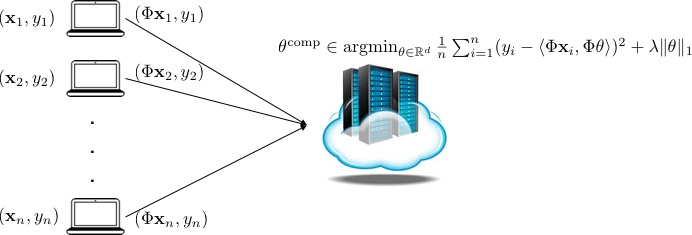
\includegraphics[width=12.5cm]{Picture1.jpg}
%\caption{A vector bundle over a neighborhood of the data, used to produce the output manifold.}
%\end{figure}
\begin{figure}

\begin{picture}(320,160)
 \put(80,00){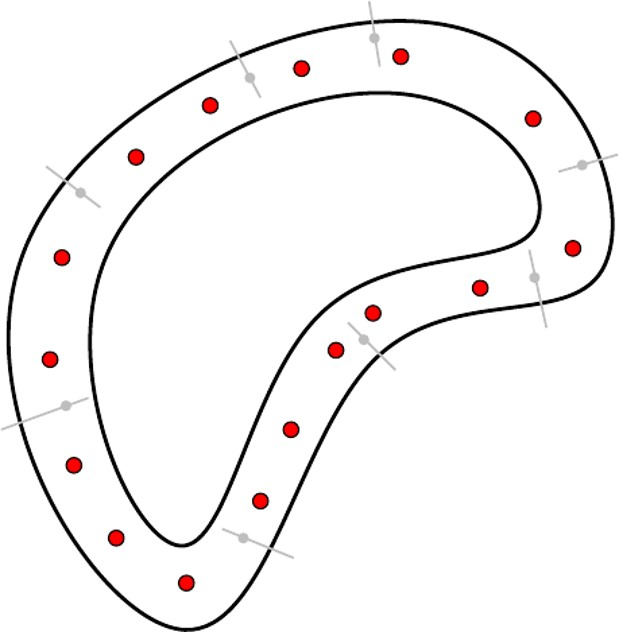
\includegraphics[width=6.0cm]{Picture4.jpg}}

 \put(175,157){$x$}

  \put(185,175){$\hbox{$x$ + Range}(\Pi_x)$}

\end{picture}

\caption{A vector bundle over a neighborhood of the data, used to produce the output manifold.  In the figure,  $x$ is the gray point and $\hbox{$x$ + Range}(\Pi_x)$ is the gray line segment containing $x$.}
\end{figure}

For $x \in \cup_i U_i$, we define $\Pi_x = \Pi_{hi}(A_x)$ where $A_x = \sum_i \a_i(x) \Pi^i$. Let $\tilde{U}_i$ be defined as the $\frac{cr}{d}-$Eucidean neighborhood of $D_i$ intersected with $U_i$. Note that $\Pi_x$ is $\C^2$ when restricted to $\cup_i \tilde U_i$, because the $\a_i(x)$ are $C^2$ and when $x$ is in this set, $c < \sum_i \tilde\alpha_i(x) < c^{-1}$, and for any $i,j$ such that $\a_i(x) \neq 0 \neq \a_j(x)$, we have $\|\Pi^i - \Pi^j\|_F < Cd\de$.
\begin{definition}
The output manifold $\MM_o$ is the set of all points $x \in \cup_i \tilde{U}_i$  such that $\Pi_x F(x) = 0$.
\end{definition}



%The above lemma can be modified in various ways to deliver better bounds. For example, one could combine curved %"patches" instead of discs. At least in the noiseless case this could help.

As stated above,  $\MM_o$ is the set of points $x \in \cup_i \tilde{U_i}$ such that 
\beq \Pi_{hi}(\sum_i \a_i(x)\Pi^i)(\sum_i \a_i(x)\Pi^i(x - p_i)) = 0. \eeq

Using diagonalization and Cauchy's integral formula, we have

\beq\lab{MMo} \frac{1}{2\pi i} \left[\oint_\gamma (zI - (\sum_i \a_i(x)\Pi^i))^{-1}dz\right] \left(\sum_i \a_i(x)\Pi^i(x - p_i)\right) = 0\eeq
where $\gamma$ is the circle of  radius $1/2$ centered at $ 1$.

Let $\sum \a_i(x) \Pi^i = M(x)$, and as stated earlier, $\Pi^i(x - p_i) = F_i(x)$. Let $\Pi_{hi}(M(x))$ be denoted $\Pi_x$.

Then the left hand side of (\ref{MMo}) can be written as 
\beq \oint_\gamma \frac{dz}{2\pi i}\left(\sum_i \a_i(x) (zI - M(x))^{-1}F_i(x)\right). \eeq
for any $v \in \R^{\hat n}$ and and $f:\R^{\hat n} \ra \R^{\tilde n}$ where $\hat n, \tilde n \in \N_+$ let $$\partial_v f(x) := \lim_{\a \ra 0} \frac{f(x + \a v) - f(x)}{\a}.$$

\beq \partial_v  \oint_\gamma \frac{dz}{2\pi i}\left(\sum_i \a_i(x) (zI - M(x))^{-1}F_i(x)\right) & = & \sum_i \a_i(x) \Pi_x (\partial_v F_i(x)) \lab{eq:31}\\
& + &  \sum_i \a_i(x) (\partial_v \Pi_x)  F_i(x) \lab{eq:32}\\
& + &   \sum_i (\partial_v \a_i(x)) \Pi_x  F_i(x). \lab{eq:33}\eeq

%This calculation is continued in the appendix in section~\ref{sec:calc}.

 Let $\|v\| = 1$. Let $\MM_\Pi^d$ denote the set of all projection matrices of rank $d$. This is an analytic submanifold of the space of $n\times n$ matrices.

\begin{claim}\lab{cl:grassmann} The reach of $\MM_\Pi^d$ is greater or equal to $1/2.$
\end{claim}
\begin{proof} This proof appears in Section~\ref{sec:grassmann} of the appendix.
\begin{comment}
Let $$\MM_\Pi := \cup_{\hat d=0}^n \MM_\Pi^{\hat d}.$$ The various connected components 
of $\MM_\Pi$ are the different $\MM_\Pi^d$ (whose dimensions are respectively $(n-d)d$), and by evaluating Frobenius norms, we see that the distance between any two points on distinct connected components is at least $1$. Since it suffices to show that a normal disc bundle of radius less than $1/2$ injectively embeds into the ambient space (which is $\R^{n(n-1)/2}$,)  it suffices to show that
$$reach(\MM_\Pi) = 1/2.$$ Let $x \in \MM_\Pi^d$. Let $z$ belong to the normal fiber at $x$ and let $\|x-z\|_F < 1/2$. Without loss of generality we may (after diagonalization if necessary) take $x = diag(1, \dots, 1, 0, \dots, 0)$ where the number of $1s$ is $d$ and the number of $0s$ is $n-d$. Further, (using block diagonalization if necessary), we may assume that $z$ is a diagonal matrix as well. All the eigenvalues of $z$ lie in $(1/2, 3/2)$ and further the span of the corresponding eigenvectors is the space of eigenvectors of $x$ corresponding to the eigenvalue $1$. Therefore $\Pi_{hi}(z)$ is well defined through Cauchy's integral formula and equals $x$. Thus the normal discs of radius $< 1/2$ do not intersect, and so $reach(\MM_\Pi^d) \geq 1/2.$ Conversely, $\MM_\Pi^0$ is the origin and $\MM_\Pi^1$ contains the point $diag(1, 0, \dots, 0)$. We see that $diag(1/2, 0, \dots, 0)$ is equidistant from $\MM_\Pi^0$ and $\MM_\Pi^1$ and the distance is $1/2$. Therefore $reach(\MM_\Pi^d) \leq 1/2.$ Therefore, 
$$reach(\MM_\Pi^d) \geq reach(\MM_\Pi) = 1/2.$$
\end{comment}
\end{proof}
We first look at the right hand side of (\ref{eq:31}). This can be rewritten as
	\beq \sum_i \a_i(x)\Pi_x \Pi_i v = \Pi_x v + \Pi_x\left( {M(x)} - \Pi_x\right)v.\eeq
%Note that \beq \| {M(x)} - \Pi_x\|_F & \leq & \| {M(x)} - \Pi_j\|_F\\
   %                                                                         & \leq & \sup_i \|\Pi_i - \Pi_j\|_F.\eeq
%Therefore \beq \sup_j \|\Pi_x - \Pi_j\|_F & \leq &  \| {M(x)} - \Pi_x\|_F + \sup_j   \| {M(x)} - \Pi_j\|_F\\
   %                                                             & \leq & 2 \sup_i \|\Pi_i - \Pi_j\|_F.\eeq
                                                                
\beq  \| {M(x)} - \Pi_x\|_F & = & dist(M(x), Tan(\Pi_x, \MM_\Pi^d))\\
& \leq & \sup_i dist(\Pi_i, Tan(\Pi_x, \MM_\Pi^d))\\
& \leq & \sup_i \|\Pi_i - \Pi_x\|_F^2/(2 \, reach(\MM_\Pi^d))\\
& \leq & 4 \sup_{i,j} \|\Pi_i - \Pi_j\|_F^2\\
& \leq & 8d\de^2.\eeq

                                                                          

We look at (\ref{eq:32}) next. Observe that
\beq\nonumber  \left \| \oint_\gamma \frac{dz}{2\pi i} \left(\sum_i \a_i(x) \left(\partial_v ((zI - M(x))^{-1})\right) F_i(x)\right)\right\| & \leq &  \left\| \partial_v \Pi_x \right\|\left\|\sum_i \a_i(x)  F_i(x)\right\|.\eeq
In what follows, we will make repeated use of H\"older's inequality: Let $p, q \in \R$ and $\frac{1}{p} + \frac{1}{q} = 1$, then,
$$\forall x, y \in \R^n, \langle x, y \rangle \leq \|x\|_p \|y\|_q.$$ 

Secondly, we will use the fact that for any ball $U_i$, the number of $j$ such that $U_i \cap U_j$ is nonempty is bounded above by $(Cd)^d$ because of the lower bound of $\frac{cr}{d}$ on the spacing between the $p_i$ and $p_j$ for any two distinct $i$ and $j$. A consequence of this is that any vector $v \in \R^{\bar{N}}$ that is supported on the set of all $j$ such that $U_i \cap U_j \neq \emptyset$ will satisfy \beq \|v\|_{d+2} \leq Cd \|v\|_\infty,\eeq and
\beq \|v\|_{\frac{d+2}{2}} \leq Cd^2 \|v\|_\infty.\eeq

Thirdly, we will use the following bounds on the derivatives of the bump functions at points $x$ that are within a distance of $cr/d$ of $\MM$.
Recall that $\sum_i \ta_i(x)$ is denoted $\ta(x)$. Then we know that $c < \ta(x) < C$ if the distance of $x$ from $\MM$ is less than $cr/d$.
\begin{lemma} \lab{lem:ta2}We have for any $v \in \R^D$ such that $|v| = 1$, and any $x \in \R^D$ such that $dist(x, \MM) \leq \frac{cr}{d}$, \beq   \|(\partial_v \a_i(x))_{i \in[\bar N]}\|_{\frac{d+2}{d+1}} \leq Cd^2. \eeq \end{lemma}
\begin{proof}
This proof appears in section~\ref{sec:ta} in the Appendix.
\begin{comment}
\beq   \|(\partial_v \a_i(x))_{i \in[\bar N]}\|_{\frac{d+2}{d+1}} & \leq &
 \frac{ \|(\partial_v \ta_i(x))_i\|_{\frac{d+2}{d+1}}}{\ta} +   \frac{\|( (\partial_v \ta(x)) \ta_i(x))_i\|_{\frac{d+2}{d+1}}}{\ta^2}\\
& \leq & (c^{-1}) \|Cd(\ta_i(x))_i\|^{\frac{d+1}{d+2}}_1 + (c^{-2}) \| \ta_i(x))_i\|_{\frac{d+2}{d+1}} |\partial_v \ta|\\
& \leq & Cd + C|\partial_v \ta|\\
& \leq & Cd + C\|(\partial_v \a_i)_i\|_{\frac{d+2}{d+1}}\|(1)_i\|_{d+2}\\
& \leq & C d^2 .\eeq
\end{comment}

\end{proof}
\begin{lemma}\lab{lem:ta} We have for any $v \in \R^D$ such that $|v| = 1$, and any $x \in \R^D$ such that $dist(x, \MM) \leq \frac{cr}{d}$, \beq   \|(\partial^2_v \a_i(x))_{i \in[\bar N]}\|_{\frac{d+2}{d}} \leq Cd^4. \eeq \end{lemma}
\begin{proof}This proof appears in section~\ref{sec:ta} in the Appendix.
\begin{comment}
\beq   \|(\partial^2_v \a_i(x))_{i \in[\bar N]}\|_{\frac{d+2}{d}} & = &  \|(\partial^2_v \frac{\ta_i(x)}{\ta(x)})_{i \in[\bar N]}\|_{\frac{d+2}{d}}\\
& = &  \|( \frac{\partial^2_v \ta_i(x)}{\ta(x)} + \frac{(-2)(\partial_v \ta_i(x))(\partial_v\ta(x))}{\ta(x)^2} +  \frac{\ta_i(x)}{\ta(x)^3}(2(\partial_v \ta)^2 - \partial_v^2 \ta(x) (\ta(x)) )_{i \in[\bar N]}\|_{\frac{d+2}{d}}\nonumber. \eeq

We use the triangle inequality on the above expression, and reduce the task of obtaining an upper bound to that of separately obtaining the following bounds.
\begin{claim} We have \beq \|( \frac{\partial^2_v \ta_i(x)}{\ta(x)})_{i \in[\bar N]}\|_{\frac{d+2}{d}} \leq Cd^2, \eeq \end{claim}
\begin{proof} This follows from $c < \ta < C$.\end{proof}
\begin{claim} We have \beq \|(  \frac{(-2)(\partial_v \ta_i(x))(\partial_v \ta(x))}{\ta(x)^2}  )_{i \in[\bar N]}\|_{\frac{d+2}{d}} \leq Cd^3, \eeq \end{claim}
\begin{proof}
We have seen that  $|\partial_v \ta(x)| < Cd^2$. Therefore, 
\beq  \|(  \frac{(-2)(\partial_v \ta_i(x))(\partial_v \ta(x))}{\ta(x)^2}  )_{i \in[\bar N]}\|_{\frac{d+2}{d}} & < & Cd^2 \|(  (\partial_v \ta_i(x))  )_{i \in[\bar N]}\|_{\frac{d+2}{d}}\\
& \leq  & Cd^2 \|(  (\partial_v \ta_i(x))  )_{i \in[\bar N]}\|_{\frac{d+2}{d+1}}\\
& \leq & Cd^3. \eeq
\end{proof}

\begin{claim} \beq \|(   \frac{\ta_i(x)}{\ta(x)^3}(2(\partial_v \ta)^2 - \partial_v^2 \ta(x) (\ta(x)) )_{i \in[\bar N]}\|_{\frac{d+2}{d}} \leq Cd^4. \eeq
\end{claim}
\begin{proof}
The only term that we have not already bounded is $|\partial_v^2 \ta(x)|$. To bound this, we observe that
\beq  C|\partial^2_v \ta| & \leq & C\|(\partial^2_v \ta_i)_i\|_{\frac{d+2}{d}}\|(1)_i\|_{(d+2)/2}\\
& \leq & C d^4 .\eeq Therefore, the entire expression gets bounded by $Cd^4$ as well.
\end{proof}
\end{comment}
\end{proof}



Recall that $ F(x) = \sum\a_i(x) F_i(x).$
\subsection{A bound on the first derivative of $\Pi_xF(x)$}
 We proceed to obtain an upper bound on $ \|\partial_v \Pi_x \|$.

 \beq \|\partial_v \Pi_x \| & \leq & \left(radius(\gamma)\right) \left\|\partial_v ((zI - M(x))^{-1})\right\|\lab{eq:41}\\
 & = & \left(\frac{1}{2}\right) \|(zI - M(x))^{-1}\partial_v M(x) (z I - M)^{-1}\|\\
                                                            & \leq & \left(\frac{1}{2}\right) \|(zI - M(x))\|^{-2}\|\partial_v M(x)\|\\
                                                             & \leq & 8 \|\partial_v M(x)\|\\
                                                             & = & 8 \|\sum_i \partial_v \a_i(x) (\Pi^i-\Pi^1) + \partial_v \sum_i \a_i(x) \Pi_1\|\\
                                                              & \leq & 8 \sum_i |\partial_v \a_i(x)| \de + 0\\
                                                                & \leq &    8   \|(\partial_v \a_i(x))_{i \in[\bar N]}\|_{\frac{d+2}{d+1}}\|(\de)_{i\in[\bar N]}\|_{{d+2}}\\
                                                                  & \leq & C d^3\de . \lab{eq:48}\eeq
 where $C$ is an absolute constant.

Therefore, 
\beq \left \| \oint_\gamma \frac{dz}{2\pi i} \left(\sum_i \a_i(x) \left(\partial_v ((zI - M(x))^{-1})\right) F_i(x)\right)\right\| \leq  Cd^3 \de.\eeq
 Finally, we  bound  (\ref{eq:33}) from above. 
\beq\nonumber  \left\| \oint_\gamma \frac{dz}{2\pi i} \left(\sum_i  \left(\partial_v \a_i(x)\right)  (zI - M(x))^{-1} F_i(x)\right)\right\| & \leq & \left\|\Pi_x \left(\sum_i (\partial_v \a_i(x)) (F_i(x) - F_1(x))\right) \right\| \\ &  + & \left\| \left(\sum_i \partial_v \a_i(x)\right)F_1(x)\right\|\\
& \leq &  \|\Pi_x\| \sum_i |\partial_v \a_i(x)| \| F_i(x) -F_1(x)\| + 0\\
\nonumber & \leq &    \|(\partial_v \a_i(x))_{i\in[\bar N]}\|_{\frac{d+2}{d+1}}\|(F_i(x) -F_1(x))_{i\in[\bar N]}\|_{{d+2}}\\
& \leq & Cd^3 \de.
\eeq 

Therefore \beq \left\| \partial_v \left(  \Pi_x F(x) \right) -  \Pi_x v\right\| \leq C d^3 \de.\eeq
Note also by (\ref{eq:41})-(\ref{eq:48}) that \beq\|\partial_v \Pi_x\| \leq Cd^3\de .\eeq


\subsection{ A bound on the second derivative of $\Pi_x F(x)$}

We now proceed to obtain an upper bound on $\|\partial_v^2 \left(\Pi_x F(x)\right)\|.$

\beq \|\partial_v^2 \left(\Pi_x F(x)\right)\| & \leq & \| (\partial_v^2 \Pi_x) F(x)\|\lab{eq:57}\\
& + & \|2 (\partial_v \Pi_x) \partial_v F(x)\|\lab{eq:58} \\ 
&+ & \|\Pi_x \partial_v^2 F(x)\|.\lab{eq:59}\eeq 

We first bound from above the right side of (\ref{eq:57}).
\beq  (\partial_v^2 \Pi_x)  & = & \partial_v^2\left[\frac{1}{2\pi i}\oint[zI - M(x)]^{-1}dz\right]\\
                                                       & = & \partial_v\left[\frac{1}{2\pi i} \oint(zI - M(x))^{-1}\partial_v M(x) (zI - M(x))^{-1}dz\right]\\
                                                       \nonumber & = & \frac{1}{2\pi i} \oint 2 (zI - M(x))^{-1}\partial_v M(x) (zI - M(x))^{-1} \partial_v M(x) (zI - M(x))^{-1}dz\\ 
& + &  \oint(zI - M(x))^{-1}\partial^2_v M(x) (zI - M(x))^{-1}dz.\eeq
Therefore, \beq  \nonumber \| (\partial_v^2 \Pi_x) F(x)\| & \leq & \sup_{z \in \gamma} \left(C \|(zI - M(x)\|^{-3}\|(\partial_v M(x))^2\| + C \|(zI - M(x)\|^{-2}\|(\partial^2_v M(x))\|\right)\\
                                                         & \leq & C(\|\partial_v M(x) \|^2 + \|\partial_v^2 M(x)\|)\\
                                                        & \leq & Cd^6\de^2 +  \|\partial_v^2 M(x)\| \\
                                                        & = & Cd^6\de^2 + \|\partial_v^2 \sum_i \a_i(x) \Pi_i\|\\
                                                        & \leq & Cd^6\de^2 + \sum_i |\partial_v^2 \a_i(x)(\Pi_i - \Pi_1)|\\
                                                         & \leq & Cd^6\de^2 +  \|(\partial^2_v \a_i(x))_i\|_{\frac{d+2}{d}}\|(\de)_i\|_{\frac{d+2}{2}}\\
                                                          & \leq & Cd^6\de^2 + Cd^6\de.\eeq

Next, we bound  (\ref{eq:58}) from above.
Note that \beq \|\partial_v F(x)\| & \leq & \|(\sum_i \partial_v \a_i(x))(F_i(x) - F_1(x))+\Pi_xv\|\\
& \leq & 1 + C d^3\de.\eeq
\beq \|(\partial_v \Pi_x) \partial_v F(x)\| & \leq &  \|(\partial_v \Pi_x)\| \|\partial_v F(x)\|\\
                                                                  & \leq &   (C d^3 \de ) (1 + d^3 \de)\\
                                                                    & = & C d^3\de + C d^6 \de^2.\eeq

Finally, we bound (\ref{eq:59}) from above.
\beq  \|\Pi_x \partial_v^2 F(x)\| & \leq &  \|\partial_v^2 F(x)\|\\
& \leq & \|\partial_v^2 (F(x) - F_1(x))\|\\
                                                      & \leq & \sum_i |\partial_v^2 \a_i(x)|\| F_i(x) - F_1(x)\|\lab{eq:75}\\
                                                        & + & \sum_i 2| \partial_v \a_i(x)| \|\partial_v F_i(x)- \partial_v F_1(x)\lab{eq:76}\|\\
                                                        & + & \sum_i |\a_i(x)| \|\partial_v^2 F_i(x)\|.\lab{eq:77}
\eeq

We first bound (\ref{eq:75}) from above.
\beq \nonumber  \sum_i |\partial_v^2 \a_i(x)|\| F_i(x)- F_1(x)\| & \leq & \| (|\partial_v^2 \a_i(x)|)_{i\in[\bar N]}\|_{\frac{d+2}{d}}\|(\| F_i(x)- F_1(x)\|)_{i \in [\bar N]}\|_{\frac{d+2}{2}}\\
                                                                        & \leq & (Cd^4)(d^2 \de)\\
                                                                          & = & Cd^6 \de.   
\eeq

Next we bound (\ref{eq:76}) from above.
\beq \nonumber
\sum_i | \partial_v \a_i(x)| \|\partial_v F_i(x) - \partial_v F_1(x)\| & \leq & \|(|\partial_v \a_i(x)|)_{i\in [\bar N]}\|_{\frac{d+2}{d}} \|(\|\partial_v F_i(x)- \partial_v F_1(x)\|)_{i\in[\bar N]}\|_{\frac{d+2}{2}}\\
                                                                             & \leq & C d^4 (d^2\de)\\
                                                                                & = & C d^6\de. \eeq

The term (\ref{eq:77}) is $0$.
  
Therefore \beq\lab{eq:207} \left\| \partial^2_v \left(  \Pi_x F(x) \right) \right\| \leq C d^6 \de.\eeq


Recall that $\MM_o$ is the set of points $x \in \cup_i  \tilde{U}_i$ such that 
\beq \Pi_{hi}(\sum_i \a_i(x)\Pi^i)(\sum_i \a_i(x)\Pi^i(x - p_i)) = 0. \eeq
In particular, $x \in \MM_o \cap U_i$ if and only if $ h(z) = \Pi_i \Pi_{hi}(\sum_i \a_i(z)\Pi^i)(\sum_i \a_i(z)\Pi^i(z - p_i)) = 0,$ where $\Pi^i$ is the orthogonal projection onto the subspace orthogonal to $D_i$, containing the center of $D_i$. We take $U_i$ to be the unit ball and the center of $U_i$ to be the origin and take the linear span of $D_i$ to be $\R^d$.  We split $z$ into its $x$ component (projection onto $\R^d$) and $y$ component (projection orthogonal to $\R^d$). and define $g(x, y) = (x, h(x, y))$. This function is then substituted into the quantitative inverse function theorem of section~\ref{sec:quant} in the appendix.
\section{Hausdorff distance of $\MM_o$ to $\MM$ and the reach of $\MM_o$.}

\begin{theorem}%Suppose $$ \sigma (\sqrt{D} + \ln (N_0)) < \de/d = \frac{Cr^2}{\tau} < \frac{\tau}{Cd^C}.$$ 
With probability at least $1 - N_0^{-C}$, the following is true.
The Hausdorff distance between $\MM_o$ and $ \MM$ is less than $Cd^3 \sqrt{r\de} < \frac{C\tau}{d^C}$ and the reach of $\MM_o$ is at least $\frac{\tau}{Cd^{7}}$.
\end{theorem}
\begin{proof}
Since $ \sigma (\sqrt{D} + \sqrt{\ln (N_0^C)})$ is less than $Cr^2/\tau < \frac{\tau}{Cd^C}$, by Gaussian concentration, with probability at least $ 1 - N_0^{-C}$, every point $y_i = x_i + \zeta_i$ satisfies 
$$|y_i - x_i| = |\zeta_i| <  \sigma (\sqrt{D} + \sqrt{\ln (N_0^C)}) < Cr^2/\tau.$$ All the statements for the rest of this proof will hold with probability at least $1-N_0^{-C}$. Since $X_0$ has a Hausdorff distance $\frac{Cr^2}{\tau}$ to $\MM$, and $X_1$ has a Hausdorff distance $\frac{cr}{d}$ to $\MM$, as a consequence,   the Hausdorff distance between $\cup_i D_i$ and $\MM$ is less than $\de = \frac{Cdr^2}{\tau}$ by subsection~\ref{subsec:algorithm-finddisc}.
The Hausdorff distance between $\cup_i D_i$ and $\MM_o$ is less than \beq Cd^6\de = Cd^{7} \frac{r^2}{\tau} < \frac{C\tau}{d^C}\eeq by the quantitative implicit function theorem (appendix, section~\ref{sec:quant}), applying Taylor's theorem together with (\ref{eq:119a}) and (\ref{eq:122}). Thus, by the triangle inequality, 
the Hausdorff distance between $\MM_o$ and $\MM$ is less than $Cd^{7}{\frac{r^2}{\tau}} < \frac{C\tau}{d^C}.$
Next, we address the reach of $\MM_o$.
By Federer's criterion (Proposition~\ref{thm:federer}) we know that 
\beq reach(\MM_o) = \inf\left\{|b-a|^{2}(2 dist(b, Tan(a)))^{-1}\big| \, a, b \in \MM_o, a \neq b\right\}.\eeq
We wish to prove that $reach(\MM_o) > \frac{\tau}{Cd^7}.$ Let $ a, b \in \MM_o, a \neq b$.

 If $|a - b| > \frac{\tau}{Cd^7}$, then $|b-a|^{2}(2 dist(b, Tan(a)))^{-1} > \frac{\tau}{Cd^7},$ because 
\beqs |b-a| \geq dist(b, Tan(a)). \eeqs

Therefore, we may suppose that $|a-b| \leq \frac{\tau}{Cd^7}$.
By the bound on the Hausdorff distance between $\MM$ and $\MM_o$, the respective distances of $a$ and $b$ to the images of their projections onto $\MM$, which we denote $a'$ and $b'$ respectively, are less than $Cd^3 \sqrt{r \de}$. By the quantitative implicit function theorem (appendix, section~\ref{sec:quant}) and the covering property of $\{U_i\}$, $\MM_o$ is a $C^2-$submanifold of $\R^n$. Therefore $Tan(a)$ is a $d-$dimensional affine subspace. By  (\ref{eq:119a}) and (\ref{eq:122}) the Hausdorff distance between the two unit discs $Tan(a) \cap B(a, 1)$ and $(Tan_\MM(a') \cap B(a',  1)) + (a - a')$ which are centered at $a$, is bounded above by \beq \lab{eq:C1dist} Cd^3 \sqrt{\de/r} = Cd^{7/2} \sqrt{r/\tau} = \frac{1}{Cd^{C}}.\eeq Then, $\MM$ and $\MM_o$ are $Cd^3 \sqrt{r \de}$ close in Hausdorff distance and 
$(\MM_o \cap B(a, 2|a-b|))$ and $(\MM \cap B(a',  2|a-b|))$ are $Cd^3 \sqrt{\de/r}|a-b| = \frac{1}{Cd^{C}}$ close in $C^1$ over the maximal subset $U^a$ of $Tan(a)$ on which both are defined as graphs of functions  (respectively $\hat{f}_o$ and $\hat{f}$) whose range is $Nor(a)$, the fiber of the normal bundle at $a$ by Lemma~\ref{lem:6}; please see section~\ref{sec:GeomPrelim} in the appendix. This subset contains $(Tan(a) \cap B(a, 3|a-b|/2))$ because we further know by (\ref{eq:C1dist}) and the reach of $\MM$ being at least $\tau$,
that the  $C^1$ norm of $\hat{f}$ on $(Tan(a) \cap B(a, 3|a-b|/2))$ is at most $(Cd^7)^{-1}$. 
Therefore, the  $C^1$ norm of $\hat{f}_o$ on $(Tan(a) \cap B(a, 3|a-b|/2))$ is at most $(Cd^7)^{-1}$. 
But using this and the Hessian bound of $C d^6 \de$ from (\ref{eq:207}), we also know that the Hessian of $\hat{f}_o$ is bounded above by $C d^7/\tau$. But now, by Taylor's theorem,  $dist(b, Tan(a)) \leq \sup \|Hess \hat{f}_o\||a-b|^2/2,$ where the supremum is taken over $(Tan(a) \cap B(a, 3/2|a-b|))$. This, we know is bounded above by $Cd^7|a-b|^2/\tau$. Substituting this into Federer's criterion for the reach, we see that $$reach(\MM_o) \geq \frac{\tau}{Cd^7}.$$
 %Since $r = \frac{\tau}{Cd^C}$. This means that $\de < \frac{C\tau}{d^C}$.
\end{proof}

\begin{comment}
This is where the content of your paper goes.  Remember to:
\begin{itemize}
\item Limit the main text (without references and appendices) to 12 PMLR-formatted pages (i.e., using this template).
\item Include, either in the main text or the appendices, all details, proofs
  and derivations required to substantiate the results.
\item Include {\em in the main text} enough details, including proof
  details, to convince the reviewers of the contribution, novelty and significance of the submissions.
\item Not include author names (this is done automatically), and to
  the extent possible, avoid directly identifying the authors.  You
  should still include all relevant references, including your own,
  and any other relevant discussion, even if this might allow a
  reviewer to infer the author identities.
  \end{itemize}
\end{comment}


% Acknowledgments---Will not appear in anonymized version
\acks{Ch.F. was partly supported AFOSR, grant DMS-1265524, and NSF, grant FA9550-
12-1-0425. S.I. was partly supported RFBR, grant 14-01-00062, Y.K. was partly
supported by EPSRC and the AXA professorship, M.L. was supported by Academy
of Finland, grants 273979 and 284715, and H.N. was partly supported by NSF
grant DMS-1620102 and a Ramanujan Fellowship.}


\bibliography{kpca_colt_fitting}


\appendix

\section{Geometric Preliminaries}\lab{sec:GeomPrelim}

Let $\MM \in \G(d, V, \tau)$. In the remainder of this section, for $x \in \MM$ denote  the orthogonal projection from $\R^n$
 to the affine subspace tangent to $\MM$ at $x$,  $Tan(x)$ by $\Pi_{x}$. 


\begin{lemma}\lab{lem:3}
For each $p \in \MM,$ such that $Tan(p) = \{(z_1, z_2) \in \R^d\oplus \R^{n-d}| A z_1 + b= z_2\}$ for some matrix $A(p)$ and vector $b(p)$, there  exists a neighborhood $ V \subseteq \R^n$ of $p$, an open set $U \in \R^d$ and a $\C^2$ function $F: U \ra \R^{n-d}$ with $DF(u)$ of rank $d$ for all $u \in U$ such that 
\beq\lab{eq:ast2} \MM \cap V = ((u, F(u)), u \in U \cap \R^d). \eeq
\end{lemma}
\begin{proof}
Let $U, W, \phi, \psi$ be as in the definition of a $C^2$ manifold. Since $\phi \circ \psi = id$, $D\psi$ has rank $d$ at each point of $W$, in particular $q = \phi(p)$. Therefore, 
\beq\lab{eq:ast1} \det\left(\frac{\partial}{\partial w_1}\Pi_{\R^d} \circ \psi, \dots, \frac{\partial}{\partial w_d}\Pi_{\R^d} \circ \psi\right) \neq 0\eeq holds at $q$.
By (\ref{eq:ast1}), we can apply the inverse function theorem to $\Pi_{\R^d} \circ \psi$ at $u_0= \Pi_{\R^d}\circ\psi(q)$ to see that $f = (\Pi_d \circ \psi)^{-1}:U' \ra \R^d$ exists, is $\C^2$ and $Df$ has rank $d$ at each $u \in U'$ for some neighborhood $U'$ (possibly smaller than $U$) of $\Pi_{\R^d}q.$  Setting $F = \Pi_{\R^{n-d}}\circ \psi\circ f$, we obtain (\ref{eq:ast2}).
\end{proof}
\begin{lemma} \lab{cl:g1sept}
Suppose that $\MM \in \G(d, V, \tau)$. Let \beqs U:= \{y\big||y-\Pi_xy| \leq \tau/4\} \cap  \{y\big||x-\Pi_xy| \leq \tau/4\}.\eeqs 
Then, $$\Pi_x(U \cap \MM) = \Pi_x(U).$$
\end{lemma}
\begin{proof}
Without loss of generality, we will assume $\tau/2 = 1$, and $x = \{0\}$, and $Tan(x) = \R^d$.
Let $\NN = U \cap \MM$. We will first show that $\Pi_0(\NN) = B_d$, where $B_d$ is the unit ball in $\R^d.$ Suppose otherwise, then let $\emptyset \neq Y := B_d \setminus \Pi_0(\NN)$. Note that $\NN$ is closed and bounded and is therefore compact. The image of a compact set under a continuous map is compact, therefore $\Pi_0(\NN)$ is compact. Therefore $\R^d \setminus \Pi_0(\NN)$ is open. Let $x_1$ be a point of minimal distance from $0 = \Pi_0(0) \subseteq \Pi_0(\NN)$ among all points in the closure $Z$ of $\R^d \setminus \Pi_0(\NN)$. Since $\emptyset \neq Y$ and  $\R^d \setminus \Pi_0(\NN)$ is open, $|x_1| < 1$. Since $Tan(0)= \RR^d$ and $\MM$ is a closed  imbedded $C^2-$submanifold, $0$ does not belong to $Z$. Therefore $x_1 \neq 0$. By Federer's criterion for the reach, $\forall y_1 \in \Pi_0^{-1}(x_1) \cap \NN$, \beq dist(y_1, Tan(0)) \leq \frac{\|y_1\|^2}{4}.\eeq
Therefore, $\forall y_1 \in \Pi_0^{-1}(x_1) \cap \NN$, \beq dist(y_1, \R^d) \leq \frac{dist(y_1, \R^d)^2 + |x_1|^2}{4} .\eeq
Noting that $2 \geq 1 \geq dist(y_1, \R^d)$ and solving the above quadratic inequality, we see that \beq |y_1 - x_1|/2 & \leq & 1 - \sqrt{ 1 - \left(\frac{|x_1|}{2}\right)^2}\\ & \leq &  \left(\frac{|x_1|}{2}\right)^2.\eeq

This implies that \beq\lab{eq:54} |y_1 - x_1| \leq \frac{1}{8} < \frac{\tau}{8}. \eeq
Again by Federer's criterion, for any $z \in \Pi_0^{-1} (|x_1| B_d) \cap \NN$, 
\beq |z -\Pi_{y_1}(z)|/2 & \leq & 1 - \sqrt{1 - \left(\frac{|y_1 - \Pi_{y_1} z|}{2}\right)^2}\\ & \leq & \left(\frac{|y_1 - \Pi_{y_1} z|}{2}\right)^2. \eeq

 By Lemma~\ref{lem:3} and (\ref{eq:54}), we have the following.

\begin{claim}\lab{cl:1} Let $y_1 \in \Pi_0^{-1}(x_1) \cap \NN$. Then there exists $v \in \partial B_d$ such that  if $y_1' \in Tan(y_1)$ then $\langle y_1'-y_1, v\rangle = 0$.
\end{claim}

Let $\ell = \{\la v| \la \in \R\}$ and let $\Pi_\ell$ denote the orthogonal projection on to $\ell$. Then, $$\Pi_\ell(|x_1| B_d) = \{\la v | \la \in [-|x_1|, |x_1|]\}.$$ By Claim~\ref{cl:1}, $\Pi_\ell(Tan(y_1))$ is the single point $\Pi_\ell(y_1)$. Let $\Pi_\ell(y_1) = \la_0 v$. Let $x_2 = |x_1| v$ if $\la_0 \leq 0$ and $x_2 = -|x_1|v$ if $\la_0 > 0$. Let $y_2 \in \Pi_0^{-1}(x_2) \cap \NN$. 
Then,
\beq  |x_1| & \leq & |\Pi_\ell(y_1) - x_2|\\
 & \leq &  dist(y_2, Tan(y_1))\\
                            & \leq &  \frac{|y_2 - y_1|^2}{4}\\
                             & \leq & \frac{2|y_2 - x_2|^2 + |x_1 - x_2|^2 +2 |y_1 - x_1|^2}{4}\\
                            & \leq & \frac{2\left(\frac{|x_2|^2}{2}\right)^2 + 4 |x_1|^2 + 2\left(\frac{|x_1|^2}{2}\right)^2}{4}\eeq



Therefore, $$\a := |x_1| \leq |x_1|^4/4 + |x_1|^2.$$
Therefore, $1 \leq  \a^3/4 + \a$. This implies that \beq |x_1| & > & \frac{1}{2}.\eeq

\end{proof}

\begin{lemma}\lab{lem:6}

Suppose that $\MM \in \G(d, V, \tau)$. Let \beqs \hat U:= \{y\big||y-\Pi_xy| \leq \tau/8\} \cap  \{y\big||x-\Pi_xy| \leq \tau/8\}.\eeqs 
There exists a $C^{2}$ function $F_{x, \hat U}$ from $\Pi_x( \hat U)$ to $\Pi_x^{-1}(\Pi_x(0))$ such that
\beqs  \{ y + F_{x, \hat U}(y) \big | y \in \Pi_x(\hat U)\} = \MM \cap \hat U.\eeqs 
Secondly,
 let $z \in \MM \cap \hat U$ satisfy $|\Pi_x(z) - x| = \de.$ Let $z$ be taken to be the origin and let the span of the first $d$ canonical basis vectors be denoted $\R^d$ and let $\R^d$ be a translate of $Tan(x)$. Let the span of the last $n-d$ canonical basis vectors be denoted $\R^{n-d}$. In this coordinate frame, let a point $z' \in\R^n$ be represented as  $(z'_1, z'_2)$, where $z'_1 \in \R^d$ and $z'_2 \in \R^{n-d}$.
 By the preceding lemma, there exists an $(n-d) \times d$ matrix $A_z$ such that  \beq \lab{eq:36.1} Tan(z) = \{(z'_1, z'_2)| A_z z'_1 - I z'_2 = 0\}\eeq where the identity matrix is $(n-d) \times (n-d)$. For $ \de < \tau/8$, let $z\in \MM \cap \{z\big||z-\Pi_xz| \leq \de\} \cap \{z\big||x-\Pi_xz| \leq \de\}$. Then $\|A_z\|_2 \leq 20 \de/\tau.$
\end{lemma}
\begin{proof}Let
\beqs U:= \{y\big||y-\Pi_xy| \leq \tau/4\} \cap  \{y\big||x-\Pi_xy| \leq \tau/4\}.\eeqs 
We will first show that there exists a function $F_{x, \hat U}$ that satisfies the given conditions and then show that it is $C^{2}$. Let $z \in \MM \cap \hat U$ satisfy $|\Pi_x(z) - x| = \de.$ Let $z$ be taken to be the origin and let the span of the first $d$ canonical basis vectors be denoted $\R^d$ and let $\R^d$ be a translate of $Tan(x)$. Let the span of the last $n-d$ canonical basis vectors be denoted $\R^{n-d}$. In this coordinate frame, let a point $z' \in\R^n$ be represented as  $(z'_1, z'_2)$, where $z'_1 \in \R^d$ and $z'_2 \in \R^{n-d}$. By the preceding lemma, there exists a matrix $A$ such that  \beq \lab{eq:36} Tan(z) = \{(z'_1, z'_2)| Az'_1 - I z'_2 = 0\}.\eeq
Further, a linear algebraic calculation shows that \beq dist(z', Tan(z)) = \bigg\|(I + A A^T)^{-1/2}(Az_1' - I z_2')\bigg\|_2.\eeq Let $S^{d-1}_\de$ denote the $d-1-$dimensional sphere of radius $\de$ centered at the origin contained in $\R^d$. By the preceding lemma, there is a point $\tilde z \in \MM$ for every $z' \in S^{d-1}_\de$ such that $\tilde z \in U$, $\Pi_x \tilde z = \Pi_x z'$ and 
\beq \left\|\tilde z - \Pi_x \tilde z \right\| \leq \frac{\left\|x - \Pi_x \tilde z \right\|^2}{\tau} = \frac{4 \de ^2}{\tau}.\eeq
Therefore, \beq \left\|\tilde z - z'\right\| = \left\| \tilde z - ((\Pi_x \tilde z) -x_2)\right\| \leq  \frac{4 \de ^2}{\tau} +  \frac{ \de ^2}{\tau} =  \frac{5 \de ^2}{\tau}. \eeq
Therefore, 
\beq dist(z', Tan(z)) & \leq & dist(\tilde z, Tan(z)) +  \left\|\tilde z - z'\right\| \\ & \leq & \frac{|z - \tilde z|^2}{\tau} + \frac{5\de^2}{\tau}\\
& = & \frac{|z-z'|^2 + |z' - \tilde z|^2}{\tau} + \frac{5\de^2}{\tau}\\ & \leq & \frac{\de^2 + (8\de^2/\tau)^2}{\tau} + \frac{5\de^2}{\tau}. \eeq
Therefore, for any $z_1' \in S^{d-1}_\de$, 
\beq \left\|(I + A A^T)^{-1/2}(Az_1')\right\|_2 \leq \frac{\de^2}{\tau}\left(6 + \frac{64 \de^2}{\tau^2}\right). \eeq
Thus,
\beq \left\|(I + A A^T)^{-1/2}(A)\right\|_2 \leq  \frac{\de}{\tau}\left(6 + \frac{64 \de^2}{\tau^2}\right) =:  \de'. \eeq
Therefore,  we see that
\beq  \left\|(I + A A^T)^{-1/2}(AA^T) (I + A A^T)^{-1/2}\right\|_2 \leq \de'^2.\eeq
Let $\|A\|_2 = \la$. We then see that $\la^2$ is an eigenvalue of $AA^T$. Therefore, 
\beq \frac{\la^2}{1+\la^2} \leq \de'^2.\eeq
This gives us $\la^2 \leq \frac{\de'^2}{1 - \de'^2 }$, which implies that
\beq\lab{eq:la} \la \leq \frac{\de'}{\sqrt{1 - \de'^2}}. \eeq

We will use this to show that , $\Pi_x^{-1}(\Pi_x z) \cap \MM \cap U$ contains the single point $z$.
Suppose to the contrary, there is a point $\hat z \neq z$ that also belongs to  $ \Pi_x^{-1}(\Pi_x z) \cap \MM \cap U$. Then, \beq dist(\hat z, Tan(z)) \leq \frac{\|\hat z_2\|^2}{\tau},\eeq where $\|\hat z_2\| \leq 2 \de^2/\tau$. Thus, $$\|\hat z_2\| \leq \frac{\|\hat z_2\|^2 \|I+ A A^T\|^{1/2}}{\tau}.$$ Therefore,
\beq 1 \leq \|\hat z_2\|(1/\sqrt{(1 - \de'^2)})/\tau \leq \frac{2 \de^2}{\tau^2\sqrt{1 - \de'^2}}. \eeq


Therefore \beq 1-\de'^2 \leq \frac{2\de^2}{\tau^2},\eeq and so 
\beq \de' \geq 1 - 2\de^2/\tau^2. \eeq
assuming $\de \leq \frac{\tau}{8}$, 
\beq \de' \leq \frac{7\de}{\tau}. \eeq

Therefore $$2 \de^2/\tau^2 + 7\de/\tau \geq 1.$$ This implies that $\de /\tau > 1/8$. This is a contradiction.

By (\ref{eq:36}) and Lemma~\ref{lem:3}, $F_{x, U}$ is $C^2$.
\end{proof}


\section{Quantitative inverse and implicit function theorems}\lab{sec:quant}
We now prove versions of the implicit and inverse function theorems with quantitative bounds on the second derivatives that do not depend on the dimensions involved.

We begin with the inverse function theorem.

Let $g: \R^p \ra \R^p$ be a $\C^2$ function on whose derivatives the following bounds hold.

At any point $x \in B_p(0, 1)$, \beq\lab{eq:11}\|Jac_g - I\| \leq \eps^2/4\eeq for some $\eps \in [0, 1]$

For any non-zero vector $v$ and $x$ as before, \beq\lab{eq:12}\left\|\frac{\partial^2 g(x)}{\partial v^2}\right\| \leq \left(\frac{\eps^2}{4}\right) |v|^2\eeq for the same $\eps$.

By (\ref{eq:11}), for any $x \neq x'$, both belonging to $B_p(0, 1)$, $$|g(x) - g(x') - (x - x')| \leq |x-x'| (1/4),$$ which implies that $g(x) \neq g(x')$. Applying the Inverse Function Theorem (\cite{Narasimhan}), 
there exists a function $f: g(B_p(0, 1)) \ra B_p(0, 1)$ such that 
$f(g(x)) = x$, for all $x \in B(0, 1)$. Let $\tf = w\cdot f$ for some fixed non-zero vector $w$. Let $g = (g_1, \dots, g_p)$, where each $g_i$ is a real-valued function. The Jacobian of the identity function is $I$. Therefore, by the chain rule,
\beq \lab{eq:12.01} \left(\left(\frac{df_i}{dg_j}\right)_{i, j \in [p]}\right) Jac_g = I, \eeq implying by (\ref{eq:11}) that

\beq \lab{eq:12.02} \left\| \left(\left(\frac{df_i}{dg_j}\right)_{i, j \in [p]}\right)\right\| \leq (1 - \eps^2/4)^{-1}\eeq

The second derivative of a linear function is $0$ and so \beq 0 = \frac{\partial^2 \tf (g) }{\partial v^2} (x) =  \sum_{i, j} \frac{d^2\tf}{{dg_i}{dg_j}}\left(\frac{dg_i}{dv}\right)\left(\frac{dg_j}{dv}\right) + \sum_j \frac{d\tf}{dg_j}\left( \frac{d^2g_j}{dv^2}\right). \eeq
Therefore, 

 \beq  \sum_{i, j} \frac{d^2\tf}{{dg_i}{dg_j}}\left(\frac{dg_i}{dv}\right)\left(\frac{dg_j}{dv}\right) = (-1) \sum_j \frac{d\tf}{dg_j}\left( \frac{d^2g_j}{dv^2}\right). \eeq
and so by Cauchy-Schwartz, 

\beq\lab{eq:12.1}  \left|\sum_{i, j} \frac{d^2\tf}{{dg_i}{dg_j}}\left(\frac{dg_i}{dv}\right)\left(\frac{dg_j}{dv}\right) \right| \leq \left \| \left(\left(\frac{d\tf}{dg_j}\right)_{j \in [p]}\right)\right\| \left\| \left(\left( \frac{d^2g_j}{dv^2}\right)_{j \in [p]}\right) \right\|. \eeq

By (\ref{eq:11}) there exists a unit vector $\tilde{v}$ such that 
\beq\lab{eq:12.2} \left|\sum_{i, j} \frac{d^2\tf}{{dg_i}{dg_j}}\left(\frac{dg_i}{d\tilde v}\right)\left(\frac{dg_j}{d \tilde v}\right) \right| =  \left\|Hess\, \hat{F}\right\|  \left\|\frac{dg}{d\tilde v}\right\|^2 \geq  \left\|Hess\, \hat{F}\right\|  \inf \limits_{\|v\| = 1}\left\|\frac{dg}{dv}\right\|^2. \eeq 

Together (\ref{eq:12}), (\ref{eq:12.02}), (\ref{eq:12.1}) and (\ref{eq:12.2}) imply that 

\beq \left\|Hess\, \hat{F}\right\|  \inf \limits_{\|v\| = 1}\left\|\frac{dg}{dv}\right\|^2 \leq \left\|\left(\left(\frac{df_i}{dg_j}\right)_{i, j \in [p]}\right)w\right\| \sup\limits_{\|v\|=1}\left(\frac{\eps^2}{4}\right) \|v\|^2 \leq \left(\frac{\eps^2}{4 - \eps}\right)\|w\|. \eeq
It follows that 
\beq \left\|Hess\, \hat{F}\right\|  \leq \left(\frac{\eps^2}{4 - \eps}\right)\|w\| \sup \limits_{\|v\| = 1}\left\|\frac{dg}{dv}\right\|^{-2} \leq \left(\frac{16\eps^2}{(4-\eps)^3}\right) \|w\|. \eeq

Next, consider the setting of the Implicit Function Theorem. Let $h: \R^{m+n} \ra \R^n$ be a $\C^2-$function,
$$ h:(x, y) \mapsto h(x, y).$$
Let $g:B_{m+n} \ra \R^{m+n}$ be defined by $$g:(x, y) \mapsto (x, h(x, y)).$$

 Suppose the Jacobian of  $g$, $Jac_g$ satisfies $$\left\|Jac_g - I\right\| < \eps^2/4$$ on $B_{m+n}$ and that for any vector $v \in \R^{m+n}$, $$\left\|\frac{\partial^2 g(x)}{\partial v ^2}\right\| \leq \left(\frac{\eps^2}{4}\right)\|v\|^2$$ where $\eps \in [0, 1]$.
Suppose also that $\|g(0)\| < \frac{\eps^2}{20}$ for the same $\eps$.

Let $p = m+n$. Then, applying the inverse function theorem, we see that defining $f$ and $\hat F$ as before, and choosing $\|w\|= 1$, 

\beq\lab{eq:15} \left\|Hess\, \hat{F}\right\|  \leq \frac{16\eps^2}{(4-\eps)^3}. \eeq

\begin{lemma}\lab{lem:4}
On the domain of definition of $f$, \ie $g(B_{m+n})$ 
$$f ((x, y)) = (x, e(x, y))$$ for an appropriate $e$ and in particular, for $\|x\| \leq \frac{\eta}{2}$, where $\eta \in [0, 1]$,
$$f((x, 0)) = (x, e(x, 0))$$ and $$\|(x, e(x, 0))\| \leq \frac{8}{5}\left( \frac{\eps^2}{20} + \frac{\eta}{2}\right).$$
 Finally, for any $w \in \R^n$ such that $\|w\| = 1$, 
\beq \|Hess (e\cdot w)\| \leq \frac{16\eps^2}{(4-\eps)^3}.\eeq
\end{lemma}

\begin{proof}
It suffices to prove that if $z = (x, y) \in \R^p$ and $\|z\| \leq \eta/2$, where $\eta \in [0, 1]$,
then there exists a point $\hz$, where $\|\hz\| \leq \frac{8}{5}\left( \frac{\eps^2}{20} + \frac{\eta}{2}\right), $ such that $g(\hat z) = z.$
We will achieve this by analysing  Newton's method for finding a sequence $\hat z_0, \dots, \hat z_k, \dots $ converging to a point $\hat z $ that satisfies  $g(\hat z) = z$. We will start with $\hat z_0 = 0.$ 

The iterations of Newton's method proceed as follows.

For $i \geq 0$, 
\beq \hz_{i+1} = \hz_i - J_g^{-1}(\hz_i)(g(\hz_i) - z). \eeq
\begin{claim}

We shall first show that for any $i \geq 0$, $\|\hz_i\| \leq \frac{8}{5}\left( \frac{\eps^2}{20} + \frac{\eta}{2}\right).$ 
\end{claim}
\begin{proof}
Observe that \beq\|\hz_{i+1} - \hz_i\| = \|J_g^{-1}(\hz_i)(g(\hz_i) - z) \|.\eeq

For $i=0$, \beq \|g(\hz_i) - z\| \leq \frac{\eps^2}{20} + \frac{\eta}{2}.\eeq and since $\|J_g^{-1}(\hz_i)\| \leq \frac{1}{1-\epsilon/4} \leq 4/3$, therefore 
\beq\lab{eq:19} \|\hz_{i+1} - \hz_i\| \leq \left(\frac{4}{3}\right)\left( \frac{\eps^2}{20} + \frac{\eta}{2}\right) .\eeq

Suppose $i \geq 1$. 
\beq \lab{eq:20} g(\hz_i) - z =   g\left(\hz_{i-1} - J_g^{-1}(\hz_{i-1})(g(\hz_{i-1}) - z)\right) - z. \eeq
Using the integral form of the remainder in Taylor's theorem, the right hand side of (\ref{eq:20}) equals
$$g(\hz_{i-1}) + J_g(\hz_{i-1})\left( - J_g^{-1}(\hz_{i-1})(g(\hz_{i-1}) - z) \right) + \Lambda  - z,$$ which simplifies to $\Lambda$,
where $$\Lambda = \int_0^1 {(1-t)} (\hz_{i} - \hz_{i-1})^T Hess_g(\hz_{i-1} + t(\hz_{i} - \hz_{i-1}))(\hz_{i} - \hz_{i-1})dt.$$
The norm of $\Lambda$ is bounded above as follows. Note that by the induction hypothesis, $\|\hz_i\| \leq \frac{8}{5}\left( \frac{\eps^2}{20} + \frac{\eta}{2}\right),$ and $\|\hz_{i-1}\| \leq \frac{8}{5}\left( \frac{\eps^2}{20} + \frac{\eta}{2}\right)$, which places both $\hz_i$ and $\hz_{i-1}$ within the unit ball. Therefore $\|(\hat z_{i} - \hat z_{i-1})^T Hess_g(\hat z_{i-1} + t(\hat z_{i} - \hat z_{i-1}))(\hat z_{i} - \hat z_{i-1})\| \leq (\eps^2/4)\|\hat z_i - \hat z_{i-1}\|^2$ for any $t \in [0, 1]$.
$$\|\Lambda\| \leq  \int_0^1 {(1-t)} \|(\hz_{i} - \hz_{i-1})\|^2 (\eps^2/4) dt =   \left(\frac{\eps^2}{8}\right) \|(\hz_{i} - \hz_{i-1})\|^2.$$

Therefore  \beq\|\hz_{i+1} - \hz_i\| = \|J_g^{-1}(\hz_i)(g(\hz_i) - z) \| \leq \left(\frac{4}{3}\right)\left(\frac{\eps^2}{8}\right) \|(\hz_{i} - \hz_{i-1})\|^2  = \left(\frac{\eps^2}{6}\right) \|(\hz_{i} - \hz_{i-1})\|^2.\eeq

By recursion,
\beq\lab{eq:22} \|\hz_{i+1} - \hz_i\| \leq \left(\frac{\eps^{2i}}{6^i}\right)\|\hz_1 - \hz_0\|^{2^i}. \eeq
Therefore, \beq  \|\hz_{i+1}\| = \|\hz_{i+1} - \hz_0\| \leq \sum_{j = 1}^i \|\hz_{j+1} - \hz_j\| \leq  \frac{\|\hz_1 - \hz_0\|}{1 - \frac{\eps^2}{6}} \leq \left(\frac{4}{3}\left( \frac{\eps^2}{20} + \frac{\eta}{2}\right)\right)\left(\frac{6}{5}\right) = \frac{8}{5}\left( \frac{\eps^2}{20} + \frac{\eta}{2}\right). \eeq
\end{proof}
 Recall that 
$g:B_{m+n} \ra \R^{m+n}$ is given by $$g:(x, y) \mapsto (x, h(x, y)).$$ Since $g$ is injective, it  follows that on the domain of definition of $f$, \ie $g(B_{m+n})$ 
$$f ((x, y)) = (x, e(x, y))$$ for an appropriate $e$.  
By (\ref{eq:19}) and (\ref{eq:22}) $(\hz_0, \dots, \hz_i, \dots)$ is a Cauchy sequence, and therefore has a unique limit point. By the preceding Claim, this limit $\hz$ satisfies $\|\hz\| \leq \frac{22}{25} < 1$. Therefore any point in $B_m\times B_n$ of the form $(x, 0)$ where $\|x\| = \frac{\eta}{2} \leq \frac{1}{2}$ belongs to $g(B_{m+n})$. Further, 
$$\|f((x, 0))\| \leq \frac{8}{5}\left( \frac{\eps^2}{20} + \frac{\eta}{2}\right).$$ In particular, setting $\eta = 0$, we have \beq \|f((0, 0))\| \leq \frac{2\eps^2}{25}. \lab{eq:119a} \eeq

By (\ref{eq:12.02}) the function $e$ satisfies, for $\|x\| \leq 1/2$, 
\beq \lab{eq:De} \|D_x e\|^2 & = & \|D_x f\|^2 - 1\\
& \leq & (1 - \eps^2/4)^{-2} - 1\\
& \leq & \epsilon^2. \lab{eq:122}\eeq

By (\ref{eq:15}) the function $e$  satisfies, for any $w \in \R^n$ such that $\|w\| = 1$, 
\beq \|Hess (e\cdot w)\| \leq \frac{16\eps^2}{(4-\eps)^3}.\eeq
\end{proof}

\section{Finding good discs}\lab{sec:follows}

Let $G_\sigma^z$ be the spherical gaussian measure whose  variance (of the marginal along any fixed direction) is $\sigma^2$ and center $z$. When $z$ is the origin, we will drop the superscript.
Let $\hat \mu  = \mu * G_\sigma$ be the distribution from which the $y_i$ are drawn. 
We will need the following theorem which follows from Theorem 3.2.3 in  \cite{federer_book}.

\begin{theorem}
Let $\mathcal{L}^m$ denote the $m-$dimensional Lebesgue measure and $\mathcal{H}^m$ denote the $m-$dimensional Hausdorff measure.
Suppose $f:A \ra \R^n$ be a $1 \ra 1$ $C^2$ function with $m \leq n$ where $A$ is a $\mathcal{L}^m-$measurable subset of $\R^m$ and $J_m f$ is the Jacobian of $f$.  If $u$ is a $\mathcal{L}^m$ integrable function, then 
\beq \int_{\R^m} u(x) J_m f(x) \mathcal{L}^m (dx) = \int_{\R^n} u(f^{-1}(y)) \mathcal{H}^m(dy). \eeq
\end{theorem}



\subsection{Learning unit discs that approximate the data locally}
\label{subsec:algorithm-finddisc}

Let $X$ be a finite set of points in $E= \mathbb{R}^D$ and $X \cap B_1(x) := \{x, \tilde{x}_1, \dots, \tilde{x}_s\}$ be a set of points within a Hausdorff distance $\delta$ of some (unknown) unit $d$-dimensional disc $D_1(x)$ centered at $x$.  Here $B_1(x)$ is the set of points in ${\mathbb R}^D$ whose distance from $x$ is less or equal to $1$. We give below a simple algorithm that finds a unit $d$-disc centered at $x$ within a Hausdorff distance $C{d}\delta$ of $X_0:= X \cap B_1(x)$, where $C$ is an absolute constant.

The basic idea is to choose a near orthonormal basis from $X_0$ where $x$ is taken to be the origin and let the span of this basis intersected with $B_1(x)$ be the desired disc.
This algorithm appeared previously in \cite{recons}, but has been included in the interest of readability.

\underline{Algorithm FindDisc:}
\begin{enumerate}
\item Let $x_1$ be a point that minimizes $ |1 - |x- x'||$ over all $x' \in X_0$.
\item Given $x_1, \dots x_m$ for $m \leq d-1$, choose $x_{m+1}$ such that $$\max(|1-|x- x'||, |\langle x_1/|x_1|, x'\rangle|, \dots, |\langle x_m/|x_m|, x'\rangle|)$$ is minimized among all $x' \in X_0$ for $x'= x_{m+1}$.
    \end{enumerate}
Let $\tilde{A}_x$  be the affine $d$-dimensional subspace containing $x, x_1, \dots, x_n$, and the unit $d$-disc $\tilde{D}_1(x)$ be $\tilde{A}_x \cap B_1(x)$. Recall that for two subsets $A, B$ of $\R^D$, $d_H(A, B)$ represents the Hausdorff distance between the sets. The same letter $C$ can be used to denote different constants,
even within one formula.

\begin{lemma}
Suppose there exists a $d$-dimensional affine subspace $A_x$ containing $x$ such that $D_1(x) = A_x \cap B_1(x)$ satisfies $d_H(X_0, D_1(x)) \leq \delta$.
Suppose $0 < \delta < \frac{1}{2d}$. Then $d_H(X_0, \tilde{D}_1(x)) \leq  C{d}\delta$, where $C$ is an absolute constant.
\end{lemma}
\begin{proof}
Without loss of generality, let $x$ be the origin. Let $d(x, y)$ be used to denote $|x-y|$.
We will first show that for all $m \leq d-1$,
$$\max\left(|1-d(x, x_{m+1})|, \left | \left\langle \frac{x_1}{|x_1|}, x_{m+1}\right\rangle \right |, \dots, \left | \left\langle \frac{x_m}{|x_m|}, x_{m+1}\right\rangle \right | \right) < \delta.$$

To this end, we observe that the minimum over  $D_1(x)$ of
\beq\max\left(|1-d(x, y)|, \left | \left\langle \frac{(x_1)}{|x_1|}, y\right\rangle \right |, \dots, \left | \left\langle \frac{(x_m)}{|x_m|}, y\right\rangle \right | \right)\label{eq:Hari1}\eeq
is $0$, because the dimension of $D_1(x)$ is $d$ and there are only $m \leq d-1$ linear equality constraints. Also, the radius of $D_1(x)$ is $1$, so $|1 - d(x, z_{m+1})|$ has a value of $0$ where a minimum of (\ref{eq:Hari1}) occurs at $y = z_{m+1}$.
% Let $z_{m+1}$ be a point on $D_1(x)$ for which
%$$\max\left(|1-d(x, z_{m+1})|, \left | \left\langle \frac{(x_1)}{|x_1|}, z_{m+1}\right\rangle \right |, \dots, %\left | \left\langle \frac{(x_m)}{|x_m|}, z_{m+1}\right\rangle \right | \right) = 0.$$
Since the Hausdorff distance between $D_1(x)$ and $X_0$ is less than $ \delta$ there exists a point $y_{m+1} \in X_0$ whose distance from $z_{m+1}$ is less than $\delta$. For this point $y_{m+1}$, we have $\delta$ greater than
\beq \label{eq:prec}
\max\left(|1-d(x, y_{m+1})|, \left | \left\langle \frac{(x_1)}{|x_1|}, y_{m+1}\right\rangle \right |, \dots, \left | \left\langle \frac{(x_m)}{|x_m|}, y_{m+1}\right\rangle \right | \right).\eeq Since
$$\max\left(|1-d(x, x_{m+1})|, \left | \left\langle \frac{(x_1)}{|x_1|}, x_{m+1}\right\rangle \right |, \dots, \left | \left\langle \frac{(x_m)}{|x_m|}, x_{m+1}\right\rangle \right | \right)
$$ is no more than the corresponding quantity in (\ref{eq:prec}), we see that for each $m+1 \leq n$,
$$\max\left(|1-d(x, x_{m+1})|, \left | \left\langle \frac{(x_1)}{|x_1|}, x_{m+1}\right\rangle \right |, \dots, \left | \left\langle \frac{(x_m)}{|x_m|}, x_{m+1}\right\rangle \right | \right) < \delta.$$
Let $\tilde V$ be an $D \times d$ matrix whose $i^{th}$ column is the column $x_i$. Let the operator $2$-norm of a matrix $Z$ be denoted $\|Z\|$.  For any distinct $i,j$ we have  $|\langle x_i , x_j \rangle|<\delta$, and for any $i$, $|\langle x_i, x_i\rangle - 1|<2\delta$, because $0 < 1-\de < |x_i| < 1$. Therefore,  $$\|{\tilde V}^t {\tilde V} - I\| \leq C_1 d\delta.$$
Therefore, the singular values of $\tilde V$ lie in the interval $$I_C=(\exp(- C{d}\delta), \exp(C{d}\delta)) \supseteq (1 - C_1d\de, 1 + C_1d\de).$$
For each $i \leq n$, let $x'_i$ be the nearest point on $D_1(x)$ to the point $x_i$. Since the Hausdorff distance of $X_0$ to $D_1(x)$ is less than $\delta$, this implies that $|x'_i - x_i| < \delta$ for all $i \leq n$.
Let $\hat{V}$ be an $D \times d$ matrix whose $i^{th}$ column is $ x'_i$. Since for any distinct $i,j$ $|\langle x'_i, x'_j\rangle|<3\delta +\de^2$, and for any $i$, $|\langle x'_i , x'_i \rangle - 1|<4\delta$,  $$\|\hat{V}^t \hat{V} - I\| \leq C{d}\delta.$$ This means that the singular values of $\hat{V}$ lie in the interval $I_C$.

We shall now proceed to obtain an upper bound of $Cd\delta$ on the Hausdorff distance between $X_0$ and $\tilde{D}_1(x)$. Recall that the unit $d$-disc $\tilde{D}_1(x)$ is $\tilde{A}_x \cap B_1(x)$.  By the triangle inequality, since the Hausdorff distance of $X_0$ to $D_1(x)$ is less than $\delta$, it suffices to show that the Hausdorff distance between $D_1(x)$ and $\tilde{D}_1(x)$ is less than $Cd\delta.$

%\begin{claim}
%The Hausdorff distance between $ D_1(x)$ and ${\tilde{D}_1}(x)$ is equal to the distance between  some  point in $ \partial %D_1(x)$ and $ {\tilde{ D}_1(x)}$.
%\end{claim}

%\begin{proof} Let $x$ be the origin. We know that the Hausdorff distance is equal to the distance between a point $z \in\bar{ D}%_1(x)$, where $\bar{D_1}(x)$ is the closure of $D_1(x)$, and its projection onto the affine span of $\tilde{D}_1(x)$, or  the %distance between a point $\tilde{z} \in\bar{\tilde{ D}}_1(x)$, and its projection onto the affine span of ${D}_1(x)$.
%\end{proof}


Let $x'$ denote a point on $D_1(x)$.  We will show that there exists a point $z' \in \tilde{D}_1(x)$ such that 
$|x' - z'| < C d \delta.$ 

%The proof that for every $z' \in \tilde{D}_x(1)$, there exists an $x'\in D_x(1)$ such that $|x' - z'| < C %n \delta$ is entirely analogous.
Let $\hat{V}\alpha = x'$. By the bound on the singular values of $\hat{V}$, we have $|\alpha| < \exp( C{d}\delta).$
Let $y' = \tilde{V}\alpha$. Then, by the bound on the singular values of $\tilde{V}$, we have $|y'| \leq \exp(C{d}\delta)$.
Let $z' = z' = \min(1-\delta,|y'|) |y'|^{-1}y' $. By the preceding two lines,
$  z'$ belongs to $\tilde{D}_1(x).$ We next obtain an upper bound on $|x' -  z'|$
\begin{eqnarray} |x' - z'| & \leq & |x' - y'|\label{eq:1stterm}\\ &  & +|y' - z'|\label{eq:2ndterm}.\end{eqnarray}
We examine the  term in (\ref{eq:1stterm})
\begin{eqnarray*}  |x' -  y'|  =  |\hat{V}\alpha - \tilde{V}\alpha|
                                                              %& = & |(\hat{V} - \tilde{V})\alpha|\\
                                                               \leq  \sup_i |x_i - x'_i|(\sum_i |\alpha_i|)
                                                               \leq  \delta {d}\exp(Cn\delta).
\end{eqnarray*}
We next bound the term in (\ref{eq:2ndterm}).
\begin{eqnarray*} |y' - z'| \leq  |y'|(1 - \exp(-C{d}\delta))
                                                                            \leq C{n}\delta. 
                                                                            \end{eqnarray*}
                                                                            Together, these calculations show that
$$|x' - z'| < C {d}\delta.$$ 
%It remains to be shown that if $ z''$ belongs to $\tilde{D}_x(1)$ then there is a point $p' \in D_x(1)$ such %that 
%$|p'-z''| < C {n}\delta$.
A similar argument shows that if $ z''$ belongs to $\tilde{D}_1(x)$ then there is a point $p' \in D_1(x)$ such that 
$|p'-z''| < C {d}\delta$; the details follow.
Let $\hat{V}\beta = z''$. From the bound on the singular values of $\hat{V}$, $|\beta|<\exp(C{d}\delta).$
Let $q' :=  \tilde{V}\beta$. Let $p' := \min(1-\delta,|q'|) |q'|^{-1}q'.$
\begin{eqnarray*} |p' - z''| & \leq & |q' - z''| + |p' - q'|\\
                                   & \leq & |\tilde{V}\beta - V\beta| + |1 - \tilde{V}\beta|\\
                                   & \leq &  \sup_i |x_i - x'_i|(\sum_i |\beta_i|) + C\delta d\\
                                   & \leq & \delta{d}\exp(C{d}\delta) + C \delta{d}\\
                                   & \leq &  C \delta{d}.
\end{eqnarray*}
%It follows that there exists a point $x'' \in X_0$ (which may be chosen to be a point in $X_0$ closes to $p'$) %such that 
%$|(z'') - x''| < C \delta{n}.$
This proves that the Hausdorff distance between $X_0$ and $\tilde{D}_1(x)$ is bounded above by $Cd\delta$ where $C$ is a universal constant.

\end{proof}
\section{Proof of Lemma~\ref{lem:weights}}\lab{sec:weights}
\begin{proof}
\begin{claim}
There exists  $\kappa \in \R$ independent of $z$ such that $$c \kappa^{-1} < \frac{d(\la_\MM * \beta)}{d\la} (z)< c^{-1}\kappa^{-1}.$$
\end{claim}
\begin{proof}
After appropriate scaling, we will assume that $r=1$.
We make the following claim.

\begin{claim} If $|v| < \frac{1}{\sqrt{2}}$, \beq \exp(-2(d+2)|v|^2) < \beta(v). \eeq Also
 \beq \forall v \in \R^D, \,\exp(-(d+2)|v|^2) > \beta(v). \eeq
\end{claim}
 \begin{proof}
To see the first inequality, note that \beq |v| & < & \frac{1}{\sqrt{2}}\\
\implies (-2)(1 - |v|^2) & < & -1\\
\implies (-2)(d+2)|v|^2 & < & (d+2) \left(- \frac{|v|^2}{1 - |v|^2}\right)\\
\implies (-2)(d+2)|v|^2 & < & (d+2) \left(\ln (1 - |v|^2)\right)\\
\implies  \exp((-2)(d+2)|v|^2) & < & \left(1 - |v|^2\right)^{d+2} = \beta(v).\eeq

To see the second inequality, exponentiate the following inequality for $|v| < 1$:

\beq  -(d+2)|v|^2 & > & (d+2) \left(\ln (1 - |v|^2)\right). \eeq

When $|v| \geq 1$, $\beta(v) = 0$, so the inequality holds.

\end{proof}


We will now use the preceding claim to get upper and lower bounds on $$\int_{\R^d} \beta(v)\lambda(dv)  = : c_\beta^{-1},$$ where $\lambda$ corresponds to the $d-$dimensional Lebesgue measure.


\beq \int_{\R^d} \beta(v)\lambda(dv) & = &  \int_{B_d} \beta(v)\lambda(dv) \\
                                                         & \leq & \int_{B_d} \exp(-(d+2)v)\lambda(dv)\\
                                                         & \leq & (\frac{\pi}{d+2})^{d/2}.\eeq

Also,
\beq \int_{B_d} \beta(v)\lambda(dv), & \geq & \int_{ \frac{B_d}{\sqrt{2}}} \exp(-2(d+2)v)\lambda(dv)\\
                                                         & \geq & (\frac{\pi}{2(d+2)})^{d/2}(1 - \exp(-\left(\frac{d+4}{2d+4}\right)^2 \frac{d}{4}))\\
                                                          & \geq & (\frac{\pi}{2(d+2)})^{d/2} (1 - \exp(-d/16))\\
& \geq & c  (\frac{\pi}{2(d+2)})^{d/2} .\eeq

Using numerical integration the value of $c_\beta$ can be estimated to within a multiplicative factor of $2$ using $(Cd)^d$ operations on real numbers.

Next consider a unit disk $B_d \subseteq \R^D$ equipped with the measure $c_\beta \lambda$. We consider a point $q$ at a distance $\Delta$ from the projection of $q$ onto $B_d$, which we assume is the origin. As a warm-up, we will be interested in \beq \frac{ ((c_\beta \lambda \one_{B_d})* \beta)(q)}{ ((c_\beta \lambda \one_{B_d})* \beta)(0)} = \frac{\int_{B_d} \beta(q -v)(c_\beta \lambda(dv))}{\int_{B_d} \beta( -v)(c_\beta \lambda(dv))},\eeq as a function of $\Delta$.
We observe that  $v \in B_d \implies \beta(-v) \geq \beta(q - v)$, and so \beq \frac{ ((c_\beta \lambda \one_{B_d})* \beta)(q)}{ ((c_\beta \lambda \one_{B_d})* \beta)(0)} \leq 1. \eeq
Let $\Delta^2 \leq \frac{1}{8d^2}$. 
Suppose $|v|^2 < 1 - \frac{1}{2d}$, then \beq \De^2 \leq \left(\frac{1-|v|^2}{4d}\right).\eeq
Therefore, \beq\nonumber  \int_{B_d} \beta(q -v)(c_\beta \lambda(dv)) & = &  \int_{B_d} (1 - |v|^2 - \De^2)^{d+2}\one_{\{v| |v|^2 \leq 1 - \De^2\}}(c_\beta \lambda(dv))\\\nonumber
                                                                                              & \geq &  \int_{\sqrt{1 - \frac{1}{2d}}B_d} ((1 - |v|^2)(1 - \frac{1}{4d}))^{d+2}(c_\beta \lambda(dv))\\
                                                                                              & \geq &  \int_{\sqrt{1 - \frac{1}{2d}}B_d} e^{-1} ((1 - |v|^2))^{d+2}(c_\beta \lambda(dv))\\
                                                                                              & \geq & c \int_{B_d} ((1 - |v|^2))^{d+2}(c_\beta \lambda(dv)).
\eeq
In the above sequence of inequalities the last step comes from dilating the disk $\sqrt{1 - \frac{1}{2d}}B_d$ to $B_d$ and observing that $\beta(v_1) \geq \beta(v_2)$ if $|v_1| < |v_2|$.

We thus have \beq c \leq \frac{ ((c_\beta \lambda \one_{B_d})* \beta)(q)}{ ((c_\beta \lambda \one_{B_d})* \beta)(0)} = \frac{\int_{B_d} \beta(q -v)(c_\beta \lambda(dv))}{\int_{B_d} \beta( -v)(c_\beta \lambda(dv))} \leq 1,\eeq for some absolute constant $c > 0$ provided $\Delta^2 \leq \frac{1}{8d^2}$. 


Next consider a point $q$ at a distance $\leq 1/(2d)$ from $\MM$. We let $q$ be the origin. Consider a unit disk $B_d \subseteq \R^D$ that is parallel to the tangent plane to $\MM$ at the point nearest to $q$. We will be interested in \beq \frac{ ((c_\beta \mathcal{H}^d_\MM \one_{B_m})* \beta)(q)}{ ((c_\beta \lambda \one_{B_d})* \beta)(0)} = \frac{\int_{\MM \cap B_n} \beta(-v)(c_\beta  \mathcal{H}^d_\MM(dv))}{\int_{B_d} \beta( -v)(c_\beta \lambda(dv))},\eeq as a function of $\Delta$.
Let $\Pi_d$ denote the projection onto $B_d$.
Let \beq \sup_{x \in \MM \cap B_n} |x - \Pi_d x| = \Delta.\eeq Then, by Federer's criterion for the reach, $\Delta < 1/d$. Also, $\MM \cap B_n$ is the graph of a function $f(x)$ from $\Pi_d(\MM\cap B_n)$ to the $D-d$ dimensional normal space to $B_d$. For $v \in \MM \cap B_n$, let $w = \Pi_d v$, and by the definition of $f$, $v = w + f(w)$. 

\beq \nonumber  \int_{\MM \cap B_n} \beta(-v)(c_\beta  \mathcal{H}^d_\MM(dv)) & = & \int_{\Pi_d(\MM\cap B_n)} \beta(-(w + f(w)))(c_\beta \mathcal{H}^d_\MM(dv))\\
                                                    							  & \leq & \int_{\Pi_d(\MM\cap B_n)} \beta(-w)(c_\beta \mathcal{H}^d_\MM(dv))\\
												   & \leq &  \int_{\Pi_d(\MM\cap B_n)} \beta(-w)(c_\beta J(w)\la(dw)).
\eeq
Since $\|Df\|$ is of the order of $\frac{1}{Cd^C}$ by lemma~\ref{lem:6} and the upper bound on $r$, the Jacobian $$J(w) = \sqrt {\det(I + (Df(w)) (Df(w))^{T})}$$ is less or equal to an absolute constant $C.$ This implies that 

\beq \int_{\Pi_d(\MM\cap B_n)} \beta(-w)(c_\beta J(w)\la(dw)) \leq C \int_{B_d} \beta( -v)(c_\beta \lambda(dv)).\eeq This in turn implies that

\beq c^{-1} > \frac{\int_{\MM \cap B_n} \beta(-v)(c_\beta  \mathcal{H}^d_\MM(dv))}{\int_{B_d} \beta( -v)(c_\beta \lambda(dv))} .\eeq for an appropriately small universal constant $c$.

We now proceed to the lower bound. As noted above, $\Delta < 1/d$.

\beq \int_{\MM \cap B_n} \beta(-v)(c_\beta  \mathcal{H}^d_\MM(dv)) & = & \int_{\Pi_d(\MM\cap B_n)} \beta(-(w + f(w)))(c_\beta \mathcal{H}^d_\MM(dv))\\
                                                    							  & \geq & \int_{B_d(1 - 1/d)} \beta(-(w + f(w)))(c_\beta \mathcal{H}^d_\MM(dv))\\\nonumber
												   & \geq &  \int_{B_d(1 - 1/d)} (1-|w|^2-\Delta^2)^{d+2}(c_\beta J(w)\la(dw))\\\nonumber
                                                                                                              & \geq & \int_{B_d(1 - 1/d)} ((1-|w|^2)(1-1/d))^{d+2}(c_\beta \la(dw))\\
												& \geq & 	c \int_{B_d(1 - 1/d)} ((1-|w|^2))^{d+2}(c_\beta \la(dw))\\
												& \geq & c^2 \int_{B_d} ((1-|w|^2))^{d+2}(c_\beta \la(dw)).
\eeq



 The last step comes from dilating the disk $(1 - \frac{1}{d})B_d$ to $B_d$ and observing that $\beta(v_1) \geq \beta(v_2)$ if $|v_1| < |v_2|$. In dropping $J(w)$, we used the fact that $J(w) \geq 1$.
                                                                         
Relabelling $c^2$ by $c$, the above sequence of inequalities shows that                                      
\beq  \frac{\int_{\MM \cap B_n} \beta(-v)(c_\beta  \mathcal{H}^d_\MM(dv))}{\int_{B_d} \beta( -v)(c_\beta \lambda(dv))} > c.\eeq
\end{proof}

We next, using the fact that the Hausdorff distance of the set $\{p_i\}$ to $\MM$ is less than $\frac{cr}{d}$  show the following. 

\begin{lemma} There exists a measure $\mu_P$ supported on $\{p_i\}$ such that 
$$c  < \frac{d(\mu_P * \beta)}{d\la}(z) < c^{-1},$$ for all $z$ in a $\frac{r}{4d}$ neighborhood of $\MM$.
\end{lemma}
\begin{proof}
For any $\eps \in (0,1)$, let $\beta_\eps(\eps rv) =  c^\eps_\beta(1 - \|v\|^2)^{d+2}$ if $|v| \leq 1$, and $\beta_\eps(\eps rv) = 0$ if $|v| > 1$. Here $c^\eps_\beta$ is chosen so that $\beta_\eps$ integrates to $1$ over $\R^n$.
Let $\hbox{Vor}_i$ denote the open set of all points $p \in \R^n$ such that for all $j \neq i$, $|p - p_i| < |p - p_j|.$
Let $$\mu_P(p_i) = (c_\beta \mathcal{H}_{\MM}^d* \beta_\eps)(\hbox{Vor}_i).$$
We note 
%that $$\frac{d(\mu_P * \beta)}{d\la}(z)$$ and
 $$\frac{d(c_\beta \mathcal{H}_\MM^d * \beta)}{d\la}(z) $$ is a $\frac{d}{cr}-$Lipschitz function of $z$, and this continues to be true for 
$$\frac{d(c_\beta \mathcal{H}_\MM^d* \beta*\beta_\eps)}{d\la}(z),$$ for any $\eps \in (0, 1)$. Further, there exists an $\eps_0 \in (0, 1)$ such that 
$$\forall \eps \in (0, \eps_0), \left\|\frac{d(c_\beta \mathcal{H}_\MM^d * \beta*\beta_\eps)}{d\la} - \frac{d(c_\beta \mathcal{H}_\MM^d * \beta)}{d\la}\right\|_{\mathcal{L}^\infty(\R^n)} < c(\eps),$$ where $\lim_{\eps \ra 0} \frac{c(\eps)}{\eps}$ exists and is finite.
It thus suffices to prove that for all $\eps \in (0, \eps_0)$, 
$$ \left\|\frac{d(c_\beta \mathcal{H}_\MM^d *\beta*\beta_\eps)}{d\la} - \frac{d(\mu_P * \beta)}{d\la} \right\|_{\mathcal{L}^\infty(\R^d)} < \frac{c}{2} - c(\eps)$$ for all $z$ in a $\frac{r}{4d}-$neighborhood of $\MM$. 
For any $i$, the diameter of $$supp(c_\beta \mathcal{H}_\MM^d *\beta_\eps)\cap \hbox{Vor}_i$$ is less than $\frac{cr}{d}$. Let $\pi$ denote the map defined on $supp(c_\beta \mathcal{H}_\MM^d *\beta_\eps)$ from $\hbox{Vor}_i$ to $p_i$.
Then, \beqs \left| \frac{d(c_\beta\mathcal{H}_\MM^d *\beta*\beta_\eps)}{d\la}(z) - \frac{d(\mu_P * \beta)}{d\la}(z)\right| & = & 
\left| \frac{d(((c_\beta \mathcal{H}_\MM^d *\beta_\eps) - \mu_P) * \beta)}{d\la}(z)\right| .\eeqs
                  For any $w \in supp(c_\beta \mathcal{H}_\MM^d *\beta_\eps)\cap \hbox{Vor}_i$, $|\pi(w) - w| < \frac{cr}{d}$. 
Let $c_\beta\mathcal{H}_\MM^d *\beta*\beta_\eps$ be denoted $\nu$.
Then, 
\beqs  \frac{(\nu - \mu_P) * \beta}{d\la}(z)
& = & \int_{z + supp(\beta)} \nu(dx)\beta(z-x) - \int_{z + supp(\beta)} \mu_P(dy) \beta(z-y)\\
& = & \int_{z + supp(\beta)} \nu(dx)\beta(z-x) - \int_{z + supp(\beta)} \nu(dx) \beta(z-\pi(x)).
\eeqs
The Lemma follows noting that $\beta$ is $\frac{d}{cr}-$Lipschitz.

\end{proof}
Let $\la_d^i$ denote the $d-$dimensional Lebesgue measure restricted to the disc $D_i$. 

Recall that $$\mu_P(p_i) = (c_\beta \mathcal{H}_{\MM}^d* \beta_\eps)(\hbox{Vor}_i).$$
Let $$\tilde{\mu_P}(p_i) = (c_\beta  \la_d^i)(\hbox{Vor}_i \cap D_i).$$
By making $\frac{r}{\tau} < \frac{1}{Cd^C}$ for a sufficiently large universal constant $C$, and $\epsilon$ a sufficiently small quantity, we see that for each $i$, $$c \leq \frac{\tilde{\mu_P}(p_i)}{{\mu_P}(p_i)} \leq c^{-1}.$$ for a suitable universal constant $c$. We see that $(c_\beta  \la_d^i)(\hbox{Vor}_i \cap D_i)$ is the volume of the polytope $\hbox{Vor}_i \cap D_i$ multiplied by $c_\beta$, and $\hbox{Vor}_i \cap D_i$ is given by a membership oracle, whose answer to any query takes time $(Cd)^d$. Thus by placing a sufficiently fine grid, and counting the lattice points in $\hbox{Vor}_i \cap D_i$, $\tilde{\mu_P}(p_i)$ can be computed using $(Cd)^{2d}$ deterministic steps. Even faster randomized algorithms exist for the task, which we choose not to delve into here.
\end{proof}

\section{Proof of Claim~\ref{cl:grassmann}}\lab{sec:grassmann}
\begin{proof}
Let $$\MM_\Pi := \cup_{\hat d=0}^n \MM_\Pi^{\hat d}.$$ The various connected components 
of $\MM_\Pi$ are the different $\MM_\Pi^d$ (whose dimensions are respectively $(n-d)d$), and by evaluating Frobenius norms, we see that the distance between any two points on distinct connected components is at least $1$. Since it suffices to show that a normal disc bundle of radius less than $1/2$ injectively embeds into the ambient space (which is $\R^{n(n-1)/2}$,)  it suffices to show that
$$reach(\MM_\Pi) = 1/2.$$ Let $x \in \MM_\Pi^d$. Let $z$ belong to the normal fiber at $x$ and let $\|x-z\|_F < 1/2$. Without loss of generality we may (after diagonalization if necessary) take $x = diag(1, \dots, 1, 0, \dots, 0)$ where the number of $1s$ is $d$ and the number of $0s$ is $n-d$. Further, (using block diagonalization if necessary), we may assume that $z$ is a diagonal matrix as well. All the eigenvalues of $z$ lie in $(1/2, 3/2)$ and further the span of the corresponding eigenvectors is the space of eigenvectors of $x$ corresponding to the eigenvalue $1$. Therefore $\Pi_{hi}(z)$ is well defined through Cauchy's integral formula and equals $x$. Thus the normal discs of radius $< 1/2$ do not intersect, and so $reach(\MM_\Pi^d) \geq 1/2.$ Conversely, $\MM_\Pi^0$ is the origin and $\MM_\Pi^1$ contains the point $diag(1, 0, \dots, 0)$. We see that $diag(1/2, 0, \dots, 0)$ is equidistant from $\MM_\Pi^0$ and $\MM_\Pi^1$ and the distance is $1/2$. Therefore $reach(\MM_\Pi^d) \leq 1/2.$ Therefore, 
$$reach(\MM_\Pi^d) \geq reach(\MM_\Pi) = 1/2.$$
\end{proof}

\section{Proofs of Lemma~\ref{lem:ta2} and Lemma~\ref{lem:ta}}\lab{sec:ta}
\begin{proof}[Proof of Lemma~\ref{lem:ta2}]
\beq   \|(\partial_v \a_i(x))_{i \in[\bar N]}\|_{\frac{d+2}{d+1}} & \leq &
 \frac{ \|(\partial_v \ta_i(x))_i\|_{\frac{d+2}{d+1}}}{\ta} +   \frac{\|( (\partial_v \ta(x)) \ta_i(x))_i\|_{\frac{d+2}{d+1}}}{\ta^2}\\
& \leq & (c^{-1}) \|Cd(\ta_i(x))_i\|^{\frac{d+1}{d+2}}_1 + (c^{-2}) \| (\ta_i(x))_i\|_{\frac{d+2}{d+1}} |\partial_v \ta|\\
& \leq & Cd + C|\partial_v \ta|\\
& \leq & Cd + C\|(\partial_v \ta_i)_i  \in[\bar N]\|_{\frac{d+2}{d+1}}\|(1)_i\|_{d+2}\\
& \leq & C d^2 .\eeq
\end{proof}

\begin{proof}[Proof of Lemma~\ref{lem:ta}]
\beq   \|(\partial^2_v \a_i(x))_{i \in[\bar N]}\|_{\frac{d+2}{d}} & = &  \|(\partial^2_v \frac{\ta_i(x)}{\ta(x)})_{i \in[\bar N]}\|_{\frac{d+2}{d}}\\
& = &  \|( \frac{\partial^2_v \ta_i(x)}{\ta(x)} + \frac{(-2)(\partial_v \ta_i(x))(\partial_v\ta(x))}{\ta(x)^2} +  \frac{\ta_i(x)}{\ta(x)^3}(2(\partial_v \ta)^2 - \partial_v^2 \ta(x) (\ta(x)) )_{i \in[\bar N]}\|_{\frac{d+2}{d}}\nonumber. \eeq

We use the triangle inequality on the above expression, and reduce the task of obtaining an upper bound to that of separately obtaining the following bounds.

\begin{claim} We have \beq \|( \frac{\partial^2_v \ta_i(x)}{\ta(x)})_{i \in[\bar N]}\|_{\frac{d+2}{d}} \leq Cd^2, \eeq \end{claim}

\begin{proof} This follows from $c < \ta < C$.\end{proof}

\begin{claim} We have \beq \|(  \frac{(-2)(\partial_v \ta_i(x))(\partial_v \ta(x))}{\ta(x)^2}  )_{i \in[\bar N]}\|_{\frac{d+2}{d}} \leq Cd^3, \eeq \end{claim}

\begin{proof}
We have seen that  $|\partial_v \ta(x)| < Cd^2$. Therefore, 
\beq  \|(  \frac{(-2)(\partial_v \ta_i(x))(\partial_v \ta(x))}{\ta(x)^2}  )_{i \in[\bar N]}\|_{\frac{d+2}{d}} & < & Cd^2 \|(  (\partial_v \ta_i(x))  )_{i \in[\bar N]}\|_{\frac{d+2}{d}}\\
& \leq  & Cd^2 \|(  (\partial_v \ta_i(x))  )_{i \in[\bar N]}\|_{\frac{d+2}{d+1}}\\
& \leq & Cd^3. \eeq
\end{proof}


\begin{claim} \beq \|(   \frac{\ta_i(x)}{\ta(x)^3}(2(\partial_v \ta)^2 - \partial_v^2 \ta(x) (\ta(x)) )_{i \in[\bar N]}\|_{\frac{d+2}{d}} \leq Cd^4. \eeq
\end{claim}
\begin{proof}
The only term that we have not already bounded is $|\partial_v^2 \ta(x)|$. To bound this, we observe that
\beq  C|\partial^2_v \ta| & \leq & C\|(\partial^2_v \ta_i)_i\|_{\frac{d+2}{d}}\|(1)_i\|_{(d+2)/2}\\
& \leq & C d^4 .\eeq Therefore, the entire expression gets bounded by $Cd^4$ as well.
\end{proof}

\end{proof}

\begin{comment}
\section{Bounds on the curvature of the output manifold}\lab{sec:calc}
 Let $\|v\| = 1$. Let $\MM_\Pi^d$ denote the set of all projection matrices of rank $d$. This is an analytic submanifold of the space of $n\times n$ matrices.

\begin{claim} The reach of $\MM_\Pi^d$ is greater or equal to $1/2.$
\end{claim}
\begin{proof}Let $$\MM_\Pi := \cup_{\hat d=0}^n \MM_\Pi^{\hat d}.$$ The various connected components 
of $\MM_\Pi$ are the different $\MM_\Pi^d$ (whose dimensions are respectively $(n-d)d$), and by evaluating Frobenius norms, we see that the distance between any two points on distinct connected components is at least $1$. Since it suffices to show that a normal disc bundle of radius less than $1/2$ injectively embeds into the ambient space (which is $\R^{n(n-1)/2}$,)  it suffices to show that
$$reach(\MM_\Pi) = 1/2.$$ Let $x \in \MM_\Pi^d$. Let $z$ belong to the normal fiber at $x$ and let $\|x-z\|_F < 1/2$. Without loss of generality we may (after diagonalization if necessary) take $x = diag(1, \dots, 1, 0, \dots, 0)$ where the number of $1s$ is $d$ and the number of $0s$ is $n-d$. Further, (using block diagonalization if necessary), we may assume that $z$ is a diagonal matrix as well. All the eigenvalues of $z$ lie in $(1/2, 3/2)$ and further the span of the corresponding eigenvectors is the space of eigenvectors of $x$ corresponding to the eigenvalue $1$. Therefore $\Pi_{hi}(z)$ is well defined through Cauchy's integral formula and equals $x$. Thus the normal discs of radius $< 1/2$ do not intersect, and so $reach(\MM_\Pi^d) \geq 1/2.$ Conversely, $\MM_\Pi^0$ is the origin and $\MM_\Pi^1$ contains the point $diag(1, 0, \dots, 0)$. We see that $diag(1/2, 0, \dots, 0)$ is equidistant from $\MM_\Pi^0$ and $\MM_\Pi^1$ and the distance is $1/2$. Therefore $reach(\MM_\Pi^d) \leq 1/2.$ Therefore, 
$$reach(\MM_\Pi^d) \geq reach(\MM_\Pi) = 1/2.$$
\end{proof}
We first look at the right hand side of (\ref{eq:31}). This can be rewritten as
	\beq \sum_i \a_i(x)\Pi_x \Pi_i v = \Pi_x v + \Pi_x\left( {M(x)} - \Pi_x\right)v.\eeq
%Note that \beq \| {M(x)} - \Pi_x\|_F & \leq & \| {M(x)} - \Pi_j\|_F\\
   %                                                                         & \leq & \sup_i \|\Pi_i - \Pi_j\|_F.\eeq
%Therefore \beq \sup_j \|\Pi_x - \Pi_j\|_F & \leq &  \| {M(x)} - \Pi_x\|_F + \sup_j   \| {M(x)} - \Pi_j\|_F\\
   %                                                             & \leq & 2 \sup_i \|\Pi_i - \Pi_j\|_F.\eeq
                                                                
\beq  \| {M(x)} - \Pi_x\|_F & = & dist(M(x), Tan(\Pi_x, \MM_\Pi^d))\\
& \leq & \sup_i dist(\Pi_i, Tan(\Pi_x, \MM_\Pi^d))\\
& \leq & \sup_i \|\Pi_i - \Pi_x\|_F^2/(2 \, reach(\MM_\Pi^d))\\
& \leq & 4 \sup_{i,j} \|\Pi_i - \Pi_j\|_F^2\\
& \leq & 8d\de^2.\eeq

                                                                          

We look at (\ref{eq:32}) next. Observe that
\beq\nonumber  \left \| \oint_\gamma \frac{dz}{2\pi i} \left(\sum_i \a_i(x) \left(\partial_v ((zI - M(x))^{-1})\right) F_i(x)\right)\right\| & \leq &  \left\| \partial_v \Pi_x \right\|\left\|\sum_i \a_i(x)  F_i(x)\right\|.\eeq

Recall that $$ F(x) = \sum\a_i(x) F_i(x).$$
 We proceed to obtain an upper bound on $ \|\partial_v \Pi_x \|$.

 \beq \|\partial_v \Pi_x \| & \leq & \left(radius(\gamma)\right) \left\|\partial_v ((zI - M(x))^{-1})\right\|\lab{eq:41}\\
 & = & \left(\frac{1}{2}\right) \|(zI - M(x))^{-1}\partial_v M(x) (z I - M)^{-1}\|\\
                                                            & \leq & \left(\frac{1}{2}\right) \|(zI - M(x))\|^{-2}\|\partial_v M(x)\|\\
                                                             & \leq & 8 \|\partial_v M(x)\|\\
                                                             & = & 8 \|\sum_i \partial_v \a_i(x) (\Pi^i-\Pi^1) + \partial_v \sum_i \a_i(x) \Pi_1\|\\
                                                              & \leq & 8 \sum_i |\partial_v \a_i(x)| \de + 0\\
                                                                & \leq &    8   \|(\partial_v \a_i(x))_{i \in[\bar N]}\|_{\frac{d+2}{d+1}}\|(\de)_{i\in[\bar N]}\|_{{d+2}}\\
                                                                  & \leq & C d^2\de . \lab{eq:48}\eeq
 where $C$ is an absolute constant.

Therefore, 
\beq \left \| \oint_\gamma \frac{dz}{2\pi i} \left(\sum_i \a_i(x) \left(\partial_v ((zI - M(x))^{-1})\right) F_i(x)\right)\right\| \leq  Cd^2 \de.\eeq
 Finally, we  bound  (\ref{eq:33}) from above. 
\beq\nonumber  \left\| \oint_\gamma \frac{dz}{2\pi i} \left(\sum_i  \left(\partial_v \a_i(x)\right)  (zI - M(x))^{-1} F_i(x)\right)\right\| & \leq & \left\|\Pi_x \left(\sum_i (\partial_v \a_i(x)) (F_i(x) - F_1(x))\right) \right\| \\ &  + & \left\| \left(\sum_i \partial_v \a_i(x)\right)F_1(x)\right\|\\
& \leq &  \|\Pi_x\| \sum_i |\partial_v \a_i(x)| \| F_i(x) -F_1(x)\| + 0\\
\nonumber & \leq &    \|(\partial_v \a_i(x))_{i\in[\bar N]}\|_{\frac{d+2}{d+1}}\|(F_i(x) -F_1(x))_{i\in[\bar N]}\|_{{d+2}}\\
& \leq & Cd^2 \de.
\eeq 

Therefore \beq \left\| \partial_v \left(  \Pi_x F(x) \right) -  \Pi_x v\right\| \leq C d^2 \de.\eeq
Note also by (\ref{eq:41})-(\ref{eq:48}) that \beq\|\partial_v \Pi_x\| \leq Cd^2\de .\eeq



We now proceed to obtain an upper bound on $\|\partial_v^2 \left(\Pi_x F(x)\right)\|.$

\beq \|\partial_v^2 \left(\Pi_x F(x)\right)\| & \leq & \| (\partial_v^2 \Pi_x) F(x)\|\lab{eq:57}\\
& + & \|2 (\partial_v \Pi_x) \partial_v F(x)\|\lab{eq:58} \\ 
&+ & \|\Pi_x \partial_v^2 F(x)\|.\lab{eq:59}\eeq 

We first bound from above the right side of (\ref{eq:57}).
\beq  (\partial_v^2 \Pi_x)  & = & \partial_v^2\left[\frac{1}{2\pi i}\oint[zI - M(x)]^{-1}dz\right]\\
                                                       & = & \partial_v\left[\frac{1}{2\pi i} \oint(zI - M(x))^{-1}\partial_v M(x) (zI - M(x))^{-1}dz\right]\\
                                                       \nonumber & = & \frac{1}{2\pi i} \oint 2 (zI - M(x))^{-1}\partial_v M(x) (zI - M(x))^{-1} \partial_v M(x) (zI - M(x))^{-1}dz\\ 
& + &  \oint(zI - M(x))^{-1}\partial^2_v M(x) (zI - M(x))^{-1}dz.\eeq
Therefore, \beq  \nonumber \| (\partial_v^2 \Pi_x) F(x)\| & \leq & \sup_{z \in \gamma} \left(C \|(zI - M(x)\|^{-3}\|(\partial_v M(x))^2\| + C \|(zI - M(x)\|^{-2}\|(\partial^2_v M(x))\|\right)\\
                                                         & \leq & C(\|\partial_v M(x) \|^2 + \|\partial_v^2 M(x)\|)\\
                                                        & \leq & Cd^4\de^2 +  \|\partial_v^2 M(x)\| \\
                                                        & = & Cd^4\de^2 + \|\partial_v^2 \sum_i \a_i(x) \Pi_i\|\\
                                                        & \leq & Cd^4\de^2 + \sum_i |\partial_v^2 \a_i(x)(\Pi_i - \Pi_1)|\\
                                                         & \leq & Cd^4\de^2 +  \|(\partial^2_v \a_i(x))_i\|_{\frac{d+2}{d}}\|(\de)_i\|_{\frac{d+2}{2}}\\
                                                          & \leq & Cd^4\de^2 + Cd^4\de.\eeq

Next, we bound  (\ref{eq:58}) from above.
Note that \beq \|\partial_v F(x)\| & \leq & \|(\sum_i \partial_v \a_i(x))(F_i(x) - F_1(x))+\Pi_xv\|\\
& \leq & 1 + C d^2\de.\eeq
\beq \|(\partial_v \Pi_x) \partial_v F(x)\| & \leq &  \|(\partial_v \Pi_x)\| \|\partial_v F(x)\|\\
                                                                  & \leq &   (C d^2 \de ) (1 + d^2 \de)\\
                                                                    & = & C d^2\de + C d^4 \de^2.\eeq

Finally, we bound (\ref{eq:59}) from above.
\beq  \|\Pi_x \partial_v^2 F(x)\| & \leq &  \|\partial_v^2 F(x)\|\\
& \leq & \|\partial_v^2 (F(x) - F_1(x))\|\\
                                                      & \leq & \sum_i |\partial_v^2 \a_i(x)|\| F_i(x) - F_1(x)\|\lab{eq:75}\\
                                                        & + & \sum_i 2| \partial_v \a_i(x)| \|\partial_v F_i(x)- \partial_v F_1(x)\lab{eq:76}\|\\
                                                        & + & \sum_i |\a_i(x)| \|\partial_v^2 F_i(x)\|.\lab{eq:77}
\eeq

We first bound (\ref{eq:75}) from above.
\beq \nonumber  \sum_i |\partial_v^2 \a_i(x)|\| F_i(x)- F_1(x)\| & \leq & \| \sum_i (|\partial_v^2 \a_i(x)|)_{i\in[\bar N]}\|_{\frac{d+2}{d}}\|(\| F_i(x)- F_1(x)\|)_{i \in [\bar N]}\|_{\frac{d+2}{2}}\\
                                                                        & \leq & (Cd^2)(d^2 \de)\\
                                                                          & = & Cd^4 \de.   
\eeq

Next we bound (\ref{eq:76}) from above.
\beq \nonumber
\sum_i | \partial_v \a_i(x)| \|\partial_v F_i(x) - \partial_v F_1(x)\| & \leq & \|(|\partial_v \a_i(x)|)_{i\in [\bar N]}\|_{\frac{d+2}{d}} \|(\|\partial_v F_i(x)- \partial_v F_1(x)\|)_{i\in[\bar N]}\|_{\frac{d+2}{2}}\\
                                                                             & \leq & C d^2 (d^2\de)\\
                                                                                & = & C d^4\de. \eeq

The term (\ref{eq:77}) is $0$.
  
Therefore \beq\lab{eq:207} \left\| \partial^2_v \left(  \Pi_x F(x) \right) \right\| \leq C d^4 \de.\eeq

Recall that $\MM_o$ is the set of points $x$ such that 
\beq \Pi_{hi}(\sum_i \a_i(x)\Pi^i)(\sum_i \a_i(x)\Pi^i(x - p_i)) = 0. \eeq
In particular, $x \in \MM_o \cap U_i$ if and only if $ h(z) = \Pi_i \Pi_{hi}(\sum_i \a_i(z)\Pi^i)(\sum_i \a_i(z)\Pi^i(z - p_i)) = 0,$ where $\Pi^i$ is the orthogonal projection onto the subspace orthogonal to $D_i$, containing the center of $D_i$. We take $U_i$ to be the unit ball and the center of $U_i$ to be the origin. We take the linear span of $D_i$ to be $\R^d$.  We split $z$ into its $x$ component (projection onto $\R^d$) and $y$ component (projection orthogonal to $\R^d$). and define $g(x, y) = (x, h(x, y))$. These function is then plugged into the quantitative inverse function theorem (section~\ref{sec:quant}).
\end{comment}

\end{document}
